\documentclass[a4paper,12pt]{book}
\usepackage{header}
\usepackage{definitions}
\usepackage{enumitem}

\renewcommand{\titlepage}{\begingroup
  \hbox{
    \hspace*{0.12\textwidth}
    \rule{1pt}{\textheight}
    \hspace*{0.05\textwidth}
    \parbox[b]{0.775\textwidth}{
      {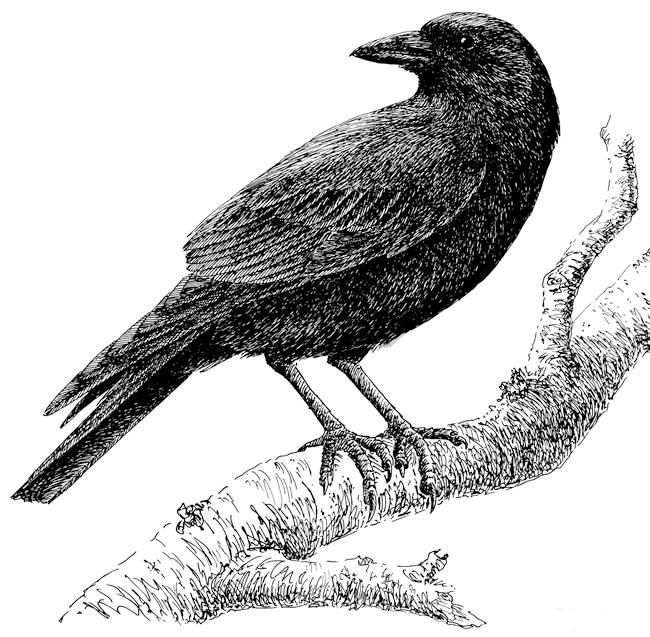
\includegraphics[width=\linewidth]{image}}\\[2\baselineskip]
      {\noindent\Huge\bfseries Дополнительные главы теории вероятностей}\\[\baselineskip]
      {\large\textrm{Конспекты лекций}}\\[3\baselineskip]
      {\Large\textsc{Лектор: Д.А. Шабанов}}\\[\baselineskip]
      {Конспект вел Данила Кутенин}\\[6\baselineskip]
      {\noindent НИУ ВШЭ, 2016-2017}\\[\baselineskip]
    }
  }
  \endgroup
}


\begin{document}
  \selectlanguage{russian}
  \pagestyle{empty}
  \titlepage
  \tableofcontents

  \setcounter{theorem}{0}
  \setcounter{definition}{0}
  \pagestyle{empty}
  \chapter{Допополнительные главы теории вероятностей}
  \pagestyle{fancy}
  \section{Лекция от 24.01.2017}

\epigraph{<<На прошлой лекции Дмитрий Александрович запнулся, на этой посмотрел записи. Ну всё, действительно сложный ТеорВер начался.>>}
{Один из слушателей}

\subsection{Случайные процессы}

\begin{definition}
  Пусть есть множество $T$ (неформально оно обозначает время). Набор случайных
  величин $(x_t, t \in T)$ будем называть \emph{случайным процессом.}
\end{definition}

\begin{remark}
  То, что написано в определении, на самом деле, называется \emph{случайной функцией},
  но для определенности оставим определение в таком же виде, потому что в основном
  будем использовать $T \subseteq \R$, что уже действительно является случайным
  процессом по определению во многих учебниках.
\end{remark}

\begin{definition}
  Классифицируем случайные процессы:
  \begin{itemize}
    \item если $T = \N, \Z, \Z_{+}$ --- случайный процесс с дискретным временем.
    \item если $T = [a, b], \R, \R_{+}$ --- случайный процесс с непрерывным
    временем.
    \item если $T \subseteq \R^d, d > 1$, тогда случайный процесс будет случайным
    полем.
  \end{itemize}
\end{definition}

Сейчас уделим больше внимания дискретным процессам. Будем считать, что у нас
задана тройка Колмогорова $(\Omega, \F, \Pr)$ и все $x_t: \Omega \to \R$.

\begin{definition}
  Для фиксированного $\omega_0 \in \Omega$ функция $\tilde{x}_t(t) = x_t(\omega_0), t \in T$
  является \emph{траекторией} (или \emph{реализацией}) случайного процесса.
\end{definition}

\begin{example}
  $x_t = f(t) \xi$, где $f(t)$ --- какая-то функция, $\xi$ --- случайная величина.
  Приведем пример траекторий для некоторых $\omega_0$.
  \begin{center}
    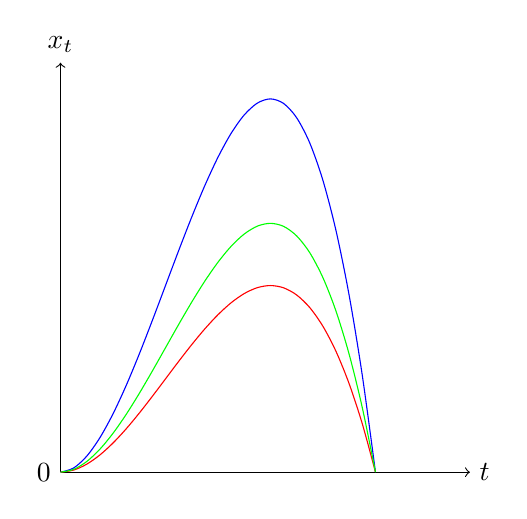
\begin{tikzpicture}
        \draw[->] (0,0) -- (5.2,0) node[right] {$t$};
        \draw[->] (0,0) -- (0,5.2) node[above] {$x_t$};
        \draw (0,0) node[left] {$0$};
        \draw[scale=1,domain=0:4,smooth,variable=\t,blue] plot ({\t},{2*\t*\t - \t*\t*\t/2)});
        \draw[scale=1,domain=0:4,smooth,variable=\x,red] plot ({\x},{\x*\x - \x*\x*\x/4)});
        \draw[scale=1,domain=0:4,smooth,variable=\x,green] plot ({\x},{4*\x*\x/3 - \x*\x*\x/3)});
    \end{tikzpicture}
  \end{center}
\end{example}

\subsection{Случайные блуждания}

\begin{definition}
  Пусть $\{\xi_n, \in \N\}$ --- независимые случайные величины. Определим
  $S_0 = 0$, а $S_n = \xi_1 + \ldots \xi_n, n \in \N$. Тогда $\{S_n, n \in \Z_{+}\}$
  называют \emph{случайным блужданием}.   
\end{definition}

\begin{center}
  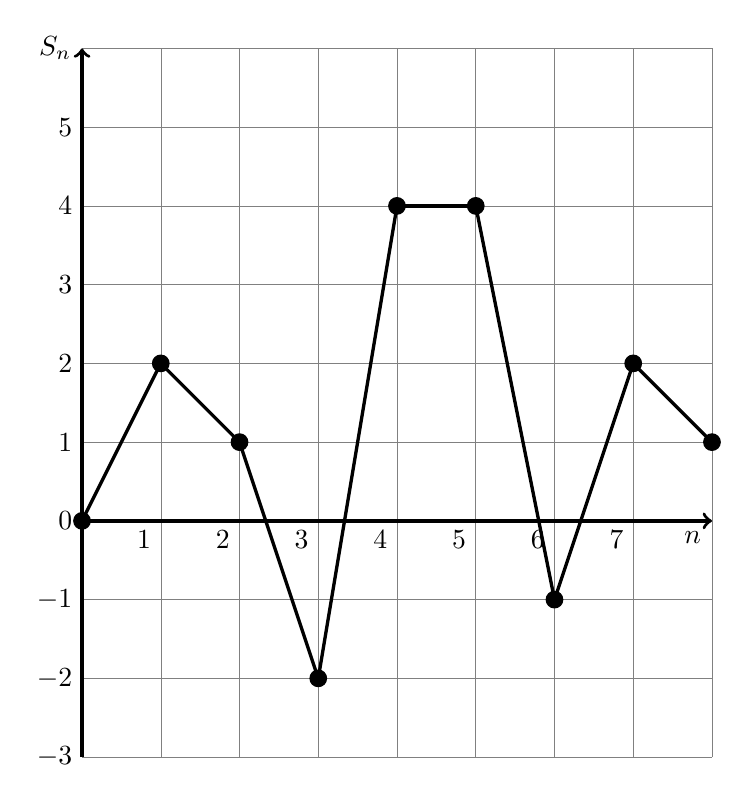
\begin{tikzpicture}
  
  \draw[step=1cm,gray,very thin] (2,-5) grid (10,4);
  \draw[very thick,->] (2,-2) -- (10,-2) node[anchor=north, below left] {$n$};
  \draw[very thick,->] (2,-5) -- (2, 4) node[anchor=east] {$S_n$};

  \node [left] at (2, -5) {$-3$};
  \node [left] at (2, -4) {$-2$};
  \node [left] at (2, -3) {$-1$};
  \node [left] at (2, -1) {$1$};
  \node [left] at (2, 0) {$2$};
  \node [left] at (2, 1) {$3$};
  \node [left] at (2, 2) {$4$};
  \node [left] at (2, 3) {$5$};

  \node [below left] at (3, -2) {$1$};
  \node [below left] at (4, -2) {$2$};
  \node [below left] at (5, -2) {$3$};
  \node [below left] at (6, -2) {$4$};
  \node [below left] at (7, -2) {$5$};
  \node [below left] at (8, -2) {$6$};
  \node [below left] at (9, -2) {$7$};

  
  \node [left] at (2, -2) {$0$};
  
  \draw (2, -2) node[draw,circle,fill=black,minimum size=6pt,inner sep=2pt] (C) {};
  \draw (3, 0) node[draw,circle,fill=black,minimum size=6pt,inner sep=2pt] (C) {};
  \draw (4, -1) node[draw,circle,fill=black,minimum size=6pt,inner sep=2pt] (C) {};
  \draw (5, -4) node[draw,circle,fill=black,minimum size=6pt,inner sep=2pt] (C) {};
  \draw (6, 2) node[draw,circle,fill=black,minimum size=6pt,inner sep=2pt] (C) {};
  \draw (7, 2) node[draw,circle,fill=black,minimum size=6pt,inner sep=2pt] (C) {};
  \draw (8, -3) node[draw,circle,fill=black,minimum size=6pt,inner sep=2pt] (C) {};
  \draw (9, 0) node[draw,circle,fill=black,minimum size=6pt,inner sep=2pt] (C) {};
  \draw (10, -1) node[draw,circle,fill=black,minimum size=6pt,inner sep=2pt] (C) {};

  \draw[very thick, -] (2, -2) -- (3, 0);
  \draw[very thick, -] (3, 0) -- (4, -1);
  \draw[very thick, -] (4, -1) -- (5, -4);
  \draw[very thick, -] (5, -4) -- (6, 2);
  \draw[very thick, -] (6, 2) -- (7, 2);
  \draw[very thick, -] (8, -3) -- (7, 2);
  \draw[very thick, -] (8, -3) -- (9, 0);
  \draw[very thick, -] (10, -1) -- (9, 0);
  \end{tikzpicture}
\end{center}


\begin{example}
  Физической моделью, соответствующую случайному блужданию, могут являться прыжки
  кузнечика.
\end{example}

\subsection{Процесс восстановления}

\begin{definition}

  Пусть $\{\xi_n, n \in \N\}$ --- одинаково распределенные
  неотрицательные случайные величины. Положим $S_0 = 0, S_n = \xi_1 + \ldots \xi_n,
  n \in \N$, а также для каждого $t \geq 0$ рассмотрим такие случайные величины:
  $x_t = \max\{n : S_n \leq t\}$ (если максимума не существует, положим $x_t = +\infty$).

  Процесс $(x_t, t \geq 0)$ называется \emph{процессом восстановления} для
  случайных величин $\{\xi_n, n \in \N\}$.
\end{definition}

График можно описать как-то так для какого-то $\omega_0$:


\begin{center}
  \begin{tikzpicture}
  
  \draw[line width=0.01mm,->] (0, 0) -- (12, 0) node[anchor=north, below left] {$t$};
  \draw[line width=0.01mm,->] (0, 0) -- (0, 7) node[anchor=east] {$x_t$};

  \draw (2.25, 0) node[draw,circle,fill=none,minimum size=4pt,inner sep=2pt] (C) {};
  \draw (5.46, 1) node[draw,circle,fill=none,minimum size=4pt,inner sep=2pt] (C) {};
  \draw (9.8, 2) node[draw,circle,fill=none,minimum size=4pt,inner sep=2pt] (C) {};
  \draw (11.7, 4) node[draw,circle,fill=none,minimum size=4pt,inner sep=2pt] (C) {};

  \draw[very thick, -] (0, 0) -- (2.25, 0);
  \draw[very thick, -] (2.25, 1) -- (5.46, 1);
  \draw[very thick, -] (5.46, 2) -- (9.8, 2);
  \draw[very thick, -] (11.7, 4) -- (9.8, 4);

  \draw[very thick, dashed, -] (0, 1) -- (2.25, 1);
  \draw[very thick, dashed, -] (0, 2) -- (5.46, 2);
  \draw[very thick, dashed, -] (0, 4) -- (9.8, 4);

  \node [left] at (0, 0) {$0$};
  \node [left] at (0, 1) {$1$};
  \node [left] at (0, 2) {$2$};
  \node [left] at (0, 3) {$3$};
  \node [left] at (0, 4) {$4$};

  \node [below] at (2.25, 0) {$S_1$};
  \node [below] at (5.46, 0) {$S_2$};
  \node [below] at (9.8, 0) {$S_3, S_4$};


  \end{tikzpicture}
\end{center}

Где возможны склеивания, как в $S_3, S_4$ --- это лишь означает, что $\xi_4 = 0$.

\begin{example}
  Физической моделью, соответствующую процессу восстановления, может служить
  процесс горения лампочки,
  где $\xi_n$ --- общее время горения $n$-ой лампочки, а $x_t$ тогда будет количеством
  поменянных лампочек до времени $t$.
\end{example}

Пара бы уже что-то доказать. Действительно, покажем, что мы не можем
часто убегать в бесконечность. На самом деле такие ситуации очень плохи в реальной
жизни. Происходит <<перенасыщение>> чего-то. В примере с лампочкой, мы можем менять
бесконечное число лампочек за время ноль. Такая ситуация очень плоха, поэтому,
чтобы успокоиться, докажем следующее утверждение:

\begin{theorem}
  Процесс восстановления конечен с вероятностью один, если $\Pr{\xi = 0} < 1$.
\end{theorem}

\begin{proof}
  Пусть $t > 0$ фиксировано. $\Pr{x_t = +\infty} = \Pr{\forall n : S_n \leq t}$.

  Заметим, что $S_n \leq S_{n + 1}$ из-за неотрицательности $\xi_{n + 1}$.

  Выпишем тривиальное равенство пределов:
  \[
    \lim\limits_{n \to +\infty} \Pr{S_n \leq t} = \lim\limits_{n \to +\infty} \Pr{\frac{S_n}{n} \leq \frac{t}{n}}
  \]

  Есть 2 случая:

  \begin{itemize}
    \item $\E{\xi_i}$ конечно и равно $A > 0$ (больше нуля, так как $\Pr{\xi_i = 0} < 1$).
    Тогда по закону больших чисел имеем,
    что $\frac{S_n}{n} \prto A$ (на самом деле мы немного лукавим, потому что
    в основном курсе эта теорема была доказана с использованием, что все моменты до четвёртого конечны,
    но ЗБЧ работает и при конечности средней величины).

    Тогда продолжим равенство пределов:

    \[
      = \lim\limits_{n \to +\infty} \Pr{\frac{S_n}{n} \leq \frac{t}{n}} \leq
      \lim\limits_{n \to +\infty} \Pr{\frac{S_n}{n} \leq \frac{A}{2}}
    \]

    Действительно, с какого-то момента $\frac{t}{n} < \frac{A}{2}$, так как
    $A > 0$. Далее, из закона больших чисел получаем:

    \[
      = \lim\limits_{n \to +\infty} \Pr{A \leq \frac{A}{2}} = 0.
    \]

    Последнее равенство идёт из-за неотрицательности $A$.

    Поэтому $\Pr{x_t = +\infty} = 0$ в этом случае.

    \item $\E{\xi_i} = +\infty$.

    Рассмотрим $\hat{\xi}_i = \min(\xi_i, 1) \leq \xi_i$. Откуда сразу получаем,
    что $\hat{S}_n = \hat{\xi}_1 + \ldots + \hat{\xi}_n \leq S_n$.

    Заметим, что $\E{\hat{S}_n}$ конечно, так как матожидание каждого из
    $\hat{\xi}_i$ конечно (так как $\hat{\xi}_i \leq 1$).

    А значит, что $\Pr{S_n \leq t} \leq \Pr{\hat{S}_n \leq t}$ (так как
    $S_n \geq \hat{S}_n$, а значит, что $\hat{S}_n$ принимает меньшие значения).

    Но мы уже всё доказали для конечного матожидания $\hat{\xi}_i$, поэтому получаем,
    что $\Pr{\hat{S}_n \leq t} \to 0$, откуда и $\Pr{S_n \leq t} \to 0$, что нам и требуется.
  \end{itemize}

\end{proof}

Приведём более мощный пример, обобщим эту модель.

\begin{example}
  Пусть $\{\xi_n, n \in \N\}$ --- независимые и одинаково распределенные
  случайные величины, $\{\eta_n, n \in \N\}$ --- независимые и одинаково
  распределенные случайные величины, притом независимы с $\{\xi_n, n \in \N\}$.

  Пусть $(x_t, t > 0)$ --- процесс восстановления, то есть
  $x_t = \max\{n : \xi_1 + \ldots + \xi_n \leq t\}$.

  Для $y_0, c > 0 \in \R$ введём

  \[
    Y_t = y_0 + ct - \sum\limits_{k = 1}^{x_t} \eta_k
  \]

  Эту модель называют моделью страхования Спарре-Андресена. Поясним, что значит
  каждая введенная переменная/величина.

  \begin{itemize}
    \item $y_0$ --- начальный капитал.
    \item $c$ --- скорость поступления страховых взносов. Для простоты считают,
    поступление линейно, что примерно одинаково <<бьются>> машины в любое время
    года.
    \item $\eta_k$ --- размер выплаты с номером $k$.
    \item $\xi_k$ --- время между $k - 1$-й и $k$-й выплатой.
    \item $x_t$ --- количество выплат к моменту времени $t$.
    \item $\sum\limits_{k = 1}^{x_t} \eta_k$ --- общий объём выплат по времени.
    \item И понятно, что тогда $Y_t$ --- текущий капитал.
  \end{itemize}

  В будущем, когда в нашем курсе мы затронем мартингалы, мы сможем понять и
  оценить, какова вероятность, что компания разорится.

  Ясно, что тогда график капитала от времени будет выглядеть примерно 
  таким образом:


\begin{center}
  \begin{tikzpicture}

  \draw[line width=0.01mm,->] (0, 0) -- (13, 0) node[anchor=north, below left] {$t$};
  \draw[line width=0.01mm,->] (0, 0) -- (0, 7) node[anchor=east] {$Y_t$};

  \draw[very thick, ->] (0, 2) -- (2, 5);
  \draw[very thick, dashed, -] (2, 5) -- (2, 2);
  \draw[very thick, ->] (2, 2) -- (3, 3.5);
  \draw[very thick, dashed, -] (3, 3.5) -- (3, 1);
  \draw[very thick, ->] (3, 1) -- (7, 7);
  \draw[very thick, dashed, -] (7, 7) -- (7, 5);
  \draw[very thick, ->] (7, 5) -- (7.8, 6.2);
  \draw[very thick, dashed, -] (7.8, 6.2) -- (7.8, 4.5);
  \draw[very thick, ->] (7.8, 4.5) -- (8.8, 6);

  \node [left] at (0, 2) {$y_0$};
  
  \node [below] at (2, 0) {$S_1$};
  \node [below] at (3, 0) {$S_2$};
  \node [below] at (7, 0) {$S_3$};
  \node [below] at (7.8, 0) {$S_4$};


  \end{tikzpicture}
\end{center}
\end{example}

\subsection{Простые случайные блуждания}

\begin{definition}
  Пусть $\{\xi_n, n \in \N\}$ независимые одинаково распределенные случайные
  величины такие, что для какого-то $p \in [0, 1]$
  \[
    \Pr{\xi_n = 1} = p, \Pr{\xi_n = -1} = 1 - p = q
  \]
  Положим $S_0 = 0, S_n = \xi_1 + \ldots \xi_n,
  n \in \N$. Тогда $\{S_n, n \in \Z_{+}\}$ называют \emph{простым случайным
  блужданием на прямой}.
\end{definition}

Смысл этого определения в том, что на каждом шаге мы выбираем с какими-то вероятностями, в какую сторону пойти.

Понятное дело, что этим можно не ограничиваться и, например, ходить в 4 разные
стороны на плоскости. Но давайте пока разберёмся с одномерным случаем.

\begin{definition}
  Если $p = q = \frac{1}{2}$, то говорят, что случайное блуждание симметрично.
\end{definition}

\begin{remark}
  Не лишним будет упомянуть, что в данном случае $\E{S_n} = (p - q)n$. 
  Действительно, если раскрыть по линейности, то совершенно ясно по 
  определению, что $\E{\xi_i} = p - q$.
\end{remark}

Перед нами возникают достаточно интересные вопросы:

\begin{itemize}
  \item[1.] Какова вероятность вернуться в ноль после ненулевого количества шагов?
  \item[2.] Какое среднее время мы проведем в нуле? 
  То есть сколько в среднем раз мы окажемся в нуле при достаточно больших $n$.
  \item[3.] Геометрия траекторий. То есть то, как выглядит график, какие существуют зависимости.
  Нашей кульминацией на этот вопрос будет закон повторного логарифма, который показывает,
  насколько далеко в среднем мы можем отходить от нуля.
\end{itemize}

Будем постепенно на все эти вопросы отвечать. Каждый из них --- отдельная
история, поэтому будем отвечать постепенно.

\subsection{Возвращение в ноль в простом случайном блуждании}

Легко понять, что нас интересует $\Pr{\exists \ n > 0 : S_n = 0}$.

Попробуем найти $\Pr{S_n = x}$. Во-первых, ясно, что $n$ и $x$ должны
быть одной четности, так как иначе мы не сможем из нуля прийти в $x$.
Также, нужно, чтобы $n \geq |x|$, иначе мы просто не дойдём до 
$x$, но скомпенсируем в будущем это тем, что $\binom{n}{k} = 0$ при $k > n$.

Пусть мы сделали $k$ шагов вправо и $n - k$ шагов влево. Под шагами 
подразумевается $+1$ и $-1$ соответственно. Тогда ясно, что
$k = \frac{n + x}{2}$, так как должно выполняться равенство $k - n + k = x$.

Поэтому получаем из-за того, что нам надо выбрать $k$ ходов, ответ для данной вероятности:

\[
  \Pr{S_n = x} = \binom{n}{k}p^kq^{n - k}I\{n + x \text{ чётно}\}
\]

Но этого мало. Мы не сможем как-то легко посчитать вероятность существования $n$, что $S_n = 0$.

Поэтому мы хотим понять, когда впервые достигнем нуля. Ясное дело, что нуля 
можно достигнуть только на четных ходах. Поэтому давайте посчитаем такую
вероятность:

\[
  \Pr{S_1 \neq 0, \ldots, S_{2n - 1} \neq 0, S_{2n} = 0}
\]

Заметим, что все $S_1, \ldots, S_{2n - 1}$ либо одновременно больше нуля,
либо все одновременно меньше нуля, так как из-за дискретной непрерывности,
если есть $S_i, S_j$ разных знаков, то найдётся между ними ноль, что 
противоречит тому, что мы ищем. 
Так как нам надо сделать $n$ ходов вправо и влево, эти случаи ничем не отличаются. Посчитаем вероятность, когда все $S_i > 0, i \in [2n - 1]$.

Посмотрим на траектории, которые у нас могут получиться:

\begin{center}
  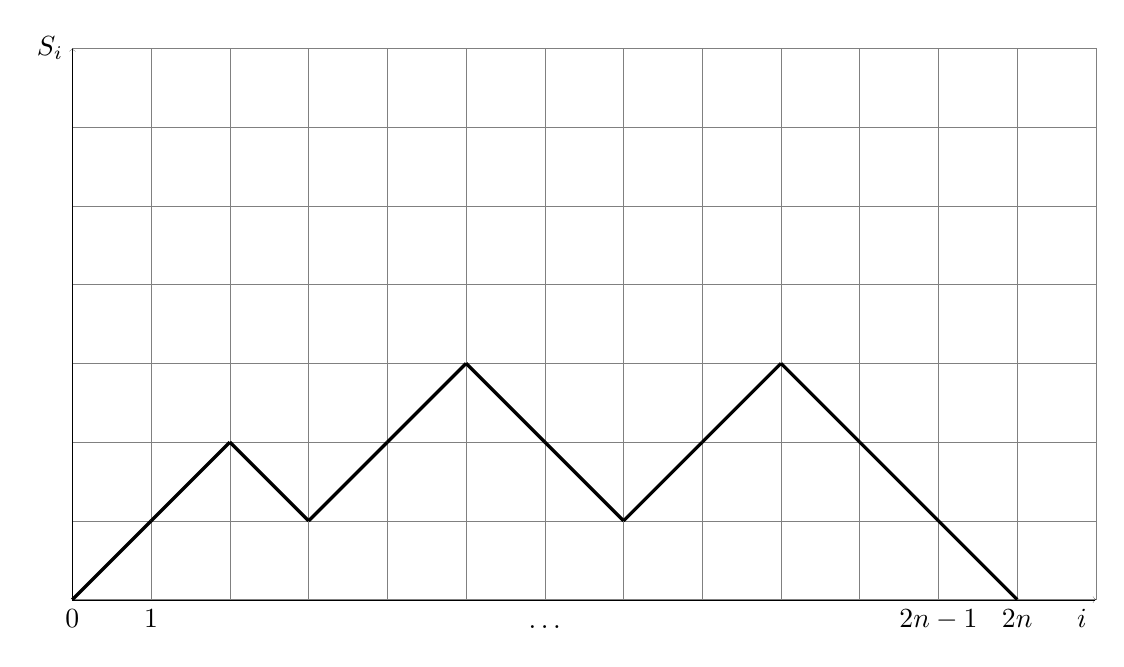
\begin{tikzpicture}

  \draw[step=1cm,gray,very thin] (0,0) grid (13,7);
  \draw[line width=0.01mm,->] (0, 0) -- (13, 0) node[anchor=north, below left] {$i$};
  \draw[line width=0.01mm,->] (0, 0) -- (0, 7) node[anchor=east] {$S_i$};


  \draw[very thick, -] (0, 0) -- (1, 1);
  \draw[very thick, -] (1, 1) -- (2, 2);
  \draw[very thick, -] (2, 2) -- (3, 1);
  \draw[very thick, -] (3, 1) -- (4, 2);
  \draw[very thick, -] (4, 2) -- (5, 3);
  \draw[very thick, -] (5, 3) -- (6, 2);
  \draw[very thick, -] (6, 2) -- (7, 1);
  \draw[very thick, -] (7, 1) -- (8, 2);
  \draw[very thick, -] (8, 2) -- (9, 3);
  \draw[very thick, -] (9, 3) -- (10, 2);
  \draw[very thick, -] (10, 2) -- (11, 1);
  \draw[very thick, -] (11, 1) -- (12, 0);

  \node [below] at (0, 0) {$0$};
  \node [below] at (1, 0) {$1$};
  \node [below] at (6, -0.2) {$\dots$};
  \node [below] at (11, 0) {${2n - 1}$};
  \node [below] at (12, 0) {${2n}$};
  \end{tikzpicture}
\end{center}

Теперь мы хотим посчитать все такие пути.

Обозначим через $\epsilon_i$ --- выбор $\pm1$ на $i$-ом шаге. Тогда путь подходит 
тогда и только тогда, когда $\sum\limits_{i = 1}^{2n} \epsilon_i = 0$ и
$\sum\limits_{i = 1}^{k} \epsilon_i > 0, k \in [2n - 1]$.

Обозначим количество таких путей через $\tilde{C}_n$.

А теперь вспомним, что числа Каталана задаются практически так же. Те, кто 
ходил на курс дискретной математики, помнят, что есть соответствие между 
числами Каталана и количеством путей, отвечающим свойствам: $\sum\limits_{i = 1}^{
2n} \epsilon_i = 0$ и
$\sum\limits_{i = 1}^{k} \epsilon_i \geq 0, k \in [2n - 1]$.

Обозначим количество таких путей через $C_n$.

\begin{lemma}
  $\tilde{C}_{n + 1} = C_{n}.$
\end{lemma}

\begin{proof}
  Рассмотрим любой путь, соответствующий $\tilde{C}_{n + 1}$. Заметим, что
  первые и последние шаги обязательно $+1$ и $-1$ соответственно. Поэтому, 
  при <<поднятии>> оси $Oi$ мы получим, что перед нами путь из $C_n$, 
  действительно, это так, так как префиксные суммы уменьшились на 1 и не стали 
  отрицательными, а сумма по-прежнему сохранилась нулевая.

  В другую сторону доказывается аналогично. См. иллюстрацию.

  \begin{center}
  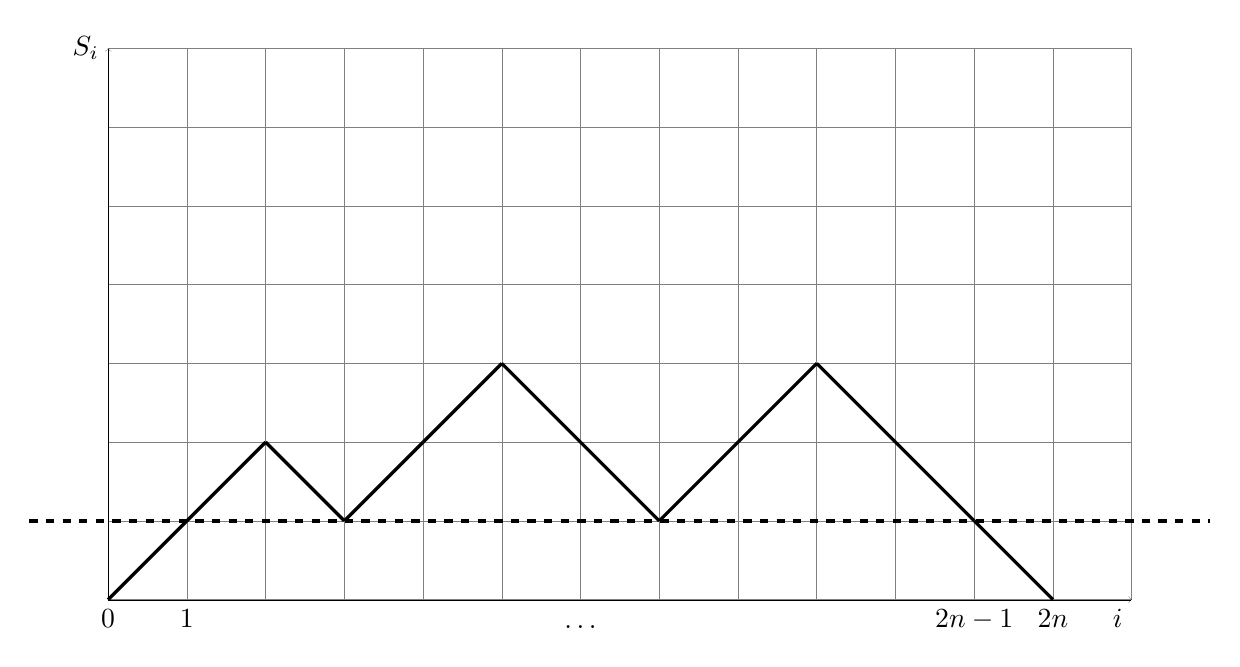
\begin{tikzpicture}

  \draw[step=1cm,gray,very thin] (0,0) grid (13,7);
  \draw[line width=0.01mm,->] (0, 0) -- (13, 0) node[anchor=north, below left] {$i$};
  \draw[line width=0.01mm,->] (0, 0) -- (0, 7) node[anchor=east] {$S_i$};


  \draw[very thick, -] (0, 0) -- (1, 1);
  \draw[very thick, -] (1, 1) -- (2, 2);
  \draw[very thick, -] (2, 2) -- (3, 1);
  \draw[very thick, -] (3, 1) -- (4, 2);
  \draw[very thick, -] (4, 2) -- (5, 3);
  \draw[very thick, -] (5, 3) -- (6, 2);
  \draw[very thick, -] (6, 2) -- (7, 1);
  \draw[very thick, -] (7, 1) -- (8, 2);
  \draw[very thick, -] (8, 2) -- (9, 3);
  \draw[very thick, -] (9, 3) -- (10, 2);
  \draw[very thick, -] (10, 2) -- (11, 1);
  \draw[very thick, -] (11, 1) -- (12, 0);
  \draw[very thick, dashed, -] (-1, 1) -- (14, 1);


  \node [below] at (0, 0) {$0$};
  \node [below] at (1, 0) {$1$};
  \node [below] at (6, -0.2) {$\dots$};
  \node [below] at (11, 0) {${2n - 1}$};
  \node [below] at (12, 0) {${2n}$};
  \end{tikzpicture}
\end{center}
\end{proof}

Получается, что

\[
  \Pr{S_1 > 0, \ldots, S_{2n - 1} > 0, S_{2n} = 0} = C_{n - 1}(pq)^n
\]

И соответственно:

\[
  \Pr{S_1 \neq 0, \ldots, S_{2n - 1} \neq 0, S_{2n} = 0} = 2C_{n - 1}(pq)^n
\]

Внимательный читатель заметит, что чтобы посчитать самую исходную 
вероятность, надо просто сложить все такие выше. О том, как такие вещи 
складывать (в частности о характеристических функциях), мы поговорим в
следующей лекции.


  \section{Лекция от 31.01.2017}

\subsection{Числа Каталана. Реккурентное соотношение. Производящая функция}
\begin{lemma}
  Обозначим $C_0 = 1$, тогда имеет место следующее равенство:

  \[
    C_n = \sum\limits_{k = 0}^{n - 1} C_k C_{n - 1 - k}
  \]
\end{lemma}

\begin{proof}
  Будем опять рассуждать в терминах положительной траектории (см. рис с предыдущей
  лекции).

  Пусть $2k > 0$ первый момент, когда наша траектория придёт в ноль. Действительно,
  такой момент найдётся, потому что в момент времени $2n$ мы придём в ноль.

  Тогда от $0$ до $2k$ положительная траектория, от $2k$ до $2n$ неотрицательная,
  поэтому всего таких путей $\tilde{C}_{k}C_{n - k}$. Чтобы получить все траектории,
  надо сложить все такие вещи по всем $k = 1, \ldots, n$, поэтому мы получим,
  что имеет место равенство по последней лемме из предыдущей лекции и тем, что $C_0 = 1$:
  \[
    C_n = \sum\limits_{k = 1}^n \tilde{C}_{k}C_{n - k} =
    \sum\limits_{k = 1}^n C_{k - 1}C_{n - k} = \text{<<замена $j = k - 1$>>} =
    \sum\limits_{j = 0}^{n - 1} C_j C_{n - 1 - j}
  \]
\end{proof}

\begin{definition}
  Для последовательности $\{a_n\}_{n = 0}^{+\infty}$ производящей функцией называется $f(x) = \sum\limits_{n = 0}^{+\infty} a_n x^n$.
\end{definition}

Ряд может расходится на некоторых $x$ и тогда мы просто
рассматриваем ряд формально, на них можно ввести операции сложения
и прочие операции.

Заметим, что $C_n \leq 2^{2n}$, 
потому что всего путей не больше $2^{2n}$, на самом деле их меньше
аж примерно в $n^{3/2}$ раза, но это нам нужно для того, чтобы 
производящая функция чисел Каталана была такова, что при 
$|x| < \frac{1}{4}$ ряд сходился. Как мы потом увидим, он будет 
сходится и при $|x| = \frac{1}{4}$.

Сейчас мы будем рассматривать только $f(x) = \sum\limits_{n = 0}^{+\infty}
C_n x^n$ при $|x| < \frac{1}{4}$.

\begin{theorem}
  $f(x) = \dfrac{1 - \sqrt{1 - 4x}}{2x}$.
\end{theorem}

\begin{proof}
  \[
    f^2(x) = \left(\sum\limits_{n = 0}^{+\infty} C_n x^n\right)^2 = 
    \sum\limits_{n = 0}^{+\infty}\left(\sum\limits_{k = 0}^{n} C_k C_{n - k}\right) x^n.
  \]

  Внимательный читатель заметит, что мы в скобках в точности получили реккурентное
  соотношение для чисел Каталана для $C_{n + 1}$. Поэтому это равно:

  \[
    \sum\limits_{n = 0}^{+\infty}\left(\sum\limits_{k = 0}^{n} C_k C_{n - k}\right) x^n
    = \sum\limits_{n = 0}^{+\infty} C_{n + 1}x^n = \frac{f(x) - 1}{x}.
  \]

  Где последнее равенство возникает из-за того, что $C_0 = 1$.

  Откуда мы получаем квадратное уравнение относительно $f(x)$.

  \[
    xf^2(x) - f(x) + 1 = 0.
  \]

  Решая уравнение, получим, что

  \[
    f(x) = \frac{1 \pm \sqrt{1 - 4x}}{2x}
  \]

  Но мы знаем, что $f(0) = 1$, поэтому с плюсом не подходит, так как предел
  будет не тот. Откуда единственный подходящий вариант будет

  \[
    f(x) = \frac{1 - \sqrt{1 - 4x}}{2x}
  \]
\end{proof}

Заметим, что и при $\frac{1}{4}$ мы получим конечное число, поэтому по непрерывности
можно сказать, что и в $x = \frac{1}{4}$ ряд сходится.

\subsection{Вероятность возвращения}

\begin{theorem}
  Случайное блуждание возвратно с вероятностью $1 - |p - q|$.
\end{theorem}

\begin{proof}
  Заметим, что подставить $pq$ в производящую функцию можно, так как 
  $pq \leqslant \frac{1}{4}$.

  \begin{multline}
    \Pr{\exists n : S_n = 0} = \sum\limits_{n = 1}^{+\infty} \Pr{S_1 \neq 0, 
    \ldots, S_{2n - 1} \neq 0, S_{2n} = 0} =\\= \sum\limits_{n = 1}^{+\infty}
    2C_{n - 1}(pq)^n = 2pq\sum\limits_{n = 0}^{+\infty} C_n (pq)^n =
    2pq\frac{1}{2pq}(1 - \sqrt{1 - 4pq}) = \text{<<так как $1 = (p + q)^2$>>} =\\=
    1 - \sqrt{(p - q)^2} = 1 - |p - q|
  \end{multline}
\end{proof}

\begin{remark}
  Если $p = q = \frac{1}{2}$, то случайное блуждание возвратно с вероятностью один.
\end{remark}

\subsection{Многомерный случай}

Абстрактно поговорим о многомерном случае. То есть мы находимся в $\Z^d, d > 1$.

На плоскости мы можем идти в 4 разные стороны с равными вероятностями.
Как ни странно, вероятность возвращения в ноль в данном случае будет тоже равна один.

\begin{center}
  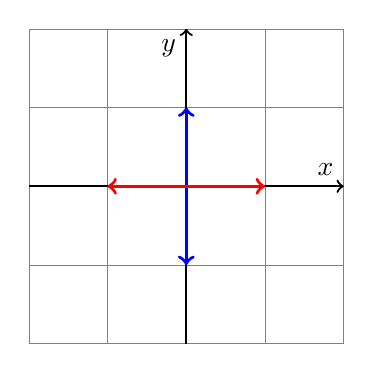
\begin{tikzpicture}
  
  \draw[step=1cm,gray,very thin] (-2,-2) grid (2,2);
  \draw[thick,->] (0,-2) -- (0,2) node[anchor=north, below left] {$y$};
  \draw[thick,->] (-2,0) -- (2, 0) node[anchor=east, above left] {$x$};

  \draw[very thick,->,blue] (0,0) -- (0, 1) node[anchor=east, above left] {};
  \draw[very thick,->,blue] (0,0) -- (0, -1) node[anchor=west, above left] {};
  \draw[very thick,->,red] (0,0) -- (1, 0) node[anchor=north, above left] {};
  \draw[very thick,->,red] (0,0) -- (-1, 0) node[anchor=south, above left] {};

  \end{tikzpicture}
\end{center}


В трёхмерном случае не всё так однозначно. У нас есть шесть направлений. И в данном
случае вероятность возвращения будет строго меньше единицы. С этим разобраться
мы предложим читателю в будущих задачах.

\begin{center}
  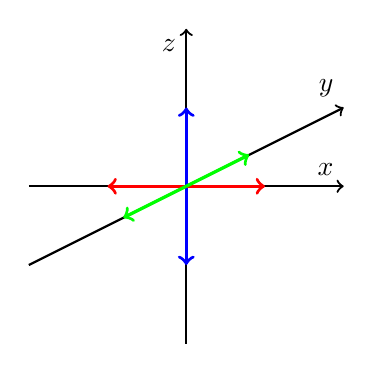
\begin{tikzpicture}
  
  \draw[thick,->] (0,-2) -- (0,2) node[anchor=north, below left] {$z$};
  \draw[thick,->] (-2,0) -- (2, 0) node[anchor=east, above left] {$x$};
  \draw[thick,->] (-2,-1) -- (2, 1) node[anchor=east, above left] {$y$};

  \draw[very thick,->,blue] (0,0) -- (0, 1) node[anchor=east, above left] {};
  \draw[very thick,->,blue] (0,0) -- (0, -1) node[anchor=west, above left] {};
  \draw[very thick,->,red] (0,0) -- (1, 0) node[anchor=north, above left] {};
  \draw[very thick,->,red] (0,0) -- (-1, 0) node[anchor=south, above left] {};
  \draw[very thick,->,green] (0, 0) -- (0.8,0.4) node[anchor=south, above left] {};
  \draw[very thick,->,green] (0, 0) -- (-0.8,-0.4) node[anchor=south, above left] {};


  \end{tikzpicture}
\end{center}

На самом деле всё это зависит от $\Pr{S_{2n} = 0}$. При $d = 1$ и $p = q = \frac{1}{2}$
получим, что $\Pr{S_{2n} = 0} = \binom{2n}{n}4^{-n} \approx \Theta\left(\frac{1}{\sqrt{n}}\right)$, ряд расходится.

При $d = 2$ будет $\Theta\left(\frac{1}{n}\right)$, что тоже расходится, с каждой
новой размерностью добавляется этот самый $\sqrt{n}$ в знаменателе, поэтому
с $d = 3$ ряд будет сходящимся. Это была подсказка на будущие задачи, ничего
тут мы пока не доказывали.

\subsection{Числа Каталана через биномиальные коэффициенты}
Вспомним некоторые факты про ряд Тейлора, а именно, что

\[
  (1 + x)^{\alpha} = \sum\limits_{n = 0}^{+\infty} \binom{\alpha}{n}x^n,
\]

где $\binom{\alpha}{n} = \frac{\alpha(\alpha - 1)\ldots (\alpha - n + 1)}{n!}$.

Поэтому давайте преобразуем ряд для $f(x) = \sum\limits_{n = 0}^{+\infty} C_n x^n$.

\[
  \sqrt{1 - 4x} = \sum\limits_{n = 0}^{+\infty} \binom{1/2}{n}x^n = 
  1 + \sum\limits_{n = 1}^{+\infty} \frac{\frac{1}{2}\left(\frac{1}{2} - 1\right)
  \ldots\left(\frac{1}{2} - n + 1\right)}{n!}(-4x)^n = 
\]

Вынесем $1/2$ из каждой дроби, везде поменяем знак, получим, что это домножится
на $(-1)^{n - 1}$, что совместно с $(-4x)^n$ даст знак минус, в скобках
останется $(2n - 3)!!$:

\[
  = 1 - \sum\limits_{n = 1}^{+\infty} \frac{4^n x^n (2n - 3)!!}{2^n n!} =
  1 - \sum\limits_{n = 1}^{+\infty} \frac{2^n x^n (2n - 3)!!}{n!} = 
\]

Домножим на $n!$ и разделим на него, а также домножим на $2n - 1$ и опять же
разделим. Воспользуемся тем, что $(2n)! = (2n - 1)!! n! \cdot 2^n$:

\[
  = 1 - \sum\limits_{n = 1}^{+\infty} \frac{(2n)!x^n}{n!n!}\frac{1}{2n - 1} =
  1 - \sum\limits_{n = 1}^{+\infty} \binom{2n}{n} \frac{x^n}{2n - 1}
\]

Откуда:

\[
  f(x) = \frac{1}{2x}(1 - \sqrt{1 - 4x}) = \frac{1}{2}\sum\limits_{n = 1}^{+\infty}
  \binom{2n}{n} \frac{1}{2n - 1}x^{n - 1} = 
  \frac{1}{2}\sum\limits_{n = 0}^{+\infty} \binom{2n + 2}{n + 1} \frac{1}{2n + 1}x^{n} =
  \sum\limits_{n = 0}^{+\infty} \binom{2n}{n} \frac{1}{n + 1}x^{n}
\]

В последнем равенстве можно убедиться непосредственно.

Откуда получаем $C_k = \frac{1}{k + 1}\binom{2k}{k}$.

\begin{remark}
  $\Pr{S_1 \neq 0, \ldots, S_{2n - 1} \neq 0, S_{2n} = 0} = 2C_{n - 1}(pq)^n =
  \binom{2n}{n}(pq)^n\frac{1}{2n - 1}$ --- распределение первого момента в нуле.
\end{remark}

\subsection{Математическое ожидание первого момента возвращения в ноль}

\begin{definition}
  $X = \min(2n : S_{2n} = 0)$.
\end{definition}

\begin{theorem}
  $\E{X} = +\infty$.
\end{theorem}

\begin{proof}
  Если $p \neq q$, тогда $\Pr{x = +\infty} > 0$, поэтому матожидание уже
  точно бесконечность.

  Если $p = q = \frac{1}{2}$, тогда $\E{X} = \sum\limits_{n = 1}^{+\infty}
  \Pr{X = 2n}\cdot (2n) = \sum\limits_{n = 1}^{+\infty} \binom{2n}{n} 
  \frac{2n}{2n - 1}\frac{1}{4^n} = \Theta\left(\frac{1}{\sqrt{n}}\right)$, что расходится
\end{proof}

Получается, что да, в ноль мы вернемся, но очень не скоро и бесконечно долго будем
ходить вне. Вот такой вот парадокс. Перейдём к следующему пункту.

\subsection{Среднее время в нуле}

Оказывается, что в нуле мы будем находится не так мало. За $n$ шагов примерно
$\sqrt{n}$ раз мы будем в нуле. Это по большей мере связано с тем, что нули
расположены рядом, то есть есть большая вероятность, что если мы пришли в ноль,
то через малое количество шагов окажемся опять там.

\begin{definition}
  Будем рассматривать симметричное простое случайное блуждание. Тогда 
  $L_n = \left|k : k \in \overline{0, \ldots, n}, S_k = 0\right|$.
\end{definition}

Хотим понять, какая асимптотика у $\E{L_n}$.

\begin{lemma}
  $\E{L_n} = \E{|S_{n + 1}|}$
\end{lemma}

\begin{proof}
  Распишем $|S_{n+1}|$:
  \[
  |S_{n + 1}| =
  \begin{cases}
    1, \text{если $|S_n| = 0$}\\
    S_n + \xi_{n + 1}, \text{если $S_n > 0$}\\
    -S_n - \xi_{n + 1}, \text{если $S_n < 0$}
  \end{cases}
  \]
  Действительно, при положительном $S_n$ мы не поменяем знак, поэтому
  надо лишь добавить то, что мы выбирали на следующем ходу, при отрицательном
  $S_n$ аналогично, а если $S_n = 0$, то в любом случае модуль равен единице.

  Запишем $|S_{n + 1}|$ через индикаторы:

  \[
    |S_{n + 1}| = \I\{|S_n| = 0\} + (S_n + \xi_{n + 1})\I\{S_n > 0\} -(S_n + \xi_{n + 1})\I\{S_n < 0\}
  \]

  Заметим, что $S_n \I\{S_n > 0\} - S_n \I\{S_n < 0\} = |S_n|$ (в этом легко
  убедиться, проверив несколько случаев). Поэтому, введя функцию знака, можно
  утверждать, что:
  \[
   |S_{n + 1}| = \I\{|S_n| = 0\} + |S_n| + \xi_{n + 1}\mathrm{sgn}(S_n)
  \]

  Будем раскрывать рекурсивно, откуда получим:

  \[
    |S_{n + 1}| = \sum\limits_{k = 0}^{n} \I\{|S_k| = 0\} + |S_0| +
    \sum\limits_{k = 0}^{n} \xi_{k + 1}\mathrm{sgn}(S_{k})
  \]

  Заметим, что $L_n = \sum\limits_{k = 0}^{n} \I\{|S_k| = 0\}$, поэтому давайте
  запишем под знаком матожидания с использованием, что $\E{|S_0|} = 0$.

  \[
    \E{|S_{n + 1}|} = \E{L_n} + \sum\limits_{k = 0}^{n} \E{\xi_{k + 1}\mathrm{sgn}(S_{k})}
  \]
  Но величины $\xi_{k + 1}$ и $\mathrm{sgn}(S_{k})$ независимы, так как нет
  пересечений по ходам, поэтому это распадается в произведение матожиданий.

  Ну и финальный аккорд состоит в том, что $\E{\xi_{k + 1}} = 0$, поэтому
  мы доказали равенство.
\end{proof}

Про асимптотику поговорим в следующей лекции.

  \section{Лекция от 07.02.2017}

\subsection{Среднее время в нуле}

Вспомним, что по ЦПТ и тем фактом, что среднее $\xi_i$ равно нулю и дисперсия равна 
единице мы имеем следующее:

\[
  \frac{S_n}{\sqrt{n}} \dto \mathcal{N}(0, 1)
\]

По теореме о наследовании сходимости можно заключить, что

\[
  \frac{|S_n|}{\sqrt{n}} \dto |\mathcal{N}(0, 1)|
\]

А теперь мы хотим осознать, а как ведет себя среднее левой части. Заметим, что
просто матожидание мы не можем взять, так как функция $f(x) = x$ не ограничена
и эквивалентным определением сходимости по распределению напрямую воспользоваться
нельзя. Поэтому нужны более сильные знания о поведений случайных величин.

\begin{definition}
  Последовательность $\{\xi_n, n \in \N\}$ называется равномерно интегрируемой,
  если

  \[
    \lim\limits_{c \to +\infty} \sup\limits_{n \in \N} \E{|\xi_n|\I\{|\xi_n| \geq c\}} = 0
  \]
\end{definition}

Поясним определение.

Если у случайной величины есть плотность, то фактически мы говорим, что

\[
  \sup\limits_{n \in \N} \int\limits_{|x| \geq c} |x| p_{\xi_n}(x) dx \to 0
\]

То есть модуль среднего на бесконечности в обе стороны близок к нулю.

\begin{theorem}
  Пусть $\xi_n \dto \xi, \xi_n \geq 0$ --- все величины с конечным матожиданием,
  тогда $\E{\xi_n} \to \E{\xi}$ тогда
  и только тогда, когда последовательность $\{\xi_n, n \in \N\}$ равномерно 
  интегрируема.
\end{theorem}

\begin{proof}
  Докажем в одну сторону, в другую оставим в качестве домашней задачи.

  Пусть последовательность равномерно интегрируема. Тогда для $c > 0$ рассмотрим
  функцию $f_c(x)$:

  \begin{center}
    \begin{tikzpicture}
    
    \draw[very thick,->] (-3,0) -- (10,0) node[anchor=north, below left] {$x$};
    \draw[very thick,->] (0,0) -- (0, 7) node[anchor=east] {$f_c(x)$};

    \node [below] at (0, 0) {$0$};
    \node [below] at (5, 0) {$c$};
    \node [below] at (6, 0) {$c + 1$};
    \node [above left] at (4, 4) {$x = f_c(x)$};


    \draw[very thick, -, blue] (-3, 0) -- (0, 0);
    \draw[very thick, -, blue] (-3, 0) -- (0, 0);
    \draw[very thick, -, blue] (0, 0) -- (5, 5);
    \draw[very thick, -, blue] (5, 5) -- (6, 0);
    \draw[very thick, -, blue] (6, 0) -- (9, 0);
    \draw[very thick, -, dashed] (5, 5) -- (5, 0);

    \end{tikzpicture}
  \end{center}

  То есть до $0$ эта функция тождественно ноль, потом ведет себя так же, как
  и аргумент до $c$, потом резко убывает и снова становится нулем. Мы вводим
  такую функцию, чтобы приблизить $f(x) = x$, но ограниченным образом.

  Заметим, что $f_c(x)$ непрерывна и ограничена. Оценим $|\E{\xi_n} - \E{\xi}|$.
  Добавим и вычтем каждое из двух выражений под модулем $\E{f_c(\xi_n)}, \E{f_c(\xi)}$
  и воспользуемся неравенством треугольника:

  \[
    |\E{\xi_n} - \E{\xi}| \leq |\E{\xi_n} - \E{f_c(\xi_n)}| + 
    |\E{\xi} - \E{f_c(\xi)}| + |\E{f_c(\xi_n)} - \E{f_c(\xi)}|
  \]

  Зафиксируем произвольное $\epsilon > 0$. Первое слагаемое не больше 
  $\E{\xi_n \I\{\xi_n \geq c\}}$, так как при $\xi_n \leq c$, величины просто
  совпадают, от $c$ до $c + 1$ будет какой-то остаток, не больший, чем $\E{\xi_n 
  \I\{c \leq \xi_n \leq c + 1\}}$, а дальше уже просто $\E{f_c(\xi_n)}$ не даёт
  никакого вклада. Откуда $\E{\xi_n \I\{\xi_n \geq c\}} \leq \frac{\epsilon}{2}$
  при всех $c > c_0(\epsilon)$. Эта оценка работает по условию теоремы при всех $n$.

  Второе слагаемое для всех $c > c_1(\epsilon)$ тоже не больше, чем $\frac{\epsilon}{2}$,
  так как мы приближаем $f_c(x)$ положительную функцию (и при $c \to +\infty$ $f_c(x) \to x$)
  и матожидание конечно, то с какого-то момента разность станет очень маленькой.

  Третье слагаемое стремится к нулю с ростом $n$ из-за эквивалентного определения
  сходимости по распределению.

  Поэтому получаем, что

  \[
    \forall \epsilon > 0 \varlimsup\limits_{n \to +\infty} |\E{\xi_n} - \E{\xi}| \leq \epsilon
  \]

  Откуда есть предел и равен он нулю, что и требовалось доказать.
\end{proof}


Но теперь, чтобы наконец-то понять асимптотику среднего в нуле, давайте
поймём, какие условия <<полегче>> нужно наложить, чтобы последовательность
была равномерно интегрируемой. Это можно сделать из следующей леммы:

\begin{lemma}
  Пусть $\{\xi_n, n \in \N\}$ --- последовательность случайных величин. Если
  для всех $n \in \N$ выполнено, что $\E{\xi_n^2} \leq C < +\infty$, тогда
  последовательность равномерно интегрируема.
\end{lemma}

\begin{proof}
  Для любого $\epsilon > 0$ выберем $t_0$ такое, что $t_0 > \frac{C}{\epsilon}$.
  Тогда для любого $t > t_0$ и любого $n \in \N$

  \[
    \E{|\xi_n|\I\{|\xi_n| \geq t\}} \leq \E{\frac{\xi_n^2}{t}\I\{|\xi_n| \geq t\}}
    \leq \frac{C}{t} \leq \frac{C}{t_0} < \epsilon
  \]

  Значит предел есть и равен нулю.
\end{proof}

Теперь сформулируем основную теорему:

\begin{theorem}
  \[
    \E{L_n} \sim \sqrt{\frac{2n}{\pi}}
  \]
\end{theorem}

\begin{proof}
  По последней лемме из прошлой лекции имеем $\E{L_n} = \E{|S_{n + 1}|}$.

  А также мы выяснили, что

  \[
    \frac{|S_n|}{\sqrt{n}} \dto |\mathcal{N}(0, 1)|
  \]

  Посмотрим на второй момент левой части и вспомним, что среднее у $S_n$ равно
  нулю:

  \[
    \E{\frac{S_n^2}{n}} = \frac{\D{S_n}}{n} = 1
  \]

  Последнее равенство следует из того, что дисперсия независимых величин равна
  сумме дисперсий.

  Получаем, что второй момент всегда ограничен единицей, значит по теореме 5
  мы получаем, что

  \[
    \E{\frac{|S_n|}{\sqrt{n}}} \to \E{|\mathcal{N}(0, 1)|} = \sqrt{\frac{2}{\pi}}
  \]

  Где последнее равенство легко проверяется интегрированием (см одно из ДЗ обычного
  курса).

  Получаем, что $\E{L_n} \sim \sqrt{\dfrac{2n}{\pi}}$
\end{proof}

\subsection{Геометрия траекторий. Закон повторного логарифма}

Начнём сразу с теоремы, потом будем пояснять её смысл и постепенно доказывать.

\begin{theorem}[Закон повторного логарифма]
  Пусть $\{S_n, n \in \Z_+\}$ --- простое симметричное случайное блуждание.

  Тогда 

  \[
    \Pr{\varlimsup\limits_{n \to +\infty} \frac{S_n}{\sqrt{2n\ln\ln n}} = 1} = 1
  \]
\end{theorem}

Выведем маленькое следствие из этого:

\begin{remark}
  Докажем, что из ЗПЛ следует следующий факт:

  \[
    \Pr{\varliminf\limits_{n \to +\infty} \frac{S_n}{\sqrt{2n\ln\ln n}} = -1} = 1
  \]

  Ну это легко понять, если заменить $S_n = -X_n$ и надо лишь осознать, что 
  $\{X_n, n \in \Z_+\}$
  тоже случайное блуждание, но это совершенно ясно из определения.
\end{remark}

Давайте будем пояснять смысл.

Закон повторного логарифма занимает промежуточное положение между законом 
больших чисел и центральной предельной теоремой. Мы знаем, что

\[
  \frac{S_n}{n} \prto 0, \frac{S_n}{\sqrt{n}} \dto \mathcal{N}(0, 1)
\]

Центральная предельная теорема утверждает, что суммы $S_{n}$ с делителем
$\sqrt{n}$ сходятся к стандартному нормальному распределению, и эта
последовательность сумм не сходится к какой-либо конкретной величине ни по
вероятности, ни почти наверное, а бесконечно блуждает.

Таким образом величина $S_{n}/{\sqrt{2n\ln \ln n}}$ будет
к любой точке отрезка $[-1, 1]$ бесконечное число раз приближаться
сколь угодно близко почти наверное.

Так же ЗПЛ означает, что с вероятностью один график блуждания лежит между 
$(1 + \epsilon){\sqrt{2n\ln \ln n}}$ и $-(1 + \epsilon){\sqrt{2n\ln \ln n}}$
для любого $\epsilon > 0$ и бесконечное число раз выходит за пределы
$(1 - \epsilon){\sqrt{2n\ln \ln n}}$ и $-(1 - \epsilon){\sqrt{2n\ln \ln n}}$.

Вспомним лемму Бореля-Кантеля, а сам ЗПЛ докажем на следующей лекции.

\begin{definition}
  Пусть $\{A_n, n \in \N\}$ -- события. Тогда событием $\{A_n \text{ беск. число}\}$
  (или $\{A_n \text{ б. ч.}\}$)
  называют $\bigcap\limits_{n = 1}^{+\infty}\left(\bigcup\limits_{m \geq n} A_m\right)$. Событие
  состоит в том, что произошло бесконечное число событий.
\end{definition}

\begin{theorem}[Лемма Бореля-Кантелли]
  Пусть $\{A_n, n \in \N\}$. 

  1) Если $\sum\limits_{n = 1}^{+\infty} \Pr{A_n}$ сходится,
  тогда $\Pr{\{A_n \text{ б. ч.}\}} = 0$.

  2) Если $\sum\limits_{n = 1}^{+\infty} \Pr{A_n}$ расходится и $A_n$ независимые
  величины,
  тогда $\Pr{\{A_n \text{ б. ч.}\}} = 1$.
\end{theorem}

\begin{proof}
  1)

  \[
    \Pr{\{A_n \text{ б. ч.}\}} = \Pr{\bigcap\limits_{n = 1}^{+\infty}\left(\bigcup\limits_{m \geq n} A_m\right)} =
    \lim\limits_{n \to +\infty} \Pr{\bigcup\limits_{m \geq n} A_m} \leq
    \lim\limits_{n \to +\infty} \sum\limits_{m \geq n} \Pr{A_m} = 0
  \]

  Последнее равенство верно, так как остаток сходящего ряда стремится к нулю.

  2) Тут уже напрямую не получится, надо провести более тонкий анализ:

  \[
     \Pr{\{A_n \text{ б. ч.}\}} =  \lim\limits_{n \to +\infty} 
     \Pr{\bigcup\limits_{m \geq n} A_m} = 1 - \lim\limits_{n \to +\infty}
     \Pr{\bigcap\limits_{m \geq n} \overline{A_m}} = 
  \]

  Хочется воспользоваться независимостью, но в данном случае надо применять один
  трюк, чтобы это стало возможным. Поставим повторный предел:

  \[
    =  1 - \lim\limits_{n \to +\infty}\lim\limits_{N \to +\infty} \Pr{\bigcap\limits_{m = n}^{N} \overline{A_m}} = 
  \]

  Вот теперь уже можно пользоваться независимостью событий (а значит и их
  дополнений).

  \[
    1 - \lim\limits_{n \to +\infty}\lim\limits_{N \to +\infty} \prod_{m = n}^{N}(1 -
    \Pr{A_m}) 
  \]

  Применим неравенство, что $1 - x \leqslant e^{-x}$ и поэтому можно написать, что

  \[
    1 - \lim\limits_{n \to +\infty}\lim\limits_{N \to +\infty} \prod_{m = n}^{N}(1 -
    \Pr{A_m}) \geq 1 - \lim\limits_{n \to +\infty}\lim\limits_{N \to +\infty}
    e^{-\sum\limits_{m = n}^{N} \Pr{A_m}}
  \]

  Но остаток расходящегося ряда стремится к $+\infty$, поэтому имеем равенство

  \[
    = 1 - \lim\limits_{n \to +\infty}e^{-\infty} = 1
  \]
\end{proof}

  \section{Лекция от 14.02.2017}

\subsection{Закон повторного логарифма}

В этой лекции докажем этот закон и поймём, что обычной техникой оценивания
через ЦПТ и некоторые другие теоремы вообще не работают.

Вспомним, что мы хотим глобально. Введем 2 события для произвольного $\epsilon > 0$:

\[
  A_n = \{S_n \geq (1 + \epsilon)\sqrt{2n\ln\ln n}\},
  B_n = \{S_n \geq (1 - \epsilon)\sqrt{2n\ln\ln n}\}
\]

Чтобы доказать утверждение теоремы, надо показать, что

\[
  \Pr{\{\text{$A_n$ б.ч.}\}} = 0;
  \Pr{\{\text{$B_n$ б.ч.}\}} = 1
\]

\subsection{Следствие из ЦПТ и теоремы Берри-Эссеена}

Если вспомнить ЦПТ и теорему Берри-Эссеена, тогда (учитывая, что третий момент конечен и
$\E{\xi_1} = 0, \D{\xi_1} = 1$) получаем, что

\[
  \sup\limits_{x \in \R} 
  \left|\Pr{\frac{S_n - n\E{\xi_1}}{\sqrt{n\D{\xi_1}}} < x} - \Phi_{\mathcal{N}(0, 1)}(x)\right|
  \leq \frac12 \frac{\E{|\xi_1 - \E{\xi_1}|^3}}{\sqrt{n}\D{\xi_1}^{3/2}} =
  \mathcal{O}\left(\frac{1}{\sqrt{n}}\right)
\]

Докажем одну лемму, которая нам в будущем пригодится, а именно она относительно
неплохо оценивает функцию распределения нормального стандартного распределения:

\begin{lemma}
  При всех достаточно больших $x$ (скажем, $x > 1$) выполняется

  \[
    \frac{1}{\sqrt{2\pi}}e^{\frac{-(x + 1)^2}{2}} \leq 1 - \Phi(x) = 
    \int\limits_{x}^{+\infty} \frac{1}{\sqrt{2\pi}}e^{-\frac{y^2}{2}}\,dy
    \leq \frac{1}{\sqrt{2\pi}}e^{\frac{-x^2}{2}}
  \]
\end{lemma}

\begin{proof}
  Оценить снизу совсем просто. Действительно, интеграл убывает экспоненциально,
  поэтому основная его часть концентрируется около $x$:

  \[
    \int\limits_{x}^{+\infty} \frac{1}{\sqrt{2\pi}}e^{-\frac{y^2}{2}}\,dy
    \geq \int\limits_{x}^{x + 1} \frac{1}{\sqrt{2\pi}}e^{-\frac{y^2}{2}}\,dy
    \geq \frac{1}{\sqrt{2\pi}}e^{\frac{-(x + 1)^2}{2}}
  \]

  Где последнее неравенство следует из того, что функция под интегралом не меньше,
  чем написанная в выражении. По-другому можно воспользоваться теоремой о среднем
  и показать оценку уже напрямую.

  Оценить сверху немного сложнее. Заметим, что при $x > 1$ будет выполнено следующее
  неравенство для всех $y > x$:

  \[
    y - \frac{y^2}{2} < x - \frac{x^2}{2}
  \]

  В этом легко убедиться, так как у этого квадратного сравнения будут корни 
  $y_1 = x, y_2 = 2 - x$, но при $x > 1$ будет выполнено $y_1 > y_2$, а мы знаем,
  что $y > x$, поэтому действительно парабола будет принимать положительное значение.

  А теперь давайте оценивать интеграл с помощью сравнений функций и обычного
  интегрирования:

  \[
     \int\limits_{x}^{+\infty} \frac{1}{\sqrt{2\pi}}e^{y - \frac{y^2}{2} - y}\,dy
     \leq  e^{x - \frac{x^2}{2}}\int\limits_{x}^{+\infty} \frac{1}{\sqrt{2\pi}}e^{-y}\,dy
     = \frac{1}{\sqrt{2\pi}}e^{-\frac{x^2}{2}}
  \]
\end{proof}

Из теоремы Берри-Эссеена можно даже написать равенство (запихать остаток в О-большое)
для $\Pr{S_n \geq t}$ при подстановке $x = \frac{t}{\sqrt{n}}$:

\[
  \Pr{S_n \geq t} = 1 - \Phi\left(\frac{t}{\sqrt{n}}\right) + \mathcal{O}\left(\frac{1}{\sqrt{n}}\right)
\]

Воспользуемся доказанным неравенством, получим, что:

\[
  \Pr{S_n \geq t} = e^{-\frac{t^2}{2n}(1 + o(1))} + \mathcal{O}\left(\frac{1}{\sqrt{n}}\right)
\]

Мы знаем, что при $t = \sqrt{2n\ln\ln n}$ следует, что $x = \frac{t}{\sqrt{n}} > 1$,
поэтому неравенством мы корректно воспользовались, а в $o(1)$ запихали всё ненужное.

Теперь подставим наше $t$

\[
  \Pr{S_n \geq t} \sim \frac{1}{(\ln n)^{1 + o(1)}} + \mathcal{O}\left(\frac{1}{\sqrt{n}}\right)
\]

Но если мы хотим воспользоваться леммой Бореля-Кантелли, нам надо или чтобы
события были независимы, или чтобы ряд сходился. Но у нас тут ряд логарифмов! А события
очевидно все зависимы.
Ряд расходится, какую там степень бы не написать. Да даже больше --- остаток расходится!
Плохо, нужна другая техника, чтобы доказать ЗПЛ.

\subsection{Доказательство ЗПЛ}

Следующая лемма показывает, насколько максимально мы можем уйти. Точнее связь
между всеми предыдущими значениями блуждания и последнего.

\begin{theorem}
  Пусть $\{\xi_n, n \in \N\}$ независимые одинаково распределенные случайные
  величины с симметричным распределением (то есть $\xi_k \eqdist -\xi_k$), а
  $S_n = \xi_1 + \ldots + \xi_n$. Тогда $\forall a > 0$:

  \[
    \Pr{\max\limits_{k \leq n} S_k \geq a} \leq 2\Pr{S_n \leq a}
  \]
\end{theorem}

\begin{proof}
  Давайте введем все нужные события:

  \[
    A = \{\max\limits_{k \leq n} S_k \geq a\}
  \]

  Понятное дело, что без $A$ не обойтись, если мы хотим доказать теорему. Аналогично
  не обойтись без $B$:

  \[
    B = \{S_n \geq a\}
  \]

  А теперь давайте попытаемся представить $A$ в виде дизъюнктного объединения
  каких-то событий. Для этого часто в теории вероятностей вводят события первых
  моментов:

  \[
    A_k = \{S_1 < a, \ldots, S_{k - 1} < a, S_k \geq a\}
  \]

  Действительно, $A = \bigsqcup\limits_{k = 1}^n A_k$, так как
  $A_k$ не пересекаются и образуют всё $A$.

  Также давайте поймём следующее включение:
  \[
    A_k \cap \{S_n - S_k \geq 0\} \subseteq A_k \cap B
  \]

  Действительно, если уж $S_k \geq a$, то если $S_n \geq S_k$, тогда и
  $S_n \geq a$, то есть все события слева включены в правое. Но чем же хорошо
  это включение? Да тем, что слева независимые события, так как
  $A_k$ никак не зависит от $\xi_{k + 1}, \ldots, \xi_n$. Это нам пригодится.

  Ура, у нас уже
  есть какие-то включения, давайте уже что-то оценивать. Будем аккуратно
  расписывать наше неравенства:
  \[
    \Pr{B} \geq \sum\limits_{k = 1}^n \Pr{B \cap A_k}
  \]

  Действительно, мы просто пересекаем событие $B$ с непересекающимися между
  собой $A_k$. По включению выше мы получаем, что 

  \[
    \sum\limits_{k = 1}^n \Pr{B \cap A_k} \geq \sum\limits_{k = 1}^n \Pr{A_k \cap \{S_n - S_k \geq 0\}}
  \]

  Из-за независимости событий получаем равенство:

  \[
    \sum\limits_{k = 1}^n \Pr{A_k \cap \{S_n - S_k \geq 0\}} = 
    \sum\limits_{k = 1}^n \Pr{A_k} \Pr{\{S_n - S_k \geq 0\}}
  \]

  Но вторая вероятность не меньше $\frac12$ из-за симметричности распределения
  и тем, что ещё может достигаться равенство. Поэтому последнее неравенство:

  \[
    \sum\limits_{k = 1}^n \Pr{A_k} \Pr{\{S_n - S_k \geq 0\}} \geq
    \frac12\sum\limits_{k = 1}^n \Pr{A_k} = \frac12 \Pr{A}
  \]

  Где последнее равенство из-за дизъюнктности объедения $A_k$.
\end{proof}

Сейчас мы имеем весь арсенал, чтобы доказать ЗПЛ.

\begin{proof}
  Сначала докажем, что $\Pr{\{\text{$A_n$ б.ч.}\}} = 0$. Для этого введем некоторые
  обозначения при фиксированном $\epsilon > 0$:

  \[
    \begin{cases}
      \epsilon \in (0, 1]\\
      \lambda = 1 + \epsilon\\
      n_k = \lambda^k\\
      k_0: k \geq k_0, \text{ что } \ln\ln k > 0\\
      C_k = \bigcup\limits_{\substack{n > n_{k - 1},\\n \leq n_k}} A_k
    \end{cases}
  \]

  Несложно понять, что $\{A_n\text{ б.ч.}\}$ совпадает с $\{C_k\text{ б.ч.}\}$.

  Будем считать $\Pr{C_k}$:

  \[
    \Pr{C_k} \leq \Pr{\max\limits_{n \leq n_k} S_n \geq \lambda\sqrt{2n_{k - 1}\ln\ln n_{k - 1}}}
  \]

  Действительно, мы смотрим, что хотя бы один до $n_k$ (знак $\leq$ из-за того,
  что есть ещё целые числа от $1,\ldots,n_{k - 1}$) больше нужного значения.
  По теореме 9 мы получаем, что

  \[
    \Pr{C_k} \leq 2\Pr{S_{\lfloor n_k\rfloor} \geq \lambda\sqrt{2n_{k - 1}\ln\ln n_{k - 1}}}
  \]

  А теперь вспомним оценку нашего интеграла (да, тут она уже сработает):

  \[
    2\Pr{S_{\lfloor n_k\rfloor} \geq \lambda\sqrt{2n_{k - 1}\ln\ln n_{k - 1}}}
    \leq 2\exp\left(\frac{-\lambda^2 2 n_{k - 1}\ln\ln n_{k - 1}}{2\lfloor n_k\rfloor}(1 + o(1))\right)
    + \mathcal{O}\left(\frac{1}{\sqrt{n_k}}\right)
  \]

  Также заметим, что $\frac{n_{k - 1}}{\lfloor n_k \rfloor} = \frac{1}{\lambda}(1 + o(1))$,
  поэтому это можно внести под то о-малое. А $\ln\ln n_{k - 1} = \ln k + o(1)$.

  Поэтому это всё эквивалентно:

  \[
    = 2\exp\left((-\lambda \ln k)(1 + o(1))\right)
    + \mathcal{O}\left(\frac{1}{\sqrt{\lambda}^k}\right) = 
    2 k^{-(1 + \epsilon)(1 + o(1))} 
    + \mathcal{O}\left(\frac{1}{\sqrt{\lambda}^k}\right)
  \]

  Что несомненно сходится. По лемме Бореля-Кантелли получаем, что как раз
  вероятность $\Pr{C_k} \leqslant  2 k^{-(1 + \epsilon)(1 + o(1))} 
  + \mathcal{O}\left(\frac{1}{\sqrt{\lambda}^k}\right)$, поэтому ряд
  из $\Pr{C_k}$ будет сходиться, поэтому и  $\Pr{\{C_k\text{ б.ч.}\}} = 0$,
  и $\Pr{\{A_n\text{ б.ч.}\}} = 0$.

  Для второго подпункта введём свои обозначения при фиксированном $\epsilon > 0$:

  \[
    \begin{cases}
      n_k = N^k, \text{ $N \in \N$ мы определим чуть позднее }\\
      \lambda = 1 - \epsilon\\
      \epsilon \in (0, 1)
    \end{cases}
  \]

  Рассмотрим последовательность $\{-S_n, n \in \N\}$. По пункту один мы выяснили,
  что $D_k = \{-S_{n_k} \leq 2\sqrt{2n_k\ln\ln n_k}\}$ происходит с вероятностью
  один конечное число раз.

  Поэтому давайте выпишем событие $B_{n_k}$. Если мы докажем для какой-то 
  подпоследовательности, что вероятность бесконечного числа равна единице,
  то тогда понятно, что и для всей последовательности оно будет с вероятностью
  один.

  \begin{multline}
    Q_k = \{S_{n_k} \geq \lambda \sqrt{2n_k \ln\ln n_k}\} = 
    \{S_{n_k} - S_{n_{k - 1}} \geq \lambda \sqrt{2n_k \ln\ln n_k} - S_{n_{k - 1}}\} 
    \supseteq\\\supseteq \{S_{n_k} - S_{n_{k - 1}} \geq
    \lambda \sqrt{2n_k \ln\ln n_k} + 2\sqrt{2n_{k - 1}\ln\ln n_{k - 1}}\}
  \end{multline}

  Где последнее включение следует как раз из-за того, что с вероятностью один
  мы с какого-то момента имеем корректное неравенство. И если мы докажем для
  последнего события, что оно бесконечное число раз выполняется с вероятностью
  один, то автоматически докажем теорему.

  Заметим, что 
  
  \[
    \lambda\sqrt{2n_k \ln\ln n_k} + 2\sqrt{2n_{k - 1}\ln\ln n_{k - 1}} \leq
    \lambda\sqrt{2n_k \ln\ln n_k}\left(1 + 2\sqrt{\frac{1}{N\lambda^2}}\right) =
    \lambda'\sqrt{2n_k \ln\ln n_k}
  \]
  Где $\lambda' \in (\lambda, 1)$. Такое $\lambda'$ можно подобрать, если взять
  $N$ очень большое. Поэтому усилим оценку и будем доказывать, что будет вероятность
  один у б.ч. у события

  \[
    \{S_{n_k} - S_{n_{k - 1}} \geq
    \lambda'\sqrt{2n_k \ln\ln n_k}\}
  \]

  Заметим, что все $Q_k$ независимы, так как не пересекаются по $\xi_i$, значит
  уже есть вера в то, что можно воспользоваться леммой Бореля-Кантелли.

  Обозначим за $Y_k = S_{n_k} - S_{n_{k - 1}}$. Тогда

  \[
    \Pr{Q_k} \geq \Pr{Y_k \geq \lambda'\sqrt{2n_k\ln\ln n_k}} = 
    \exp\left(\frac{-\lambda'^22n_k\ln\ln n_k}{2(n_k - n_{k - 1})}(1 + o(1))\right) +
    \mathcal{O}\left(\frac{1}{\sqrt{N}^k}\right) =
  \]

  А теперь давайте всё подряд оценивать. $\ln\ln n_k = \ln k + \ln\ln N = \ln k + o(1)$
  при достаточно больших $k$ ($N$ зависит только от $\epsilon$).

  \[
    = \exp\left(\frac{-\lambda'^2\ln k}{1 - \frac{1}{N}}(1 + o(1))\right) + 
    \mathcal{O}\left(\frac{1}{\sqrt{N}^k}\right) =
  \]

  А теперь давайте поймём, что $\frac{\lambda'^2}{1 - \frac{1}{N}} < 1$ можно
  сделать. Действительно, при $N \to +\infty$ следует, что $\lambda' \downarrow \lambda$,
  а значит при увеличении $N$ выражение стремится к числу, меньшему единице, значит
  с какого-то момента будет меньше единицы. Отлично! Пусть  $\frac{\lambda'^2}{1 - \frac{1}{N}} =
  \delta < 1$. Тогда получаем:

  \[
    = k^{-(1 - \delta)(1 + o(1))} +\mathcal{O}\left(\frac{1}{\sqrt{N}^k}\right)
  \]

  Что расходится, как сумма сходящегося и рассходящегося рядов. События независимы,
  поэтому по лемме Бореля-Кантелли вероятность б.ч. равна единице.
\end{proof}

Закон повторного логарифма, конечно, работает и при других ограничениях на $\xi_i$.
Но нам хватило, как мы считаем, и для случайного блуждания. Оставим общий ЗПЛ
без доказательства.

\begin{theorem}
  Пусть $\{\xi_n, n \in \N\}$ независимые одинаково распределенные случайные
  величины со средним ноль и положительной дисперсией $\sigma^2$. Тогда

  \[
    \Pr{ \varlimsup\limits_{n \to +\infty} \frac{S_n}{\sqrt{2n\sigma^2\ln\ln n}} = 1} = 1 
  \]
\end{theorem}

На этом со случайным блужданием мы заканчиваем.

\subsection{Ветвящиеся случайные процессы}

\subsection{Физическая модель}

Физическая модель у этих процессов достаточно естественная. Сначала есть
один человек. С какой-то вероятностью он порождает потомков. Потом каждый потомок
независимо от остальных
с тем же распределением порождает ещё несколько. Все предыдущие поколения умирают.
Так повторяется либо пока не останется ни одного потомка, либо бесконечно.
Можно считать, что так мы смотрим, вымрет ли род когда-нибудь, насколько долго
он будет жить и насколько он будет широким.

\subsection{Математическая модель}

\begin{definition}
  Пусть $\xi$ --- случайная величина со значениями в $\Z_+$ 
  (называемый \textit{законом размножения}). Пусть $\xi_{k}^{(n)}$ одинаково
  распределенные случайные величины с распределением, как у $\xi$.

  Тогда введём $X_n$ --- число частиц в $n$-ом поколении. Тогда $X_0 = 1$, а
  $X_n = \sum\limits_{k = 1}^{X_{n - 1}}\xi_{k}^{(n)}$. Фактически, $\xi_{k}^{(n)}$
  отвечает за число потомков $k$-ой частицы в $n - 1$-ом поколении.

  Такой процесс называется \textit{процессом Гамильтона-Ватсона с законом
  размножения частиц $\xi$}. 
\end{definition}

Ясно, что нас интересуют изначально вопрос о вырождении, то есть 
$\Pr{\exists n : X_n = 0}$. Анонсируем сразу ответ, на следующей лекции докажем

\[
  \text{Если $\E{\xi} \leq 1$, тогда $\Pr{\exists n : X_n = 0} = 1$, кроме случая
  $\xi = 1$}.
\]

\[
  \text{Если $\E{\xi} > 1$, тогда $\Pr{\exists n : X_n = 0} < 1$}.
\]

  \section{Лекция от 21.02.2017}

\subsection{Производящая функция случайной величины}

Несколько лекций назад мы познакомились с производящей функцией
последовательности. А теперь давайте введём понятия для произвольной случайной
величины:

\begin{definition}
  \textit{Производящей функцией} случайной величины $\xi$ называют
  функцию $\phi_{\xi}(z) = \E{z^{\xi}}$ при $z \geqslant 0$.
\end{definition}

Начнём сразу говорить о каких-то не очень сложных и одновременно важных
свойствах.

\begin{itemize}
  \item[1.] $\phi_{\xi}(1) = 1$. Тривиально.
  \item[2.] $\phi_{\xi}'(1) = \E{\xi}$. Оно нам только понадобиться для дискретного
  случая, где это свойство легко выводится (см. ниже).
  \item[3.] Если $\xi, \eta$ независимы, тогда
  \[
    \phi_{\xi + \eta}(z) = \phi_{\xi}(z) \cdot \phi_{\eta}(z).
  \]
  Тривиально следует из свойств матожидания.
  \item[4.] Если $\xi \in \Z_+$, тогда 
  \[
    \phi_{\xi}(z) = \sum\limits_{k = 0}^{+\infty} z^k\Pr{\xi = k}.
  \]
  Очень простое и понятное свойство. Этот ряд сходится абсолютно при $|z| \leq 1$,
  так как сумма ограничена суммой вероятностей.
  Можно заметить, что для дискретной величины свойство 2 доказывается очень легко.

  \item[5.] При $|z| < 1$ дискретную характеристическую функцию
  можно дифференцировать
  бесконечное число раз, так как по формуле Коши-Адамара радиус
  сходимости останется тот же. При $|z| = 1$ непонятно что будет происходить, так
  как ряд $k\Pr{\xi = k}$ может уже расходиться.

  \item[6.] В дискретной случайной величине $\phi_{\xi}(0) = \Pr{\xi = 0}$, если
  $k$ раз продифференцировать и подставить $z = 0$, понятно, что получим

  \[
    \Pr{\xi = k} = \frac{1}{k!}\frac{\partial^k}{\partial z^k}\phi_{\xi}(z)
  \]
\end{itemize}

Как ни странно, именно производящие функции помогают получить результаты в случайных
дискретных процессах.

\subsection{Вероятность вырождения}

Перед тем, как доказывать сразу окончательный результат, докажем несколько лемм.

\begin{lemma}[О зависимости $X_n$ и $X_{n - 1}$]
  Пусть $X_n$ --- ветвящийся случайный процесс с законом размножения частиц $\xi$.

  Тогда $\phi_{X_n}(z) = \phi_{X_{n - 1}}(\phi_\xi(z))$.
\end{lemma}

\begin{proof}
  \[
    \phi_{X_n}(z) = \E{z^{X_n}} = \E{z^{\sum\limits_{k = 1}^{X_{n - 1}} \xi_k^{(n)}}}
  \]

  Заметим, что $X_{n - 1}$ принимает какое-то значение дискретное значение,
  поэтому если ввести случайную величину $\eta = \sum\limits_{m = 0}^{+\infty} 
  \I\{X_{n - 1} = m\}$, то $\eta = 1$ всегда. Поэтому продолжим равенство:

  \[
    \E{z^{\sum\limits_{k = 1}^{X_{n - 1}} \xi_k^{(n)}}} =
    \E{z^{\sum\limits_{k = 1}^{X_{n - 1}} \xi_k^{(n)}} \sum\limits_{m = 0}^{+\infty} 
    \I\{X_{n - 1} = m\}} = \sum\limits_{m = 0}^{+\infty} \E{z^{\sum\limits_{k = 
    1}^{X_{n - 1}} \xi_k^{(n)}}\I\{X_{n - 1} = m\}}
  \]

  Заметим, что $X_{n - 1}$ зависит только от $\xi_k^{(\ell)}$, где $\ell \leq n - 1$,
  а $k$ --- любое, поэтому можно продолжить равенство с использованием
  независимости случайных величин (и ещё вместо $X_{n - 1}$
  подставим $m$):

  \[
    \sum\limits_{m = 0}^{+\infty} \E{z^{\sum\limits_{k = 1}^{m}
    \xi_k^{(n)}}\I\{X_{n - 1} = m\}} = \sum\limits_{m = 0}^{+\infty} \E{z^{\sum\limits_{k = 1}^{m}
    \xi_k^{(n)}}} \Pr{X_{n - 1} = m} = 
  \]

  Заметим, что $\E{z^{\sum\limits_{k = 1}^{m} \xi_k^{(n)}}} = 
  \left(\phi_{\xi}(z)\right)^m$ из-за свойства 3 производящих функций и независимости
  величин $\xi_k^{(n)}$. Откуда получаем:

  \[
    = \sum\limits_{m = 0}^{+\infty} \left(\phi_{\xi}(z)\right)^m \Pr{X_{n - 1} = m} =
    \phi_{X_{n - 1}}(\phi_{\xi}(z))
  \]
\end{proof}

\begin{consequence}
  Воспользуемся тем, что $X_0 = 1$, тогда рекурсивно получим:

  \[
    \phi_{X_n}(z) = \underbrace{\phi_{\xi}(\ldots(\phi_{\xi}(z))\ldots)}_{n \text{ раз}}
  \]

  Откуда получаем (если внимательно приглядеться к результату леммы),
  что $\phi_{X_n}(z) = \phi_{\xi}(\phi_{X_{n - 1}}(z))$.
\end{consequence}

Введем обозначение $q = \Pr{X_n = 0}$. Тогда сформулируем следующую лемму:

\begin{lemma}
  $q_n \leq q_{n + 1}$ и $q = \lim\limits_{n \to +\infty} q_n$, где $q$ --- вероятность
  вырождения процесса.
\end{lemma}

\begin{proof}
  Первое неравенство совершенно тривиально, так как $\{X_n = 0\} \subseteq 
  \{X_{n + 1} = 0\}$, так как если $X_n = 0$, то уж и $X_{n + 1} = 0$.

  $\{\exists n: X_n = 0\} = \bigcup\limits_{n = 1}^{+\infty} X_n$. В силу
  непрерывности вероятности получаем, что

  \[
    q = \lim\limits_{n \to +\infty} \Pr{X_n = 0} = \lim\limits_{n \to +\infty}
    q_n
  \]
\end{proof}

\begin{theorem}
  Если $q$ --- вероятность вырождения, тогда $q = \phi_{\xi}(q)$.
\end{theorem}

\begin{proof}
  $q_n = \Pr{X_n = 0} = \phi_{X_n}(0)$ (см. свойство 6). По следствию
  из леммы о зависимости $X_n$ и $X_{n - 1}$ получаем, что

  \[
    q_n = \Pr{X_n = 0} = \phi_{X_n}(0) = \phi_{\xi}(\phi_{X_{n - 1}}(0)).
  \]

  Заметим, что у $\phi_{X_n}(0)$ существует предел, так как по лемме выше у
  $q_n$ существует предел, поэтому устремим $n \to +\infty$, откуда

  \[
    q = \phi_{\xi}(q), \text{ что и требовалось доказать.}
  \]
\end{proof}

Мы уже получили хороший аппарат для нахождения $q$. Но заметим, что $q = 1$
всегда подходит, но иногда вероятность вырождения меньше единицы. Так вот, следующая
теорема утверждает, что таких $q$ не больше двух и если их два, то надо брать
наименьшее.

\begin{theorem}[О вероятности вырождения]
  Пусть $\Pr{\xi = 1} < 1$ и $\mu = \E{\xi}$ ($\mu$ необязательно конечно).

  \begin{itemize}
    \item[1)] Если $\mu \leq 1$, тогда $z = \phi_{\xi}(z)$  имеет ровно одно 
    решение --- единица;
    \item[2)] Если $\mu > 1$, тогда  $z = \phi_{\xi}(z)$ имеет один корень 
    $z_0$ на $[0, 1)$ и $q = z_0$.
  \end{itemize}
\end{theorem}

\begin{proof}
  Рассмотрим два случая в порядке их очереди.

  1) Если $\Pr{\xi = 0} = 1$, тогда утверждение очевидно. Пусть $\Pr{\xi = 0} < 1$.
  Рассмотрим производную $\phi_{\xi}'(z)$.

  \[
    \phi_{\xi}'(z) = \sum\limits_{k = 1}^{+\infty} kz^{k - 1}\Pr{\xi = k}
  \]

  Поэтому из формулы можно заключить, что $\phi_{\xi}'(z) \nearrow$ с ростом 
  $z > 0$, так как $\Pr{\xi = 0} < 1$.

  Поэтому имеем по свойству 1 и формуле конечных приращений, что ($z < 1$):

  \[
    1 - \phi_{\xi}(z) = \phi_{\xi}(1) - \phi_{\xi}(z) = \phi_{\xi}'(\theta)(1 - z)
  \]

  Где $\theta \in (0, z)$. Но производная строго возрастающая функция, как мы показали
  выше, поэтому:

  \[
    \phi_{\xi}'(\theta)(1 - z) < \phi_{\xi}'(1)(1 - z) = \mu (1 - z) \leq (1 - z)
  \]

  Откуда $1 - \phi_{\xi}(z) < 1 - z$, откуда $z < \phi_{\xi}(z)$ для всех $z \in [0, 1)$.

  2) Заметим, что существует $k \geq 2$, что $\Pr{\xi = k} > 0$, иначе матожидание
  было бы не больше единицы. Поэтому $\phi_{\xi}''(z) = \sum\limits_{k = 2}^{+\infty}
  k(k - 1)z^{k - 2}\Pr{\xi = k}$ строго положительная функция.

  Введем функцию $f(z) = z - \phi_{\xi}(z)$. Тогда $f'(z) = 1 - \phi_{\xi}'(z)$.

  Заметим, что $f'(0) = 1 - \phi_{\xi}'(0) = 1 - \Pr{\xi = 1} > 0$ (по условию).
  А $f'(1) =  1 - \mu < 0$.

  Получаем, что производная у $f$ сначала возрастает, потом убывает, так как
  $\phi_{\xi}'(0)$ строго возрастающая функция. $f(1) = 0$ по свойству 1 
  производящих функций.

  $f(0) = -\phi_{\xi}(0) = -\Pr{\xi = 0}$, откуда давайте поймём, что мы начинаем из
  неположительного значения, возрастаем, а потом в единице приходим в ноль --- 
  тут будет строго один корень на $[0, 1)$ из-за непрерывности и поведения функции.

  \begin{minipage}{0.5\textwidth}
    \begin{tikzpicture}
      \draw[->] (0,0) -- (5.4,0) node[right] {$z$};
      \draw[->] (0,-3) -- (0,5.4) node[above] {$f(z)$};
      \draw (0,0) node[left] {$0$};
      \draw (5,0) node[below] {$1$};
      \draw (0.5,0) node[below right] {$z_0$};
      \draw (0,-2.5) node[left] {$-\Pr{\xi = 0}$};
      \draw[scale=1,domain=0:5,smooth,variable=\t,blue] plot ({\t},{-\t*\t + 5.5*\t - 2.5});
    \end{tikzpicture}
  \end{minipage}\hfill
  \begin{minipage}{0.5\textwidth}
    Рассмотрим 2 случая:

    1) $\Pr{\xi = 0} = 0$. Очевидно, что тогда вероятность вырождения равна нулю,
    так как каждый представитель будет иметь хотя бы одного потомка. 

    2) $\Pr{\xi = 0} > 0$, тогда обозначим этот корень за $z_0$.

    Несложно заметить, что $z - \phi_{\xi}(z) < 0$ только при $0 \leq z < z_0$.
    Остался последний вопрос про то, какое $q$ надо всё же выбрать. 

    Вообще, как мы выше показали, $q_n - q_{n + 1} \leq 0$. Но давайте в этом
    случае покажем строгое неравенство.

    Поймём, что
    \[
      q_{n + 1} = q_n + \sum\limits_{m = 1}^{+\infty} \Pr{X_n = m}(\Pr{\xi = 0})^m
    \]
  \end{minipage}
  
  То есть мы хотим, чтобы $X_n$ приняло какое-то значение и чтобы на следующем
  шаге все представители остались без потомков. Хотя бы при одном $m > 0$ мы точно
  знаем, что $\Pr{X_n = m} > 0$ (так как $\Pr{\xi > 0} > 0$, так как иначе 
  матожидание было бы меньше единицы) и $\Pr{\xi = 0} > 0$.
  Откуда действительно строгое неравенство.

  Вспомним, что $\phi_{\xi}(q_n) = q_{n + 1}$, поэтому для всех $n$
  выполняется, что $q_n - \phi_{\xi}(q_n) < 0$, значит все $q_n \in [0, z_0)$.
  Устремляем $n$ к бесконечности и получаем, что $q \in [0, z_0]$, а только в $z_0$
  функция обращается в ноль.
\end{proof}

Но в большинстве случаев это $q$ найти невозможно. Следующий пример покажет,
что даже в пуассоновском распределении будет трансцендентное уравнение.

\begin{example}
  Пусть $\xi \sim \mathrm{Pois}(c)$. Тогда

  \[
    \phi_{\xi}(z) = \sum\limits_{k = 0}^{+\infty} z^k\Pr{\xi = k} =
    \sum\limits_{k = 0}^{+\infty} \frac{(zc)^k}{k!}e^{-c} = e^{c(z - 1)}
  \]

  Откуда надо найти $q = e^{c(q - 1)}$. Введем $p = 1 - q$ --- вероятность невырождения:

  \[
    e^{-pc} + p = 1
  \]

  Если $c < 1$, тогда будет ровно один корень, а при $c \geq 1$
  будет уже два корня (оставим это утверждение для доказательства исходя только 
  из функции, как упражнение читателю).
\end{example}

Немного обозначим терминологию.

\begin{definition}
  Будем классифицировать случайные процессы в зависимости от среднего
  значения закона размножения.
  \begin{itemize}
    \item Если $\mu < 1$, тогда случайный процесс называют \textit{докритическим.}
    \item Если $\mu = 1$, тогда случайный процесс называют \textit{критическим.}
    \item Если $\mu > 1$, тогда случайный процесс называют \textit{надкритическим.}
  \end{itemize}
\end{definition}

В первых двух случаях мы доказали, что $\Pr{X_n = 0} \to 1$, то есть фактически
$X_n \prto 0$. Следующую теорему мы оставим без доказательства, но она показывает,
как растет количество потомков на уровне $n$.

\begin{theorem}[О надкритическом случае]
  Пусть $\mu > 1$, $\D{\xi} = \sigma^2 < +\infty$ и $W_n = \frac{X_n}{\mu^n}$, тогда существует
  такая случайная величина $W$, что выполняются четыре утверждения:
  \begin{center}
    \begin{itemize}
      \centering
      \item[1)] $W_n \asto W$;
      \item[2)] $W_n \stackrel{L^2}{\longrightarrow} W$;
      \item[3)] $\Pr{W = 0} = q$;
      \item[4)] $\E{W} = 1, \D{W} = \dfrac{\sigma^2}{\mu^2 - \mu}$.
    \end{itemize}
  \end{center}
\end{theorem}

\subsection{Общее число частиц после $n$-го хода}

Теперь будем оценивать количество частиц/экземпляров до момента времени $n$.
Введем случайную величину $Y_n = 1 + X_1 + \ldots + X_n$. Ясно, что $Y_n$
как раз и отвечает за это самое количество.

\begin{lemma}[О зависимости $Y_n$ и $Y_{n - 1}$]
  \[
    \phi_{Y_n}(z) = z\cdot\phi_{\xi}(\phi_{Y_{n - 1}}(z))
  \]
\end{lemma}

\begin{proof}
  Аналогично распишем, как и в лемме о зависимости $X_n$ и $X_{n - 1}$.

  \[
    \phi_{Y_n}(z) = \E{z^{Y_n}} = \sum\limits_{m = 0}^{+\infty} \E{z^{Y_n}
    \I\{X_1 = m\}}
  \]

  То есть посмотрим, на сколько мы в первый раз разбились. Пусть $A_i$ --- 
  количество всего потомков у $i$-й частицы после первого
  хода. Заметим, что $A_i \eqdist Y_{n - 1}$, так как мы убрали первый уровень.

  Это разбиение нам на руку, так как $A_i$ независимы в совокупности, а также
  независимы с $X_1$.

  \[
    Y_n = 1 + \sum\limits_{k = 1}^n A_k\I\{X_1 = m\}
  \]

  Откуда мы получаем, что

  \[
    \sum\limits_{m = 0}^{+\infty} \E{z^{Y_n}
    \I\{X_1 = m\}} = z\sum\limits_{m = 0}^{+\infty} \E{z^{\sum\limits_{k = 1}^m
    A_k}} \Pr{X_1 = m}
  \]

  Легко видеть, что $\E{z^{A_k}} = \phi_{Y_{n - 1}}(z)$, так как мы пользовались
  только
  распределением. Поэтому подставим по свойству 3 производящих функций:

  \[
    z\sum\limits_{m = 0}^{+\infty} \E{z^{\sum\limits_{k = 1}^m
    A_k}} \Pr{X_1 = m} = z\sum\limits_{m = 0}^{+\infty} 
    (\phi_{Y_{n - 1}}(z))^m\Pr{X_1 = m} = z\phi_{\xi}(\phi_{Y_{n - 1}}(z))
  \]

  Последнее равенство следует из того, что $\xi \eqdist X_1$.
\end{proof}

А теперь давайте попробуем установить, будет ли какой-то предел у характеристических
функции $Y_n$. На самом деле, предыдущее равенство указывает, что при $|z| < 1$
будет <<убывание>>, давайте строго сформулируем утверждение.

\begin{lemma}[О пределе характеристических функций $Y_n$]
  Для любого $z \in [0, 1)$ существует предел $\lim\limits_{n \to +\infty} 
  \phi_{Y_n}(z) = \rho(z)$, притом $\rho(z) = z\phi_{\xi}(\rho(z))$.
\end{lemma}

\begin{proof}
  Докажем, что для любого $z \in [0, 1)$ верно, что
  $\phi_{Y_{n + 1}}(z) \leqslant \phi_{Y_n}(z)$, тогда мы докажем утверждение,
  так как снизу эти выражения ограничены нулём.

  Будем вести индукцию по $n$. Удивительным образом база доказывается дольше
  перехода. 

  База $n = 0$. Выпишем очевидные равенства из свойств производящих функций:

  \[
    \phi_{Y_1}(z) = \phi_{1 + X_1}(z) = \phi_{1}(z)\phi_{X_1}(z) = 
    \phi_{1}(z)\phi_{\xi}(z)
  \]

  Теперь у случайной величины <<один>> будет в точке $z$ значение $z$ по определению
  характеристической функции. $X_1 \eqdist \xi$, так как это количество
  первых потомков от первого. Поэтому верно последнее равенство.

  Но заметим, что $\phi_{\xi}(z) < 1$, так как это меньше суммы всех вероятностей.

  Поэтому мы получили, что $\phi_{Y_1}(z) < z = \phi_{Y_0}(z)$. Последнее равенство
  следует из того, что $Y_0 \eqdist 1$.

  Переход $n - 1 \to n$. По лемме о зависимости мы получаем:

  \[
    \phi_{Y_{n + 1}}(z) = z\phi_{\xi}(\phi_{Y_n}(z))
  \]

  Воспользуемся предположением индукции и тем, что характеристическая функция
  $\xi$ не убывает с ростом $z$, откуда:

  \[
    z\phi_{\xi}(\phi_{Y_n}(z)) \leqslant z\phi_{\xi}(\phi_{Y_{n - 1}}(z)) =
    \phi_{Y_n}(z)
  \]

  Первое утверждение, о котором мы дополнительно заявляли, сразу следует из предела,
  который мы доказали.

\end{proof}

Также давайте доопределим $\rho(1) = q$.

  \section{Лекция от 28.02.2017}

\renewcommand{\labelitemii}{$\bullet$}

\subsection{Общее число частиц после $n$-го хода}

Будем считать, что $Y_n \to Y$ ($Y$ может быть бесконечностью, сходимость
имеется в виду предельная, то есть смотрят на предел $Y_n$ и вероятность каждого значения 
(в том числе и бесконечность) --- это вероятность принять это значение $Y_n$-ыми).
Давайте
поймём, что $\rho(z)$ --- производящая функция величины $Y\I\{Y < +\infty\}$. 
Действительно, если ограничить $Y$ конечными значениями, то получим, что

\[
  \phi_{Y\I\{Y < +\infty\}}(z) = \sum\limits_{k = 0}^{+\infty} z^k \Pr{Y = k}
\]

А теперь давайте поймём, что это в точности $\rho(z)$ при $z \in [0, 1]$.
В единице как раз вероятность вырождения, тут всё отлично. В остальных точках
это предел производящих функций, то есть предел $\E{z^{Y_n}} \to \E{z^{Y \I\{Y < +\infty\}}}$,
действительно, у величин $Y_n$ есть сходимость по распределению
к $Y \I\{Y < +\infty\}$, а $z^k$ при $z \in [0, 1)$ ограниченная функция. Поэтому
в пределе как раз и получим $\rho(z)$.

Давайте рассмотрим пример после не самых тривиальных следствий.

\begin{example}
  $\xi \sim \mathrm{Geom}(p), p \in (0, 1)$, причём сделаем его с нуля ($\Pr{\xi = k} =
  p(1 - p)^k, k \in \Z_+$). Пусть $\{X_n, n \in \Z_+\}$ --- ветвящийся процесс
  с законом размножения $\xi$. Интересно было бы найти $\rho, \Pr{Y = k}$. Давайте
  этим и займёмся.

  \[
    \phi_{\xi}(z) = \E{z^\xi} = \sum\limits_{k = 0}^{+\infty} z^k(1-p)^kp = 
    \frac{p}{1 - z(1 - p)}
  \]

  Откуда из леммы о пределе характеристических функций получаем:

  \[
    \rho = \frac{zp}{1 - \rho(1 - p)}
  \]

  После недолгих вычислений с учётом, что $p \neq 1$ получим:

  \[
    \rho(z) = \frac{1 \pm \sqrt{1 - 4zp(1 - p)}}{2(1 - p)}
  \]

  Надо теперь выбрать, какой знак нам подойдет. Если подставить $z = 0$, то
  по лемме предел должен быть равен нулю ($Y_n > 0$ всегда из-за начальной частицы).

  Поэтому надо выбрать знак <<минус>>, чтобы сошлось. Отлично, мы знаем производящую
  функцию, давайте теперь вычислять коэффициенты через ряд Тейлора и производные.

  \begin{multline}
    \rho(z) = -\sum\limits_{k = 1}^{+\infty} \binom{1/2}{k}(-4 p(1 - p))^k \frac{1}{2(1 - p)}z^k =
    -\sum\limits_{k = 1}^{+\infty}\frac{\frac12\left(\frac{1}{2} - 
    1\right)\cdot\ldots\cdot(\frac{1}{2} - k + 1)}{2k!(1 - p)}2^k (-4p(1 - p))^k z^k =\\=
    \sum\limits_{k = 1}^{+\infty}\frac{(2k - 3)!!2^k}{k!}(p(1 - p))^k \frac{1}{2(1 - p)} z^k =
    \sum\limits_{k = 1}^{+\infty}\frac12 \binom{2k}{k} \frac{1}{2k - 1} p^k(1 - p)^{k - 1} z^k
  \end{multline}

  Откуда $\Pr{Y = k} =\frac12 \binom{2k}{k} \frac{1}{2k - 1} p^k(1 - p)^{k - 1}$.

\end{example}

На самый конец давайте ещё вычислим математическое ожидание частиц при условии, 
что процесс конечен. Это даёт хорошее приближение $Y_n$, но так изворачиваемся
мы потому, что через производящие функции легче посчитать это значение у $Y$,
нежели возиться с $Y_n$ и пределами

\[
  \E{Y \given Y < +\infty} = \sum\limits_{k = 0}^{+\infty} k \Pr{Y = k \given Y < +\infty} =
  \sum\limits_{k = 0}^{+\infty} \frac{k \Pr{Y = k}}{q} = 
  \frac{\rho'(1)}{q}
\]

Теперь вычислим производную слева и справа у давно нам известного равенства
$\rho(z) = z\phi_{\xi}(\rho(z))$ и сразу подставим единицу:

\[
  \rho'(1) = \phi_{\xi}(\rho(1)) + \rho'(1)\phi_{\xi}'(\rho(1))
  \implies
  \rho'(1) = \frac{q}{1 - \phi_{\xi}'(\rho(1))}
\]

Откуда наконец-то вычисляется наш финальный результат:

  
\[
  \E{Y \given Y < +\infty} = \frac{1}{1 - \phi_{\xi}'(q)}
\]

На этом случайные процессы Гальтона-Ватсона заканчиваются.

\subsection{Случайные графы}

Случайные графы можно описать различными способами. Существует несколько
моделей создавать графы, о которых мы поговорим немного позже. Случайные графы 
нашли практическое применение во всех областях, где нужно смоделировать 
сложные сети --- известно большое число случайных моделей графов, отражающих 
разнообразные типы сложных сетей в различных областях. Но, к сожалению, граф,
задающий интернет, не описывается какой-то простой моделью. Об этом мы тоже
поговорим в этой лекции.

\subsection{Классические модели}

Существуют две классические модели, задающие случайный граф. Вообще, мы всегда
будем работать с графом на $n$ вершинах и каким-то образом выбирать остовный
подграф на этих вершинах. Напомним, что остовный подграф --- подграф на этих
же вершинах, но с каким-то (возможно пустым) подмножеством ребер.

\begin{itemize}
  \item[1.] \textbf{Биномиальная}
  \begin{definition}
    $G(n, p)$ --- случайный граф, который имеет следующее распределение для любого остовного
    подграфа $G$:
    \[
      \Pr{G(n, p) = G} = p^{|E(G)|}(1 - p)^{\binom{n}{2} - |E(G)|}
    \]
  \end{definition}

  Другими словами, любое ребро включается в случайный граф с вероятностью $p$.

  \item[2.] \textbf{Равномерная}
  \begin{definition}
    Пусть $\mathfrak{G}_m$ --- все остовные подграфы с количеством ребер $m$.
    Тогда $G(n, m)$ --- случайный граф, который имеет равномерное распределение для любого
    $G \in \mathfrak{G}_m$
    \[
      \Pr{G(n, m) = G} = \frac{1}{\binom{\binom{n}{2}}{m}}
    \]
  \end{definition}
\end{itemize}

Несложно заметить, что если $p(n)$ и $m(n)$ таковы, что $\binom{n}{2}p \sim m$,
то вероятности будут не сильно отличаться, т.е. $\Pr{G(n, p) \text{ обладает свойством $Q$}} \sim
\Pr{G(n, m) \text{ обладает свойством $Q$}}$, потому что мы выбираем в среднем
около $m$ ребер. Конечно, это нестрогое рассуждение, но эквивалентность этих
моделей и вправду (как мы увидим позднее) почти всегда выполняется для всех
адекватных свойств $Q$.

Приведем ещё некоторые (менее популярные) модели случайных графов.

\begin{itemize}
  \item[3.] \textbf{Случайный $d$-регулярный граф}

  Просто равномерно строится случайный $d$-регулярный граф. Один из хороших
  способов строить такой граф --- взять $nd$ точек, после этого разбить по $n$ групп
  по $d$ точек в каждую группу. После этого надо взять произвольное совершенное
  паросочетание так, чтобы в каждой группе не было ребер между собой. После этого
  надо сжать каждую группу в одну вершину и сказать, что мы построили граф.
  Оставим упражнение читателю для доказательства, что так равновероятно будет
  получен любой регулярный граф.

  \item[4.] \textbf{Случайный двудольный граф}

  Тут всё просто, если есть полный граф $K_{n, m}$, то с вероятностью $p$ мы
  берем каждое ребро.
\end{itemize}

\subsection{Случайный процесс на графах}

Генерировать графы можно и как случайный процесс. То есть добавлять рёбра 
(или даже несколько ребер) в какие-то
моменты времени. Существуют два вида времени, для которых хоть сколько-нибудь
осмысленно рассматривать случайный процесс на графах.

\begin{itemize}
  \item[1.] \textbf{Дискретное время}
  Тут достаточно всё интуитивно. Каждый момент времени мы добавляем какое-то
  ребро, которое ещё не было добавлено до этого.
  \begin{definition}
    $\tilde{G} = (\tilde{G}(n, m), m = 0, \ldots,
    m = \binom{n}{2})$ таков, что $\tilde{G}(n, 0)$ пуст и 
    $\tilde{G}(n, m) = \tilde{G}(n, m - 1)$ плюс какое-то ребро из тех, кто не вошёл
    в $\tilde{G}(n, m)$.
  \end{definition}

  Практически очевидно, что $\tilde{G}(n, m) \eqdist G(n, m)$ (можно воспользоваться
  идеей перенумерации ребер).

  Но такой процесс позволяет нам позволяет смотреть динамику получившихся графов.
  Давайте анонсируем некоторые результаты, один из которых мы позже докажем.

  Пусть $\tau_1$ --- первый момент, когда нет изолированных вершин, $\tau_2$ ---
  первый момент, когда граф становится связным, $\tau_3$ --- когда степень каждой
  вершины
  становится хотя бы двойка, а $\tau_4$ --- первый момент, когда граф становится
  гамильтоновым.

  Ясно, что между этими величинами можно поставить следующие соотношения:
  \begin{itemize}
    \item $\tau_1 \leq \tau_2$, т.к в связных графах нет изолированных вершин;
    \item $\tau_1 \leq \tau_3$, т.к если у каждой вершины хотя бы степень 2, то нет ни одной изолированной;
    \item $\tau_3 \leq \tau_4$, т.к гамильтонов цикл уж точно нам даёт, что из 
    каждой вершины выходит хотя бы 2 ребра.
  \end{itemize}
  Но связь между этими случайными величинами более тонкая.
  \begin{theorem}
    \begin{align}
      \Pr{\tau_1 = \tau_2} = 1, n \to +\infty\\
      \Pr{\tau_3 = \tau_4} = 1, n \to +\infty
    \end{align}
  \end{theorem}

  Пока оставим без доказательства, но первый пункт мы точно докажем в курсе, второй
  доказывается тяжело.

  Если так вдуматься, то получается, что как только перестают существовать изолированные
  вершины, так сразу граф становится связен. И как только степень вершин хотя бы
  два, то граф уже гамильтонов. Возможно это противоречит интуиции, но так и есть и 
  вскоре мы с этим разберемся.

  \item[2.] \textbf{Непрерывное время}

  \begin{definition}
    Занумеруем как-то ребра полного графа $K_n$, тогда $\tilde{G} = (G(n, t), t \geq 0)$
    называется случайным процессом на графе с непрерывным временем и $\tilde{G}(n, t)$
    состоит из тех ребер $i$ для которых $t(i) \leq t$.
  \end{definition}

  $t(i)$ можно выбирать как угодно, возможно из какого-то распределения случайно
  или только некоторые из них случайно. Это понятие достаточно хорошо коррелирует
  с биномиальной моделью, а именно $\tilde{G}(n, t) \eqdist G(n, p)$ при $p = 
  \Pr{t(i) \leq t}$ --- если каждое $t(i)$ одинаково выбирается случайно каким-либо
  образом.

  \item[3.] \textbf{Triangle free process}

  То же, что и в дискретном процессе, только мы не берем на шаге ребро, если
  оно образовывает треугольник. И останавливаемся, когда такой ход сделать нельзя.

  Данный процесс получил широкое распространение из-за теории Рамсея, так как
  размер независимого множества получается не самым маленьким (порядка $\Omega(\sqrt{n \ln n})$) и
  одновременно получилась точная оценка ($\mathcal{O}(\sqrt{n \ln n})$), что дало огромное
  количество значений для чисел Рамсея $R(3, n)$ вплоть до $n = 9$.
\end{itemize}

\subsection{Граф интернета}

Одним из самых важных графов для поисковых компаний на данное время --- является
граф интернета. Но, к сожалению, его не удалось как-то просто моделировать по многим
причинам. Опишем какие свойства у графа интернета есть (мы рассматриваем модель,
что вершины это ссылки, а нахождение каких-то ссылок на другие сайты --- это рёбра).

\begin{itemize}
  \item Эмпирически было выяснено, что ребер в таком графе равно $\mathcal{O}(n)$.
  То есть граф является разреженным;
  \item Степенной закон. Вершин степени $d$ в таком равно примерно $\frac{cn}{d^{2.3}}$.
  Гораздо удивительнее здесь константа 2.3, которая не меняется с течением времени.
  \item Константный малый диаметр. Как и в мире существует гипотеза о шести рукопожатиях,
  так и в веб-графе существует закон шести кликов --- это факт, состоящий в том,
  что диаметр веб-графа равен шести.
  \item В 1999 году двое исследователей --- А. Л. Барабаши и Р. Альберт --- 
  предложили крайне простую идею, которая, однако ж, оказалась весьма продуктивной.
  Идея заключалась в том, что, когда новый сайт появляется на свет, он, скорее 
  всего, <<предпочитает>> сослаться на те сайты, которые и без того уже многими 
  цитированы. То есть с каждым новым сайтом добавляются ссылки, пропорциональному
  степени входящих и исходящих ребер того или иного сайта.
  \item Будем называть два узла соседями, если существует связь между ними. 
  Для веб-графа характерно, что два узла, соседних к какому-либо узлу, 
  часто также являются соседями между собой. Чтобы охарактеризовать это явление 
  и был предложен кластерный коэффициент $C_i$ узла $i$.
  Предположим, что узел имеет степень $k_i$ , это значит, что у него $k_i$ соседей
  и между ними может быть максимум $k_i (k_i - 1)/2$ связей. Тогда

  \[ 
  C_i = \frac{2 n_i}{k_i (k_i - 1)},
  \]
  где $n_i$ число связей между соседями узла $i$.

  У веб-графа, тем не менее, наблюдается постоянный и немаленький
  кластерный коэффициент.
\end{itemize}

Сложность заключается в том, что простыми моделями такой граф не описать, так
как у каждой из них существуют те или иные отклонения от пунктов, которые написаны
выше. Кроме того, ясно, что в гипотетических моделях веб-графа
у более старых вершин гораздо больше шансов
иметь большую входящую степень, нежели у более новых вершин. Это заведомо плохо
согласуется с новостными <<взрывами>>, которые ежедневно случаются в интернете: 
едва появляется страница с важной новостью, как на нее приходят тысячи ссылок.
Мы уж не говорим о том, что сайты, страницы и ссылки на них зачастую умирают,
и это тоже сложность для отражения в моделях.

\subsection{Монотонные свойства}

Но мы всё же остановим свой взгляд на классических моделях графов. Чтобы
что-то доказывать, нужно как-то классифицировать свойства графов, так как у нас
уже есть различные процессы, которые добавляют рёбра или, наоборот, убирают их.

Напомним, что свойством мы называем любое подмножество графов на $n$ вершинах.

\begin{definition}
  Свойство $Q$ называется \textit{возрастающим}, если для любого $G_1$ обладающим
  этим свойством и тем, что $G_1 \subseteq G_2$ следует, что $G_2$ тоже обладает
  этим свойством.
\end{definition}

\begin{example}
  Примеров достаточно много, таких как:
  \begin{itemize}
    \item Связность;
    \item Отсутствие изолированных вершин;
    \item Наличие любой клики.
  \end{itemize}
\end{example}

\begin{definition}
  Свойство $Q$ называется \textit{убывающим}, если для любого $G_1$ обладающим
  этим свойством и тем, что $G_1 \supseteq G_2$ следует, что $G_2$ тоже обладает
  этим свойством.
\end{definition}

\begin{example}
  Здесь немного другого типа примеры, которые выполняются для пустых графов.
  \begin{itemize}
    \item Несвязность;
    \item Планарность;
    \item Ацикличность;
    \item Двудольность.
  \end{itemize}
\end{example}

\begin{definition}
  Свойство $Q$ называется \textit{выпуклым}, если для любого $G_1$ и $G_2$ обладающими
  этим свойством и $G_3$ таким, что $G_1 \subseteq G_3 \subseteq G_2$ следует,
  что $G_3$ обладает этим свойством.
\end{definition}

\begin{example}
  Число изолированных вершин равно $k$ (оно не монотонное).
\end{example}

Для разнообразия приведем пример не выпуклого и не монотонного свойства --- 
<<максимальная компонента связности является деревом>>. Желающие могут самостоятельно
придумать примеры, которые показывают, что это свойство не монотонное и не выпуклое.


  \section{Лекция от 07.03.2017}

Первые 25 минут лекции были посвящены холивару по поводу домашнего задания по
случайным блужданием. В частности по девятой задаче и корректности
перехода к пределу в функциональных рядах.

\subsection{Пороговые функции}


\begin{lemma}[О монотонности вероятности]
  Пусть $Q$ возрастающее свойство на $n$ вершинах, тогда если $0 \leq p_1
  < p_2 \leq 1$ и $0 \leq m_1 < m_2 \leq \binom{n}{2}$, то

  \[
    \Pr{G(n, p_1) \in Q} \leq \Pr{G(n, p_2) \in Q}, \Pr{G(n, m_1) \in Q} \leq
    \Pr{G(n, m_2) \in Q}
  \]
\end{lemma}

Заметим, что при равенствах вероятностей и так понятно, что будет происходить,
поэтому поставим строгие неравенства.

\begin{proof}
  Легко упражнение заключается в том, что если $G(n, p')$ и $G(n, p'')$ независимые
  два случайных графа, то $G(n, p') \cup G(n, p'') \eqdist
  G(n, p' + p'' - p'p'')$. 

  Действительно, посмотрим на вероятность получения одного графа с количеством
  ребер $|E(G)|$ с вероятностью $p' + p'' - p'p''$. По определению вероятность равна
  $(p' + p'' - p'p'')^{|E(G)|}(1 - p' - p'' + p'p'')^{\binom{n}{2} - |E(G)|}$. А теперь
  посмотрим на левую часть. Оба подграфа должны быть подграфом фиксированного $G$.
  Вероятность того, что $G(n, p')$ является подграфом $G$ равна
  \[
    \sum\limits_{m = 0}^{|E(G)|} \binom{|E(G)|}{m}p'^m(1 - p')^{\binom{n}{2} - m}
  \]

  А теперь надо, чтобы второй процесс выбрал все недостающие ребра (это происходит
  с вероятностью $p''^{|E(G)| - m}$), а также можно выбирать выбранные уже первым процессом
  ребра. Вероятность такого равна $(1 - p'')^{\binom{n}{2} - |E(G)|}$, так как запрещено
  брать оставшиеся ребра. В итоге вероятность объединения равна:

  \[
    \sum\limits_{m = 0}^{|E(G)|} \binom{|E(G)|}{m}p'^mp''^{|E(G)| - m}(1 -
    p')^{\binom{n}{2} - m}(1 - p'')^{\binom{n}{2} - |E(G)|}
  \]

  Вынесем $(1 - p'')^{\binom{n}{2} - |E(G)|} (1 - p')^{\binom{n}{2} - |E(G)|} =
  (1 - p' - p'' + p'p'')^{\binom{n}{2} - |E(G)|}$, что даёт один множитель. А теперь
  давайте посчитаем оставшийся множитель:

  \[
    \sum\limits_{m = 0}^{|E(G)|} \binom{|E(G)|}{m}p'^mp''^{|E(G)| - m}(1 -
    p')^{|E(G)| - m} = (p' + p''(1 - p'))^{|E(G)|} = (p' + p'' - p'p'')^{|E(G)|}.
  \]

  Отлично, с упражнением разобрались, давайте теперь доказывать теорему.

  Введем $p' = \frac{p_2 - p_1}{1 - p_1}$ (тут как раз потребовалось, что
  $1 - p_1 > 0$) и возьмём $G(n, p')$ независимый с
  $G(n, p_1)$, тогда (из-за того, что свойство возрастающее):

  \[
    \Pr{G(n, p_1) \in Q} \leq \Pr{G(n, p_1) \cup G(n, p') \in Q} = \Pr{G(n, p' + p_1 - p'p_1) \in Q} =
    \Pr{G(n, p_2) \in Q}.
  \]

  С равномерной моделью всё ещё проще. Вспомним, что $\tilde{G}(n, m_1) \eqdist
  G(n, m_1)$, откуда

  \[
    \Pr{G(n, m_1) \in Q} = \Pr{\tilde{G}(n, m_1) \in Q} \leq \Pr{\tilde{G}(n, m_2) \in Q}
    = \Pr{G(n, m_2) \in Q}.
  \]

  Основное неравенство появляется из-за того, что в случайном процессе мы добавляем
  ребра и свойство возрастающее.
\end{proof}

\begin{definition}
  Пусть $Q(n)$ --- возрастающее свойство графов, тогда функция $\hat{p}(n)$ называется
  пороговой для $Q(n)$, если выполнено следующее

  \[
    \lim\limits_{n \to +\infty} \Pr{G(n, p(n)) \in Q} =
    \begin{cases}
      0, p(n) = o(\hat{p}(n))\\
      1, \hat{p}(n) = o(p(n))
    \end{cases}
  \]
\end{definition}

Неформально это свойство означает, что пороговая функция это эдакий разделитель
для свойства, когда оно никогда не выполняется и когда всегда. При 
$p(n) = \Theta\left(\hat{p}(n)\right)$ часто возникают интересные результаты. Давайте приведем примеры:


\begin{itemize}
  \item \textbf{Связность}

  Пороговая вероятность в данном случае равна $\hat{p}(n) = \frac{\ln n}{n}$.
  На пороге верно следующее утверждение, которое мы докажем позднее: если 
  $p(n) = \frac{\ln n + \lambda + o(1)}{n}$, тогда $\Pr{G \text{ --- связен}} \to
  e^{-e^{-\lambda}}$ (да, этот результат производит некоторое впечатление катарсиса).
  Это распределение называется распределением Гумбеля.

  \item \textbf{Наличие треугольников}

  Пороговая вероятность $\hat{p}(n) = \frac{1}{n}$.

  \item \textbf{$\min \mathrm{deg} \geq k$}

  Пороговая вероятность в данном случае совершенно не зависит от $k$ (что понятно,
  так как при достаточно больших $n$ уже становится маловероятно, что $k$ как-то
  сильно играет роль) и равна $\frac{\ln n}{n}$. Также тут известен более точный
  результат: если $p = \frac{\ln n + (k - 1)\ln\ln n + w(n)}{n}$ и $w(n)$ растет,
  тогда вероятность стремится к единице, если убывает, тогда стремится к нулю.
\end{itemize}

Наша основная задача до конца лекции --- доказать, что пороговая функция
всегда существует для всех возрастающих свойств для биномиальной модели (для
равномерной надо чуть больше париться, нам оно не потребуется тем более).

\begin{definition}
  Если $Q$ возрастающее свойство, тогда введем функцию
  \[
    f(p) = \Pr{G(n, p) \in Q}
  \]
\end{definition}

\begin{lemma}[Лемма о функции $f$]
  Если $Q$ нетривиальное свойство, тогда $f(p)$ непрерывно строго возрастающая функция.
\end{lemma}

\begin{proof}
  То, что $f(p)$ возрастающая напрямую следует из леммы о монотонности вероятности
  в возрастающем свойстве. Так же отметим, что раз свойство нетривиальное, то
  $f(0) = 0, f(1) = 1$. Выпишем $f(p)$ в явном виде:

  \[
    f(p) = \sum\limits_{G} p^{|E(G)|}(1 - p)^{\binom{n}{2}-|E(G)|}
  \]

  Это многочлен, притом он не константа из-за того, что на концах отрезка принимает
  различные значения. И если у нас есть промежуток постоянства со значением 
  $C$, то у $f(p) - C$ бесконечно много корней, что не может быть у неконстантного
  многочлена. Значит эта функция непрерывна и строго возрастает.
\end{proof}

\begin{definition}
  Для любого $a \in (0, 1)$ введем $p(a, n) = f^{-1}(a)$ --- вероятность $p(a, n)$,
  что $\Pr{G(n, p(a, n)) \in Q} = a$. Такое значение всегда найдётся из-за 
  строгой монотонности и непрерывности.
\end{definition}

\subsection{Существование пороговой вероятности}

\begin{theorem}[Критерий пороговости]
  Функция $\hat{p}(n)$ является пороговой для возрастающего нетривиального свойства
  $Q \iff \forall a \in (0, 1) \implies p(a, n) = \Theta(\hat{p}(n))$. 
\end{theorem}

\begin{proof}
  $\Rightarrow$ Пусть $\exists a \in (0, 1)$, что $p(a, n) \neq \Theta(\hat{p}(n))$,
  откуда существует подпоследовательность $\{n_k\}_{k = 0}^{+\infty}$ такая,
  что 
  \[
    \left[
      \begin{aligned}
        p(a, n_k) = o(\hat{p}(n_k))\\
        \hat{p}(n_k) = o(p(a, n_k))
      \end{aligned}
    \right.
  \]

  В любом случае получаем, что или $a = 0$ или $a = 1$, так как $\Pr{G(n, p(a, 
  n_k)) \in Q} = a$, а те условия дают именно определение пороговой функции. Но
  мы так же знаем, что $a \in (0, 1)$, поэтому получаем противоречие.

  $\Leftarrow$ Пусть $\hat{p}$ удовлетворяет данному свойству. Тогда рассмотрим
  случай, когда $p = o(\hat{p})$, тогда $p = o(p(a, n)) \forall a \in (0, 1)$,
  тогда $\Pr{G(n, p) \in Q} \leq \Pr{G(n, p(a, n)) \in Q}$ для всех достаточно
  больших (можно считать, что для всех) $n$. Откуда

  \[
    \varlimsup\limits_{n \to +\infty} \Pr{G(n, p) \in Q} \leqslant a, \ \forall a \in (0, 1)
  \]

  Откуда и сам предел равен нулю. Другой случай совершенно аналогичен с точностью
  до замены знаков и нижнего предела.
\end{proof}

Теперь мы наконец-то дошли до самого существования. Также заметим, что для
тривиальных свойств пороговые функции не определены (мы не знаем, что такое
$o(0)$), но с этими свойствами и так всё ясно. Поэтому будем доказывать теорему
для нетривиальных свойств.

\begin{theorem}[О пороговой вероятности]
  Любое нетривиальное монотонное свойство имеет пороговую вероятность.
\end{theorem}

\begin{proof}
  Будем доказывать только для возрастающих свойств. Для убывающих аналогично.

  Используя предыдущую лемму, покажем, что $\forall a \in (0, 1) \implies
  p(a, n) = \Theta\left(p\left(\frac12, n\right)\right)$.

  Зафиксируем $\epsilon > 0$ и возьмём натуральное $m$ такое, что 
  $(1 - \epsilon)^m < \epsilon$. Рассмотрим случайные независимые графы 
  $G^{(1)}(n, p(\epsilon, n)), \ldots, G^{(m)}(n, p(\epsilon, n))$. Рассмотрим
  $\tilde{G} = G^{(1)} \cup \ldots \cup G^{(m)}$. Посмотрим на вероятность, что
  $\tilde{G}$ не обладает этим свойством. Это означает, что каждое из $G^{(i)}$
  этим свойством не обладал, поэтому из-за независимости событий получаем,
  что $\Pr{\tilde{G} \not\in Q} \leq (1 - \epsilon)^m < \epsilon$. Откуда получаем,
  что $\Pr{\tilde{G} \in Q} \geq 1 - \epsilon$.

  По индукции легко получить, что $\tilde{G} \eqdist G(n, p')$, где $p' = 1 - (1 - 
  p(\epsilon, n))^m$. Из неравенства Бернулли получим, что $p' \leq m p(\epsilon, n)$.

  Так как $\Pr{\tilde{G} \in Q} \geq 1 - \epsilon$, то $p' \geq p(1 - \epsilon, n)$
  из-за монотонности вероятности. Откуда получаем двойное неравенство:

  \[
    \forall \epsilon \in \left(0, \frac12\right) \implies \frac{1}{m}p(1 - \epsilon, n)
    \leq p(\epsilon, n) \leq p(1 - \epsilon, n)
  \]

  В итоге получаем цепочку неравенств для всех $\epsilon \in \left(0, \frac12\right)$:

  \[
    \frac1m p(1 - \epsilon, n) \leq p(\epsilon, n) \leq p\left(\frac12, n\right)
    \leq p(1 - \epsilon, n) \leq mp(\epsilon, n)
  \]

  Откуда видно, что $p(\epsilon, n) = \Theta\left(p\left(\frac12, n\right)\right)$
  и $p(1 - \epsilon, n) = \Theta\left(p\left(\frac12, n\right)\right)$, так как
  $m$ не зависит от $n$. Значит мы доказали для всех $\epsilon \in (0, 1)$ (так как
  $1 - \epsilon \in (1/2, 1)$).
\end{proof}

  \section{Лекция от 14.03.2017}

\subsection{Малые подграфы в случайном графе}

Начнём получать какие-то уже более конкретные результаты именно в этой теме.
А именно рассмотрим задачу о нахождении фиксированного графа $G$ в случайном
графе $G(n, p)$. Нас интересуют, конечно, несколько вопросов:

\begin{itemize}
  \item $\Pr{G(n, p) \text{ содержит копию } G}$;
  \item Какова пороговая вероятность по асимптотике?
  \item Пусть $X_n(G)$ --- число копий $G$ в случайном графе $G(n, p)$. Конечно,
  хотелось бы знать распределение этой случайной величины.
\end{itemize}

Будем постепенно заниматься каждым из этих вопросов. Пороговая вероятность будет
зависеть от понятия плотности графа и чем граф плотнее, тем пороговая вероятность
асимптотически меньше.

\begin{definition}
  Пусть граф $G$ имеет $v$ вершин и $e$ ребер, тогда \textit{плотностью} графа $G$ называют
  число $\rho(G) = \dfrac{e}{v}$.
\end{definition}

Конечно, с таким определением порой сложно что-то делать из-за того, что мы плохо
знаем структуру. Оказывается, что если ввести немного другое определение, то
работать станет значительно проще.

\begin{definition}
  Введем понятие \textit{максимальной плотности} графа
  \[
    m(G) = \max\{\rho(H), H \subseteq G\}
  \]
  Будем говорить, что если $m(G) = \rho(G)$, то граф \textit{сбалансированный}. Если
  $\forall H \varsubsetneq G \implies \rho(H) < \rho(G)$, то граф $G$ \textit{строго сбалансированный}.
\end{definition}

В определении под подграфом понимается какое-то подмножество вершин с ребрами между
ними из $G$. Приведем примеры на данные определения.

\begin{example}
  Многое из примеров останутся без доказательства из-за их лёгкости и 
  относительной простоты, предлагаем проделать эти доказательства 
  самостоятельно.
  \begin{itemize}
    \item $K_n$ --- строго сбалансированный граф с $m(G) = \frac{n - 1}{2}$;
    \item Цикл длины $m$ --- строго сбалансированный граф с $m(G) = 1$;
    \item Дерево --- строго сбалансированный граф с $m(G) = \frac{n - 1}{n}$;
    \item $K_4$ с одним дополнительным ребром из вершины. Тогда плотность $K_4$
    будет больше, чем у всего графа и граф не сбалансированный.
    \item Дерево с одним добавленным ребром, но не цикл. Тогда такой граф будет
    сбалансированным, но не строго.
  \end{itemize}
\end{example}

\begin{definition}
  Будем обозначать $\mathrm{aut}(G)$ --- размер группы автоморфизмов графа $G$,
  то есть количество таких $\phi: V \to V$, что $(u, v) \in E(G) \iff (\phi(u), \phi(v)) \in E(G)$.
\end{definition}

\begin{itemize}
  \item Ясно, что у $K_n$ это $\mathrm{aut}(K_n) = n!$;
  \item У цикла $C_n$ размер группы автоморфизмов равен $2n$ из-за того, что можно
  всё переставлять по циклу и ещё поменять направление;
  \item У полного двудольного графа $K_{n, m}$ при $n \neq m \implies \mathrm{aut}(K_{n, m}) =
  n!m!$, так как при автоморфизме должна сохраняться степень вершины, а между
  собой в доле вершины могут меняться любым образом. При $n = m$ мы можем ещё поменять
  доли (причём сразу все, иначе получим, что две вершины из одной доли станут соседними),
  поэтому в этом случае $\mathrm{aut}(K_{n, n}) = 2(n!)^2$.
\end{itemize}

\subsection{Среднее и дисперсия числа копий}

Вспомним, что глобально мы хотим ответить на вопрос о вероятности вхождения и пороговой
вероятности. Будем пользоваться вероятностным методом для ответа на эти вопросы.
Понятно, что нам надо воспользоваться методом первого и второго момента --- найти
среднее и дисперсию. Этим и займёмся.

Начнём со среднего. Понятно, что надо выбрать $v$ упорядоченных вершин из $n$ так, чтобы $e$
нужных ребер точно вошли, но так мы посчитаем чего-то лишнего --- а именно 
$\mathrm{aut}(G)$ способов для каждой расстановки, в итоге получим:

\[
  \E{X_n(G)} = \binom{n}{v}\frac{v!}{\mathrm{aut}(G)}p^e \asymp n^vp^e
\]

Последнее равенство можно писать из-за того, что $G$ фиксированный и биномиальный
коэффициент, умноженный на $v!$
это асимптотически $n^v$.

Теперь займёмся дисперсией, но введем перед этим одно определение:

\begin{definition}
  Будем обозначать $\Phi(G) = \min\{\E{X_n(H)} \ \forall H \subseteq G\}$.
\end{definition}

Эта величина возникнет в оценке дисперсии из-за ковариации. И так случилось, что
именно этот множитель потом даст нам пороговую вероятность $n^{-\frac{1}{m(G)}}$.

\begin{lemma}
  $\D{X_n(G)} \asymp (1 - p)\dfrac{(\E{X_n(G)})^2}{\Phi(G)}$
\end{lemma}

\begin{proof}
  Пусть $G_1, \ldots, G_N$ --- все копии вхождения графа $G$ в $K_n$, а
  $\I_1, \ldots, \I_N$ --- индикаторы вхождения этих копий. Тогда распишем дисперсию:

  \[
    \D{X_n(G)} = \sum\limits_{i, j} \cov{(\mathbf{I}_i, \mathbf{I}_j)}
  \]

  Если у $G_i$ и $G_j$ нет общих ребер, тогда ковариация равна нулю из-за независимости.
  А если эти графы пересекаются, тогда они пересекаются по какому-то графу $H
  \subseteq G$. Поэтому эту сумму можно расписать так, пользуясь свойствами ковариации:

  \[
    \sum\limits_{\substack{H \subseteq G,\\e(H) > 0}} \ \ \sum\limits_{\substack{i, j,\\G_i \cap G_j \cong H}}
    \E{\mathbf{I}_i \mathbf{I}_j} - \E{\mathbf{I}_i}\E{\mathbf{I}_j}
  \]

  После этого ясно, что матожидание у произведения индикаторов равно $p^{2e
  - e(H)}$, так как должно быть $2e$ ребер, из которых $e(H)$ повторяются,
  поэтому перепишем эту сумму так:

  \[
    \sum\limits_{\substack{H \subseteq G,\\e(H) > 0}} 
    p^{2e - e(H)}\left(1 - p^{e(H)}\right)\sum\limits_{\substack{i, j,\\G_i \cap G_j \cong H}} 1
  \]

  Теперь надо посчитать это самое количество. Опять же --- 
  выберем $2v$ вершин, из которых $v(H)$ должны совпадать. Как и в прошлом 
  случае это можно оценить асимптотически, как $n^{2v - v(H)}$, так как 
  число автоморфизмов это какая-то константа, а биномиальный коэффициент на 
  $v!$ оценивается именно такой степенью, то есть всё это равно

  \[
    \asymp \sum\limits_{\substack{H \subseteq G,\\e(H) > 0}} 
    p^{2e - e(H)}\left(1 - p^{e(H)}\right) n^{2v - v(H)} \asymp
    (\E{X_n(G)})^2 (1 - p) \sum\limits_{\substack{H \subseteq G,\\e(H) > 0}} 
    \frac{1}{p^{e(H)}n^{v(H)}}
  \]

  Давайте поясним, почему мы заменили $(1 - p^{e(H)})$ на $1 - p$.
  Если мы поделим одно на другое, то останется сумма $e(H)$ слагаемых, не б\'{о}льших
  единицы, что можно считать константой, а с другой стороны просто оценивается
  единицей. Квадрат матожидания поставили корректно (см. оценку средней величины).

  Осталось оценить последнюю сумму. Она снизу оценивается максимальным слагаемым,
  сверху суммой какого-то \textbf{константного} количества максимальных слагаемых.

  А максимальное слагаемое как раз по асимптотике равно $\frac{1}{\Phi(G)}$.

  Поэтому получаем такой ответ:

  \[
    \asymp (1 - p)\dfrac{(\E{X_n(G)})^2}{\Phi(G)}
  \]
\end{proof}

Наконец-то перейдём к пороговой вероятности, благо дисперсию и среднее мы уже
вычислили. Ответ на вопрос, какая пороговая вероятность даёт следующая

\begin{theorem}
  $\hat{p}(n) = n^{-\frac{1}{m(G)}}$ --- пороговая вероятность для свойства вхождения
  $G$ в случайный граф $G(n, p)$.
\end{theorem}

\begin{proof}
  Пусть $p(n) = o\left(\hat{p}\right)$, тогда верна цепочка неравенств для 
  $H \subseteq G$, на котором $\rho(H) = m(G)$:

  \begin{multline}
    \Pr{G(n, p) \text{ содержит копию } G} \leq \\\leq
    \Pr{G(n, p) \text{ содержит копию } H} = \Pr{X_n(H) \geq 1} \leq \E{X_n(H)}
  \end{multline}

  Последнее неравенство верно из-за неравенства Маркова. А последнее матожидание
  равно асимптотически $n^{v(H)}p^{e(H)}$, поэтому верна следующая цепочка:

  \[
    \asymp n^{v(H)}p^{e(H)} \asymp (np^{\rho(H)})^{v(H)} \asymp (np^{m(G)})^{v(H)}
    \to 0.
  \]

  Для доказательства в другую сторону воспользуемся методом второго момента. Пусть
  $\hat{p} = o\left(p(n)\right)$, тогда оценим $\Phi(G)$:

  \[
    \Phi(G) \asymp \min\limits_{H \subseteq G}\{n^{v(H)} p^{e(H)}\} \asymp
    \min\limits_{H \subseteq G}\{(np^{\rho(H)})^{v(H)}\} \geq
    \min\limits_{H \subseteq G}\{(np^{m(G)})^{v(H)}\} \to +\infty
  \]

  Предпоследнее неравенство следует из того, что $p < 1$, а показатель меньше.
  Теперь оценим вероятность того, что в $G(n, p)$ нет копии $G$ и докажем, что
  оно стремится к нулю с помощью следующих неравенств и неравенства Чебышева:

  \begin{multline}
    \Pr{G(n) \text{ не содержит копии } G} =\\=
    \Pr{X_n(G) = 0} \leq \Pr{|X_n(G) - \E{X_n(G)}| \geq \E{X_n(G)}} \leq
    \frac{\D{X_n(G)}}{(\E{X_n(G)})^2} \asymp \frac{1 - p}{\Phi(G)}
  \end{multline}

  Слагаемое последнее в любом случае стремится к нулю, так как знаменатель стремится
  к бесконечности, а числитель не больше единицы.
\end{proof}

Получаем следующие результаты пороговых вероятностей для некоторых графов:

\begin{itemize}
  \item Если $G = K_m$, тогда пороговая вероятность равна $\hat{p} = n^{-\frac{2}{m - 1}}$;
  \item Если $G = C_m$, тогда $\hat{p} = \frac1n$. В данном случае получается очень 
  интересная вещь: пороговая вероятность никак не зависит от $m$, то есть при достаточно
  больших $n$ если есть цикл длины три, то и есть цикл длины четыре и так далее;
  \item Если $G$ --- дерево на $m$ вершинах, тогда пороговая вероятность равна 
  $n^{-\frac{m}{m - 1}}$.
\end{itemize}

\subsection{Число копий строго сбалансированных графов}

Пороговая вероятность это, конечно, хорошо, но как обычно интереснее углубиться
внутрь и понять, что происходит, когда $np^{m(G)} \to c > 0$. На самом деле в
данном случае имеет место достаточно красивый результат, но правда только для
строго сбалансированных графов.

\begin{theorem}[Б. Боллобаш]
  Пусть $G$ --- строго сбалансированный граф и $n p^{m(G)} \to c > 0$, тогда
  число копий распределено по пуассоновскому закону $\mathrm{Pois}(\lambda)$, где
  $\lambda = \dfrac{c^{v(G)}}{\mathrm{aut}(G)}$.
\end{theorem}

В частности это, например, означает, что если $G = K_3$, то $\lambda = \frac{c^3}{6}$,
то есть вероятность, что копия есть равна $1 - e^{-\frac{c^3}{6}}$.

Доказывать эту теорему мы будем через метод моментов. Но он ничего общего не имеет
с методом, который
используется на курсе математической статистики.

\begin{definition}
  Распределение $X$ однозначно определяется своими моментами, если из того,
  что $\E{X^n} = \E{Y^n} \ \forall n \in \N$ следует, что $X \eqdist Y$.
\end{definition}

А следующие две леммы мы оставим, как вы, наверное, уже догадались, без доказательства.

\begin{lemma}
  Если $\exists \ \epsilon > 0$, что $|\E{e^{tx}}| < \infty$ при всех $t \in 
  (-\epsilon, \epsilon)$, то $X$ однозначно определяется своими моментами.
\end{lemma}

Из этой леммы получается, что все <<хорошие>> распределения определяются своими
моментами --- $\mathcal{N}(a, \sigma^2), \mathrm{Exp}(\lambda), \mathrm{Pois}(\lambda),
\mathrm{U}[a, b], \Gamma$ и другие. Предлагаем проверить это читателю самостоятельно.

\begin{lemma}[Метод моментов]
  Пусть $X$ однозначно определяется своими моментами. Тогда если 
  $\E{X_n^k} \to \E{X^k} \ \forall k \in \N$, то $X_n \dto X$.
\end{lemma}

Получается, что чтобы доказывать какие-то предположения о хороших распределениях,
надо лишь считать моменты и смотреть на их предел.

\begin{proof}[Доказательство теоремы 18.]
  Будем доказывать, что факториальные моменты совпадают, благо обычные моменты
  и факториальные друг через друга выражаются. Почему мы так хотим сделать? 
  -- Факториальные моменты у распределения Пуассона очень просто устроены и равны
  $\lambda^k$.

  Пусть $\I_1, \ldots, \I_N$ --- индикаторы вхождения копий $G_1,\ldots,G_N$ в
  $G(n, p)$. Тогда 

  \[
    \E{X_n(G)(X_n(G) - 1)\ldots(X_n(G) - k + 1)} =
    \sum\limits_{i_1 \neq i_2 \neq \ldots \neq i_k} \E{\mathbf{I}_{i_1}
    \ldots\mathbf{I}_{i_k}}
  \]

  Действительно, мы выбираем сначала какой-то подграф, потом выбираем какой-то,
  который не совпадает с предыдущим и так далее. Разобьём эту сумму на две ---
  $\mathsf{E'}_k$ --- случаи, когда $G_{i_1},\ldots,G_{i_k}$ попарно не имеют
  общих вершин и $\mathsf{E''}_k$ --- все остальные случаи.

  И как ни странно первое слагаемое даст уже весь вклад в подсчёт этого момента.
  Надо сначала выбрать $v(G)$ вершин, потом ещё $v(G)$ из оставшихся и так далее,
  каждый раз выбирая нужные $e(G)$ ребер.
  И каждый вариант в каждом множителе мы посчитаем $\mathrm{aut}(G)$ раз, на что
  мы благополучно делим.

  \begin{multline}
    \mathsf{E'}_k = \binom{n}{v(G)}\frac{v(G)!}{\mathrm{aut}(G)}p^{e(G)}
    \binom{n - v(G)}{v(G)}\frac{v(G)!}{\mathrm{aut}(G)}p^{e(G)}\cdot\ldots\cdot
    \binom{n - (k - 1)v(G)}{v(G)}\frac{v(G)!}{\mathrm{aut}(G)}p^{e(G)} 
    \asymp\\\asymp
    \left(\frac{n^{v(G)}p^{e(G)}}{\mathrm{aut}(G)}\right)^k
  \end{multline}

  Вопрос, конечно вызывает последнее асимптотическое равенство, но так как 
  $n \to +\infty$, то все биномиальные коэффициенты с дополнительными
  факториалами как раз будут давать $n^{v(G)}$. Но так как граф строго 
  сбалансированный, то $n^{v(G)}p^{e(G)}= (np^{m(G)})^{v(G)} \to c^{v(G)}$, откуда

  \[
    \left(\frac{n^{v(G)}p^{e(G)}}{\mathrm{aut}(G)}\right)^k \to 
    \left(\frac{c^{v(G)}}{\mathrm{aut}(G)}\right)^k = \lambda^k
  \]

  Осталось второе слагаемое и как мы уже поняли, надо доказать, что оно
  стремится к нулю. Как это сделать? Мы обсудим это в следующей лекции.
\end{proof}

  \section{Лекция от 25.03.2017}

\subsection{Число копий в строго сбалансированных графах}

\begin{proof}[Продолжение доказательства теоремы 18.]
  Напомним, что мы хотим доказать, что  $\mathsf{E''}_k$ стремится к нулю.

  Это сделать нам поможет следующая лемма:

  \begin{lemma}
    Пусть $q(t)$ --- минимальное число рёбер в объединении $k$ копий графа $G$,
    что общее число вершин этих копий в точности равно $t$ (другими словами,
    $v(G_{i_1} \cup \ldots \cup G_{i_k}) = t$). Тогда если $t < k v(G)$ (что
    логично, так как хотя бы одна вершина у копий должна совпадать),
    то $q(t) > t m(G)$.
  \end{lemma}

  \begin{proof}
    Введем функцию $f(H) \ \forall H \subseteq G$ такую, что $f(H) = m(G)v(H) - e(H)$.

    Заметим, что $f(G) = 0$ и $f(H) > 0
    \ \forall \varnothing \subset H \varsubsetneq G$ из-за строгой сбалансированности графа.

    Также $f(H_1 \cup H_2) = f(H_1) + f(H_2) - f(H_1 \cap H_2)$, так как $m(G)$
    это какая-то константа, а функция числа вершин и ребер удовлетворяют этому 
    соотношению.

    Обозначим $v = v(G)$ для краткости.

    Если переформулировать лемму на языке функции $f$, то надо доказать, что
    \[
    f(G_{i_1} \cup \ldots \cup G_{i_k}) < 0
    \]

    при условии, что 
    $v(G_{i_1} \cup \ldots \cup G_{i_k}) < kv$. Будем делать это по индукции.

    Начнём с $k = 2$. Из-за того, что $G_{i_1}$ и $G_{i_2}$ имеют хотя бы одну
    общую вершину и не совпадают,
    то их пересечение $H \cong G_{i_1} \cap G_{i_2}$ является
    собственным подграфом графа $G$. Ясно, что $f(G_{i_1}) = f(G_{i_2}) = 0$, откуда

    \[
      f(G_{i_1} \cup G_{i_2}) = f(G_{i_1}) + f(G_{i_2}) - f(G_{i_1} \cap G_{i_2})=
      -f(H) < 0
    \]

    Шаг индукции от всех меньших $k$ к $k$.

    Без ограничения общности будем считать, что 
    $v(G_{i_1} \cup \ldots \cup G_{i_{k - 1}}) < (k - 1)v$, так как всё объединение
    имеет меньше $kv$ вершин, а значит и какое-то объединение из $k - 1$ копии
    имеет общую вершину.

    Обозначим за $H_k = G_{i_k} \cap (G_{i_1} \cup \ldots \cup G_{i_{k - 1}})$.
    Это какой-то подграф графа $G$, а значит $f(H_k) \geq 0$, откуда

    \[
      f(G_{i_1} \cup \ldots \cup G_{i_{k}}) = f(G_{i_k}) + f(G_{i_1} \cup \ldots \cup G_{i_{k - 1}})
      - f(H_k) = f(G_{i_1} \cup \ldots \cup G_{i_{k - 1}}) - f(H_k) < 0
    \]

    По предположению индукции первое слагаемое отрицательное и мы ещё вычитаем
    что-то неотрицательное, откуда верно последнее неравенство.
  \end{proof}

  Давайте оценивать $\mathsf{E''}_k$.

  \[
    \mathsf{E''}_k = \sum\limits_{\substack{i_1, \ldots, i_k,\\v(G_{i_1} \cup \ldots \cup G_{i_k}) < kv}}
    \E{\mathbf{I}_{i_1} \ldots \mathbf{I}_{i_k}} = \sum\limits_{t = v}^{kv - 1}
    \sum\limits_{\substack{i_1, \ldots, i_k,\\v(G_{i_1} \cup \ldots \cup G_{i_k}) = t}}
    p^{e(G_{i_1} \cup \ldots \cup G_{i_k})}
  \]

  Тут давайте остановимся на секунду. Во-первых, ограничения суммирования выбраны
  правильно, так как копии могут быть расположены как-то хитрым образом, что 
  может дать любое количество вершин от $v$ до $kv - 1$.

  Заменим показатель при $p$ на $q(t)$ и напишем знак <<$\leq$>>, так как $q(t)$
  --- минимальное количество ребер в объединении, если образовалось $t$ вершин.

  Осталось разобраться с количеством таких
  графов. Их не больше, чем $\mathcal{O}(n^t)$, так как надо выбрать $t$ вершин
  из $n$ и как-то их упорядочить, после этого уложить туда $k$ копий графа $G$.
  Последнее укладывание посчитаем какое-то константное количество (так как $k, v$
  фиксированны у нас):

  \begin{multline}
    \sum\limits_{t = v}^{kv - 1}
    \sum\limits_{\substack{i_1, \ldots, i_k,\\v(G_{i_1} \cup \ldots \cup G_{i_k}) = t}}
    p^{e(G_{i_1} \cup \ldots \cup G_{i_k})} \leq 
    \sum\limits_{t = v}^{kv - 1} p^{q(t)} \mathcal{O}(n^t) =
    \sum\limits_{t = v}^{kv - 1} p^{q(t) - t\cdot m(G)} \mathcal{O}\left(\left(np^{m(G)}\right)^t\right) \to\\\to
    \sum\limits_{t = v}^{kv - 1} 0 \cdot \mathcal{O}(c^t) \to 0
  \end{multline}

  Выше мы воспользовались тем, что $p \to 0$ и $q(t) - tm(G) > 0$, то есть, что
  нам даст стремление каждого слагаемого к нулю с ростом $n$. А в 
  $\mathcal{O}$-большом останется как раз константа в какой-то фиксированной
  степени, что завершает наше доказательство.
\end{proof}


\subsection{Число копий объединения строго сбалансированных графов}

Только что мы разобрались с одной копией строго сбалансированных графов. И оказывается,
что если брать непересекающиеся копии с одинаковой плотностью, то результат известен.

Доказывать этот результат мы не будем, но доказательство будет похожим. Расскажем
о нескольких теоретических фактах, которые могут эту теорему доказать (и просто
полезно о них знать).

\begin{definition}
  Пусть $X = (X_1, \ldots, X_n)$~--- случайный вектор и $\alpha \in \Z_+^n$ ---
  мультииндекс, тогда \textit{моментом} $\alpha$ случайного вектора называется 
  $\E{X^\alpha} = \E{X_1^{\alpha_1}\cdot\ldots\cdot X_n^{\alpha_n}}$.
\end{definition}

\begin{definition}
  Распределение вектора $X$ однозначно определяется своими моментами, если из того,
  что $\E{X^\alpha} = \E{Y^\alpha}, \ \forall \alpha \in \Z_+^n$ следует, что $X \eqdist Y$.
\end{definition}

\begin{lemma}[Многомерный метод моментов]
  Пусть $X$ однозначно определяется своими моментами. Тогда если 
  $\E{X_n^\alpha} \to \E{X^\alpha} \ \forall \alpha \in \Z_+^n$, то $X_n \dto X$.
\end{lemma}

\begin{theorem}
  Пусть $G_1, \ldots,G_s$ различные строго сбалансированные графы с одинаковой
  плотностью $\rho(G_1) = \ldots = \rho(G_s)$.
  Пусть $X(G_i)$ --- число копий $G_i$ в $G(n, p)$, а также
  $np^{\rho(G_1)} \to c$, тогда
  $(X(G_1),\ldots, X(G_s)) \dto (Z_1, \ldots, Z_s)$, где $Z_i \sim 
  \mathrm{Pois}\left(\frac{c^{v(G_i)}}{\mathrm{aut}(G)}\right)$ и $Z_i$ независимы
  в совокупности.
\end{theorem}

\begin{proof}
  Без доказательства.
\end{proof}

\begin{example}
  Приведем некоторые примеры, иллюстрирующую данную теорему.

  \begin{itemize}
    \item $G = C_3 \sqcup C_4$, где $C_i$ --- цикл длины $i$.
    Тогда $X(G) \dto Z_1Z_2$, где $Z_i \sim
    \mathrm{Pois}\left(\frac{c^{i + 2}}{2(i + 2)}\right)$.
    То есть в данном случае будет, что $\Pr{X(G) = 0} = 
    1 - \left(1 - e^{-\frac{c^3}{6}}\right)\left(1 - e^{-\frac{c^4}{8}}\right)$;
    \item $G = C_3 \sqcup C_3$. Здесь, конечно, неприменима данная теорема,
    но забегая вперед (а именно с этим будет связана одна из задач домашнего
    задания) $X(G) \dto \frac{Z(Z - 1)}{2}$, где $Z \sim 
    \mathrm{Pois}\left(\frac{c^{3}}{6}\right)$. Фактически мы выбираем один треугольник
    из пуассоновского распределения, потом другой и не считаем повторы;
    \item Треугольник с одним выходящим ребром из одной вершины. Аналогично забегая
    вперед проведем неформальные рассуждения.

    Как мы знаем, из одной вершины выходит $\mathrm{Bin}(n - 1, p)$ ребер, что
    при $n \to +\infty$ стремится к $\mathrm{Pois}(c)$, если $np \to c$ (как
    раз плотность у треугольника равна единице). Значит из трёх вершин выходит
    $\mathrm{Pois}(3c)$ вершин (так как сумма пуассоновских --- пуассоновское
    распределение). Тогда здесь будет следующий результат (предлагается разобраться
    с этим в домашнем задании):

    \[
      X(G) \dto \sum\limits_{i = 1}^{Z} W_i
    \]

    Где $Z \sim \mathrm{Pois}\left(\frac{c^3}{6}\right)$, а $W_i$ независимы и
    $W_i \sim \mathrm{Pois}(3c)$, а также $Z$ независима с $W_i$.

    Откуда получаем, что

    \[
      \Pr{X(G) = 0} \to \sum\limits_{k = 0}^{\infty} \Pr{Z = k}e^{-3ck} = 
      \sum\limits_{k = 0}^{\infty} \frac{\left(\frac{c^{3}}{6}\right)^k}{k!}e^{\frac{-c^3}{6}}e^{-3ck} =
      e^{-\frac{c^3}{6}(1 - e^{-3c})}
    \]

    Получаем такой парадокс. Граф устроен очень просто, а вероятность того, что
    копии нет, имеет уже двойную экспоненту.
  \end{itemize}
\end{example}

Для случайного графа так же верна центральная предельная теорема. Оставим её,
как обычно, без доказательства.

\begin{theorem}[ЦПТ для случайного графа]
  Пусть $G$ произвольный граф, а $X(G)$ число копий в $G(n, p)$. Если 
  $np^{m(G)}\to +\infty$ и $n^2(1 - p) \to +\infty$ (это условие говорит, что
  $p$ не слишком близко к единице), тогда

  \[
    \frac{X(G) - \E{X(G)}}{\sqrt{\D{X(G)}}} \dto \mathcal{N}(0, 1)
  \]
\end{theorem}

\subsection{Эволюция случайного графа}

От количества фиксированных графов перейдём к более общим структурам случайного
графа --- компонентам связности, циклам и прочим вещам. В данном теме существует
принципиально четыре различных случая:

\begin{itemize}
  \item $np \to 0$;
  \item $np \to c, c \in (0, 1)$;
  \item $np \to 1$;
  \item $np \to c, c \in (1, +\infty]$.
\end{itemize}

Докажем несколько лемм, которые дадут понимание, как устроены компоненты связности.

\begin{lemma}
  Если $np \to 0$, тогда $\Pr{G(n, p) \text{ содержит циклы}} \to 0$.
\end{lemma}

\begin{proof}
  Заметим, что то, что мы доказывали в главе про количество копий нам не подходит,
  потому что там мы фиксировали конкретный граф, а в конкретном случае циклы могут зависеть
  от $n$.

  Пусть $X_n$ --- число циклов в случайном графе $G(n, p)$. Тогда воспользуемся
  методом первого момента и докажем, что математическое ожидание стремится к нулю,
  тогда докажем, что и вероятность стремится к нулю.

  \[
    \E{X_n} = \sum\limits_{k = 3}^n \binom{n}{k}\frac{k!}{2k}p^k
  \]

  Действительно, наименьшая длина цикла равна трём, мы должны выбрать упорядоченных
  $k$ вершин и разделить на количество автоморфизмов.

  \[
     \leq \sum\limits_{k = 3}^n \frac{n^k}{k!}\frac{k!}{2k}p^k = 
     \sum\limits_{k = 3}^n \frac{(np)^k}{2k} \leq \sum\limits_{k = 3}^n (np)^k
     = \frac{(np)^3}{1 - np} = \mathcal{O}((np)^3) \to 0
  \]
\end{proof}

То есть в данном случае все компоненты деревья. Об их размерах судить сложно,
это зависит от стремления к нулю.

\begin{lemma}
  Пусть $np \to c, c \in (0, 1)$, тогда с вероятностью, стремящейся к единице
  в $G(n, p)$ нет компонент размера больше, чем $\frac{3}{(1 - c)^2}\ln n$.
\end{lemma}

\begin{proof}
  Пусть $k_0 = \left\lfloor \frac{3}{(1 - c)^2} \ln n \right\rfloor$.

  Рассмотрим произвольную вершину $v$. Будем делать аналог обхода в ширину,
  сначала присоединим к ней сколько-то вершин (точнее, выберем ребра из этой вершины),
  после этого из каждой вершины добавим ещё не добавленные вершины и так далее.

  Пусть $X_i$ --- число вершин, присоединенных к вершине $i$.

  \[
    \Pr{\text{Компонентна содержит вершин} > k_0} = \Pr{\sum\limits_{i = 1}^{k_0} X_i \geq k_0}
  \]

  А если за $k_0$ добавлений (с какого-то
  момента может быть и нулевое добавление) мы добавили хотя бы $k_0$ вершин,
  тогда мы получили компоненту, строго большей размерности (так как есть
  ещё вершина $v$).

  Каждое $X_i$ это какое-то биномиальное условное распределение, так как нам
  запрещено брать, что было на предыдущих уровнях. Тогда если мы заменим все
  $X_i$ на независимые $Y_i \sim \mathrm{Bin}(n - 1, p)$, то мы только увеличим вероятность,
  так как мы посчитаем какие-то вершины много раз.

  \[
    \leq \Pr{\sum\limits_{i = 1}^{k_0} Y_i \geq k_0}
  \]

  Так как сумма биномиальных с одним и тем же параметром $p$ --- биномиальное,
  то получаем, что

  \[
    = \Pr{Z \geq k_0}, \text{ где } Z \sim \mathrm{Bin}((n - 1)k_0, p)
  \]

  А теперь воспользуемся неравенством Чернова и тем, что $1 - c > 0$ (это важно
  в самом неравенстве):

  \begin{multline}
    = \Pr{Z \geq k_0} = \Pr{Z - \E{Z} \geq k_0 - ck_0} \leq
    \exp\left(-\frac{k_0^2(1 - c)^2}{2\left(\E{Z} + \frac{k_0(1 - c)}{3}\right)}\right)
    \leq\\\leq \exp\left(-\frac{k_0(1 - c)^2}{2}(1 + o(1))\right) \asymp n^{-\frac{3}{2}(1 + o(1))}
  \end{multline}

  Тогда вероятность того, что существует компонента, размера больше, чем $k_0$,
  не больше, чем сумма по всем вершинам такой величины, то есть не больше, чем

  \[
    \sum\limits_{i = 1}^n n^{-3/2} \to 0.
  \]

  Заметим, что вместо константы $3$ можно было взять любую константу $2 + \epsilon$.
  Вычисление точной константы остаётся вне нашего курса.
\end{proof}



  \section{Лекция от 30.03.2017}

\subsection{Количество связных графов с заданным количеством ребер}

В прошлой лекции мы выяснили, каков размер компонент в случайном
графе, если $np \to c, c \in (0, 1)$, возникает естественный вопрос ---
а как устроены эти компоненты. Как увидим, что-то сложное в данном
случае получаться будет очень редко, а в основном будут деревья и унициклы.

\begin{definition}
  Пусть $C(k, k + \ell), \ell \geq -1$ --- число связных графов на $k$ вершинах
  с $k + \ell$ ребрами.
\end{definition}

Вычислим эту величину при $\ell = -1, 0$. Благо при этих значениях как раз
и будут деревья и унициклы. При б\'{о}льших $\ell$ будут уже ужасные
асимптотические формулы, которые мы приведем без доказательства.

Мы хотим доказать две вещи:

\begin{itemize}
  \item $C(k, k - 1) = k^{k - 2}$, известная как формула Кэли;
  \item $C(k, k) = \frac12 (k - 1)! \sum\limits_{j = 0}^{k - 3} \frac{k^j}{j!}$.
\end{itemize}

Вывести эти формулы нам поможет следующая лемма:

\begin{lemma}
  Пусть $r$ вершин из $n$ ($r < n$) помечены числами $1, 2, \ldots, r$, тогда число
  лесов на $n$ вершинах, где помеченные вершины в разных деревьях, равно $n^{n - r - 1}r$.
\end{lemma}

\begin{proof}
  Подвесим все деревья за вершины $1, \ldots, r$. Теперь будем строить такой код:
  будем искать лист с наибольшим номером и писать его предка, удаляя этот лист.

  Так мы получим какую-то последовательность из $n - r$ чисел. Последняя вершина
  подсоединяется к одной из $r$ вершин, поэтому таких кодов будет не больше
  $n^{n - r - 1}r$.

  Теперь покажем, что любой код такой реализовывается. Пусть
  код состоит из $a_1, \ldots, a_{n - r}$.
  Будем
  смотреть на наибольший номер вершины, который ещё не использовали и подвешивать
  за вершину, которая находится в текущей последовательности (скажем, $a_i$).
  После этого удалим $a_i$ из последовательности и продолжим процедуру 
  (как раз последняя вершина может быть лишь одной из $r$). Так
  получим какой-то лес, в котором выписанный код будет совпадать с заданным.
\end{proof}

Давайте выведем две формулы, о которых говорили выше.

\begin{lemma}
  Пусть $k \geq 3$, тогда 
  \begin{itemize}
    \item[1.] $C(k, k - 1) = k^{k - 2}$;
    \item[2.] $C(k, k) = \frac12 (k - 1)! \sum\limits_{j = 0}^{k - 3} \frac{k^j}{j!}$.
  \end{itemize}
\end{lemma}

\begin{proof}
  Первый пункт сразу следует, если взять в доказанной только что лемме $r = 1$.

  Второй пункт чуть сложнее. Мы должны выбрать цикл длины $r$ 
  и на этом цикле навесить $r$ деревьев,
  то есть цисло общее число равно

  \[
    C(k, k) = \sum\limits_{r = 3}^k \binom{k}{r} \frac{r!}{2r} k^{k - r - 1}r
  \]

  Делим на $2r$ из-за размера группы автоморфизмов для циклов.

  После несложных преобразований получим:

  \[
    C(k, k) = \frac12 (k - 1)! \sum\limits_{r = 3}^k \frac{k^{k - r}}{(k - r)!}
    = \frac12 (k - 1)! \sum\limits_{j = 0}^{k - 3} \frac{k^j}{j!}
  \]
\end{proof}

Известны асимптотические результаты для некоторых $\ell$. Приведем их.

\begin{itemize}
  \item $C(k, k) \sim \sqrt{\dfrac{\pi}{8}}k^{k - \frac12}$;
  \item $C(k, k + 1) \sim \dfrac{5}{24} k^{k + 1}$;
  \item Если $\ell \geq 2$ и $\ell = o\left(k^{\frac13}\right)$, то $C(k, k + \ell) =
  \gamma_{\ell} k^{k + \frac{3\ell - 1}{2}}
  \left(1 + o\left(\sqrt{\frac{\ell^3}{k}}\right)\right)$, где
  $$\gamma_{\ell} = \dfrac{\sqrt{\pi} 3^{\ell}(\ell - 1)\delta_{\ell}}{2^{\frac{5\ell -1}{2}} 
  \Gamma\left(\frac{\ell}{2}\right)}$$ С условием на дельты: $$\delta_1 = \delta_2 = \frac{5}{36} \text{ и }
  \delta_{\ell + 1} = \delta_{\ell} + \sum\limits_{h = 1}^{\ell - 1} 
  \frac{\delta_h \delta_{\ell - h}}{\ell + 1} \frac{1}{\binom{\ell}{h}}$$

  \item Также есть теорема Боллобаша:

  Если $\ell \leq k$, тогда существует абсолютная константа $c_1$, что 
  \[
    C(k, k + \ell) \leq \left(\dfrac{c_1}{\ell}\right)^{
    \frac{\ell}{2}} k^{k + \frac{3\ell - 1}{2}}.
  \]

  Если $\binom{k}{2} - k \geq \ell > k$, тогда существует абсолютная константа $c_2$, что

  \[
    C(k, k + \ell) \leq \frac{c_2}{\ell^{\frac{\ell}{2}}} 
    k^{k + \frac{3\ell - 1}{2}}.
  \]
\end{itemize}


\subsection{Устройство компонент в случайном графе}

Будем называть компоненту \textit{сложной}, если в компоненте связности есть
хотя бы два цикла.

\begin{lemma}
  Если $np = 1 - s, s \in (0, 1)$ и $s$ может быть функцией, тогда
  \[
    \Pr{G(n, p)\text{ содержит сложную компоненту}} \leq \frac{2}{ns^3}
  \]
\end{lemma}

\begin{proof}
  Будем искать все конфигурации на $k$ вершинах, где ровно два цикла.

  Есть два различных случая --- когда конфигурация состоит из цикла-пути-цикла и
  когда один цикл разделен каким-то путём между двумя вершинами. Докажем, что
  суммарно таких конфигураций не больше $k! \cdot k^2$.

  Действительно, сначала рассмотрим, когда пути между циклами не пустые. Тогда
  надо выбрать порядок вершин, после этого два разделителя, которые ответят за то,
  какой путь между циклами, то есть таких путей не больше $2\binom{k}{2}k!$ (двойка из-за
  двух различных случаев).

  Если путь между циклами пустой, тогда эти варианты совпадают в обоих случаях.
  То есть надо выбрать один разделитель в перестановке, то есть ещё $k \cdot k!$
  вариантов, итого получаем $k! \cdot k^2$.

  Сложные компоненты могут появиться только, если $k \geq 4$, поэтому оценим
  вероятность $\Pr{G(n, p)\text{ содержит сложную компоненту}}$:

  \[
    \Pr{G(n, p)\text{ содержит сложную компоненту}} \leq \sum\limits_{k = 4}^n
    \binom{n}{k}k!k^2 p^{k + 1}
  \]

  Степень $k + 1$ выбрана, так как ребер хотя бы $k + 1$ в сложной компоненте.

  \begin{multline}
    \leq \sum\limits_{k = 4}^n \frac{n^k}{k!} k! k^2 p^{k + 1} = 
    \frac1n \sum\limits_{k = 4}^n k^2 (np)^{k + 1} \leq \frac1n \sum\limits_{k = 4}^n
    k^2 e^{-s(k + 1)} \leq \frac1n \int\limits_{0}^{+\infty} x^2e^{-sx}\,dx = \frac{2}{ns^3}
  \end{multline}

  Где мы воспользовались неравенством $1 - s \leq e^{-s}$ при $s \in (0, 1)$ и
  оценкой интегралом (можно честно проверить, что площадь под графиком
  будет больше), а также гаммой функцией.
\end{proof}

Получаем лёгкое следствие, что если $np \to c, c \in (0, 1)$, то сложных компонент
при $n \to +\infty$ просто нет.

Но есть более сильный результат -- получается, что унициклических графов тоже
очень маленькое количество. Точный результат даёт следующая лемма:

\begin{lemma}[об унициклических компонентах.]
  Пусть $np = c, c \neq 1, c > 0$, а $U_n$ --- общее число вершин, занимаемых
  унициклическими компонентами, тогда

  \[
    \begin{aligned}
      \E{U_n} \to \frac12 \sum\limits_{k = 3}^{+\infty} (ce^{-c})^k\sum\limits_{j = 0}^{k - 3} \frac{k^j}{j!},\\
      \D{U_n} \to \frac12 \sum\limits_{k = 3}^{+\infty} k(ce^{-c})^k\sum\limits_{j = 0}^{k - 3} \frac{k^j}{j!}
    \end{aligned}
  \]
\end{lemma}

\begin{proof}
  Пусть $U_n^{(k)}$ --- число унициклических компонент на $k$ вершинах. Тогда, так
  как ими занимается всего $k$ вершин, то:

  \[
    \E{U_n} = \sum\limits_{k = 3}^n k\E{U_n^{(k)}}
  \]

  А последнее нам достаточно хорошо известно, как считать --- надо на каждых
  $k$ вершинах из $n$ сделать уницикл и оставшиеся ребра, а также ребра снаружи не выбрать, откуда

  \[
    \E{U_n} = \sum\limits_{k = 3}^n k \binom{n}{k} C(k, k) p^{k} (1 - p)^{\binom{k}{2} - k + k(n - k)}
  \]

  Воспользуемся формулой $C(k, k)$, которую мы доказывали ранее.

  \[
    \E{U_n} = \sum\limits_{k = 3}^n  k \binom{n}{k} \frac12 (k - 1)! p^{k} 
    (1 - p)^{\binom{k}{2} - k + k(n - k)}
    \sum\limits_{j = 0}^{k - 3} \frac{k^j}{j!}
  \]

  Давайте поймём, куда стремится слагаемое при фиксированном $k$. Бином и
  $k!$ дадут в пределе $n^k$, что умноженное на $p^k$ даст $c^k$.

  Осталось разобраться с $(1 - p)^{kn - k^2 - \frac{3k}{2} + \frac{k^2}{2}}$. При
  фиксированном $k$ играет роль на предел только $kn$, но мы знаем, что 
  $p = \frac{c}{n}$, откуда это стремится к $e^{-ck}$, то есть каждое слагаемое
  при фиксированном $k$ и $n \to +\infty$ стремится к

  \[
    \frac12 (ce^{-c})^k \sum\limits_{j = 0}^{k - 3}\frac{k^j}{j!}.
  \]

  Это действительно то, что нам надо. Но остаётся вопрос о том, имеем ли мы право
  переходить к пределу, то есть в данном случае вопрос в том, можем ли мы
  переставить пределы. И чтобы это можно было сделать (как известно из курса
  математического анализа), надо, чтобы исходный ряд сходился равномерно по $n$.

  Для того, чтобы ряд сходился равномерно, достаточно мажорировать его
  равномерно сходящимся рядом, в данном случае мы будем мажорировать $e^{-\gamma k}$,
  где $\gamma > 0$ и является абсолютной константой.

  \[
    k! \binom{n}{k} = \frac{n!}{(n - k)!} = \Theta\left(\frac{n^n}{(n - k)^{n - k}}
    \sqrt{\frac{n}{n - k}} e^{-k}\right) = \Theta\left(n^k 
    \left(\frac{n}{n - k}\right)^{n - k + \frac12} e^{-k}\right)
  \]

  Теперь умножим это на $p^k$, а также заметим, что $1 - p \leq e^{-p}$ 
  и тогда

  \[
    (1 - p)^{\binom{k}{2} - k + k(n - k)} \leq 
    e^{-p\left(-\frac{k^2}{2} - \frac{3k}{2} + kn\right)}
  \]

  Стоит сказать, что про линейный по $k$ член в показателе можно забыть, так как
  $p = \frac{c}{n}$ и $\frac{3ck}{2n}$ при любом $k$ меньше фиксированной 
  константы, что не даст вклада в асимптотику, поэтому

  \[
    = \Theta\left(e^{-p\left(-\frac{k^2}{2} + kn\right)}\right)
  \]

  И последняя сумма не больше, чем $e^k$ из-за разложения ряда Тейлора, откуда,
  перемножив всё, получаем, что каждое слагаемое не больше, чем

  \[
    \Theta\left(c^k \left(\frac{n}{n - k}\right)^{n - k + \frac12} 
    e^{-p\left(-\frac{k^2}{2} + kn\right)} e^k e^{-k}\right) =
    \Theta\left(c^k \left(\frac{n}{n - k}\right)^{n - k + \frac12} 
    e^{-p\left(-\frac{k^2}{2} + kn\right)}\right)
  \]

  Надо сделать несколько замечаний, первое из них --- $n = k$ нам не важно, так
  как мы можем взять $n + 1$ и последующая оценка не будет зависеть от $n$.

  Мы хотим это выражение оценить $e^{-\gamma k}$. Давайте поймём, что 
  $\sqrt{\frac{n}{n - k}}$ не сыграет роли. Действительно, 

  \[
    \frac1k\frac{n}{n - k} = \frac1k + \frac{1}{n - k} \leq 2
  \]

  То есть $\sqrt{\frac{n}{n - k}} = \mathcal{O}(\sqrt{k})$.

  И тогда мажоранта примет вид $\sqrt{k}e^{-\gamma k}$, но ряд будет по-прежнему
  сходиться!

  Поэтому будем оценивать 
  $\Theta\left(c^k \left(\frac{n}{n - k}\right)^{n - k} 
    e^{-p\left(-\frac{k^2}{2} + kn\right)}\right)$ как $e^{f(\beta) k}$, где
  $\beta = \frac{k}{n}$.

  После взятия логарифма и деления на $k$ получим:

  \[
    f(\beta) = \ln c + \left(\frac{1}{\beta} - 1\right)\ln (1 - \beta)^{-1} - c + \frac{c\beta}{2}
  \]

  Теперь надо доказать, что $f(\beta) < -\gamma$ при достаточно больших $n$ и
  \textbf{любом} $\beta \in (0, 1]$ (что естественно, так как $0 < \frac{k}{n}
  \leq 1$).

  Посчитаем предел при $\beta \to 0$, получим:

  \[
    \lim\limits_{\beta \to 0} f(\beta) = \ln c - c + 1
  \]

  Доопределим $f$ в нуле именно таким значением. Откуда $f$ будет непрерывна
  при $\beta \in [0, 1]$ (в единице легко посчитать предел, он будет равен 
  $\ln c - \frac{c}{2}$).

  Плюс единица идет из-за того, что 
  $\lim\limits_{\beta \to 0} \frac{\ln (1 - \beta)}{\beta} = -1$.


  \[
    f(0) = \ln c + 1 - c < 0 \text{ при } c \neq 1.
  \]

  Действительно, производная по $c$ равна $\frac{1}{c} - 1$. Ноль производной
  только в $c = 1$, и производная сначала положительная, потом отрицательная,
  значит при $c = 1$ будет точка максимума. А в этой точке как раз и достигается
  ноль.

  Так как в нуле значение функции меньше нуля, значит существует окрестность
  $[0, \beta_0]$, где $f(\beta) < \frac{f(0)}{2} < 0 \ \forall \beta \in [0, \beta_0]$.

  Но этого ещё недостаточно для окончательной оценки! Рассмотрим функцию

  \[
    g(\beta) = \beta f(\beta) = \beta \ln c + (1 - \beta) \ln (1 - \beta)^{-1} - c\beta + \frac{c\beta^2}{2}
  \]

  Будем исследовать эту функцию. Возьмём первые и вторые производные $g(\beta)$:

  \begin{align}
    &g'(\beta) = \ln c + \ln (1 - \beta) + 1 - c + c\beta,\\
    &g''(\beta) = -\frac{1}{1 - \beta} + c
  \end{align}

  Откуда получаем, что $\beta = 1 - \frac1c$ --- точка максимума первой производной
  функции $g$ (так как вторая производная меняет знак с плюса на минус). Подставим эту
  точку в первую производную:

  \[
    g'\left(1 - \frac1c\right) = \ln c + 1 - \ln c - c + c - 1 = 0
  \]

  То есть в точке максимума функция равна нулю! Откуда производная всегда
  не положительная для всех $\beta \in (-\infty, 1)$ (да, можно убедиться в том,
  что производные никак не использовали специфику того, что $\beta \geq 0$).

  Откуда получаем, что

  \[
    \beta f(\beta) \leq g(\beta_0) \ \forall \beta \geq \beta_0 
  \]

  Заметим, что $g(0) = 0$, откуда получаем, что $f(\beta) \leq \beta f(\beta)
  \ \forall \beta \in [0, 1)$, так как при $\beta > 0$ следует, что $g(\beta) < 0$,
  а при $\beta = 0$ и так получаем верное равенство.

  Откуда для всех $\beta \geq \beta_0$ верно, что $f(\beta) \leq g(\beta) 
  \leq g(\beta_0) < 0$, так как $\beta_0 > 0$. Осталось заткнуть дырку при 
  $\beta = 1$, но это сделать легко из-за непрерывности и тому, что при $\beta \to 1$
  у функции $g(\beta)$ существует предел.

  Итак, мы получили, что 

  \[
    \forall \beta \in [0, 1] \implies f(\beta) \leq
    \max\left(\frac{f(0)}{2}, g(\beta_0)\right) = -\gamma < 0
  \]

  Получили равномерную сходимость ряда, что нам и требовалось в данном случае,
  то есть

  \[
    \E{U_n} \to \frac12 \sum\limits_{k = 3}^{+\infty} (ce^{-c})^k\sum\limits_{j
    = 0}^{k - 3} \frac{k^j}{j!}.
  \]

  Теперь надо разобраться с дисперсией.

  Давайте поймём, что при фиксированных $k_1 \neq k_2$ имеет место следующее равенство

  \[
    \E{U_n^{(k_1)} U_n^{(k_2)}} \sim \E{U_n^{(k_1)}}\E{U_n^{(k_2)}} \text{ с ростом } n
  \]

  Это утверждение вызывает полный катарсис, но давайте поймём физический смысл
  того, что написано. Говорится о том, что с ростом $n$ количество унициклических
  компонент на $k_1$ и $k_2$ вершинах почти друг на друга не влияют. Оно и понятно,
  так как $k_1$ и $k_2$ становятся пренебрежительно маленькими и почти не влияют
  друг на друга, то есть

  \[
    \E{U_n^{(k_1)} U_n^{(k_2)}} = \binom{n}{k_1} C(k_1, k_1) p^{k_1} 
    (1 - p)^{\binom{k_1}{2} - k_1 + k_1(n - k_1)} \binom{n - k_1}{k_2} 
    C(k_2, k_2) p^{k_2} (1 - p)^{\binom{k_2}{2} - k_2 + k_2(n - k_2)} (1 - p)^{k_1k_2}
  \]

  Такое равенство можно написать из-за того, что $k_1 \neq k_2$ и не посчитаем
  пары унициклов несколько раз.

  И действительно, отличие от произведения только в биномиальном коэффициенте,
  который асимптотически будет равен $\binom{n}{k_2}$, так как в числителе будут
  $k_2$ множителей, которые в пределе ничем не отличаются от тех же $k_2$ множителей
  в $\binom{n - k_1}{k_2}$ и в последнем множителе, который равномерно стремится к 1

  При $k_1 = k_2$ возникает следующая картина, что таким свойством обладает
  факториальный момент:

  \[
    \E{U_n^{(k_1)}(U_n^{(k_1)} - 1)} \sim \E{U_n^{(k_1)}}\E{U_n^{(k_1)}}
  \]

  Суть здесь такая же, только мы должны посчитать \textbf{другую}
  унициклическую компоненту, откуда

  \[
    \E{\left(U_n^{(k_1)}\right)^2} \sim \left(\E{U_n^{(k_1)}}\right)^2 + \E{U_n^{(k_1)}}
  \]

  Подготовка к окончательному результату дисперсии готова. Вспомним, что
  $U_n = \sum\limits_{k = 3}^{n} kU_n^{(k)}$. Так как мы доказали равномерную
  сходимость ряда для $\E{U_n}$, то для квадрата будет также равномерная сходимость
  (так как каждое слагаемое будет оценено по геометрической прогрессии по 
  $k_1 + k_2$, желающие могут это обосновать совсем строго).
  Значит можно менять пределы местами и 
  переходить к пределу при фиксированных $k_1$ и $k_2$:

  \begin{multline}
    \E{U_n^2} = \E{\left(\sum\limits_{k = 3}^{n} k U_n^{(k)}\right)^2} =
    \sum\limits_{k_1, k_2} k_1 k_2 \E{U_n^{(k_1)} U_n^{(k_2)}} \sim\\\sim
    \sum\limits_{k_1 \neq k_2} k_1 k_2 \E{U_n^{(k_1)}}\E{U_n^{(k_2)}} +
    \sum\limits_{k} k^2 \left(\E{U_n^{(k)}}\right)^2 + \sum\limits_{k} k^2
    \E{U_n^{(k)}} = \left(\E{U_n}\right)^2 + \sum\limits_{k} k^2\E{U_n^{(k)}}
  \end{multline}

  Откуда из-за всё той же равномерной сходимости:

  \[
    \D{U_n} = \sum\limits_{k} k^2 \E{U_n^{(k)}} \to \frac12 \sum\limits_{k = 3}^{
    +\infty} k(ce^{-c})^k\sum\limits_{j = 0}^{k - 3} \frac{k^j}{j!}
  \]

\end{proof}

Мы получаем легкое следствие из этой теоремы.

\begin{consequence}
  Пусть $np = c \neq 1$, тогда $U_n = \mathcal{O}_p(1)$, то есть
  для любой функции $w(n) \to +\infty$ верно, что $\Pr{U_n \leq w(n)} \to 1$.

  \begin{proof}
    По лемме об унициклической компоненте

    \[
      \E{U_n} \to \frac12 \sum\limits_{k = 3}^{+\infty} (ce^{-c})^k
      \sum\limits_{j = 0}^{k - 3} \frac{k^j}{j!} \leq
      \frac12 \sum\limits_{k = 3}^{+\infty} (ce^{-c + 1})^k
    \]

    Проверим, что $xe^{-x + 1} < 1$ при $x \neq 1$. Производная равна
    $e^{-x + 1} - xe^{-x + 1}$, то есть единственная подозрительная
    точка --- $x = 1$, но в ней как раз и будет значение один. При
    бесконечности и минус бесконечности пределы равны $-\infty$ и $0$,
    поэтому максимум будет единственный и в точке $x = 1$.

    Поэтому мы оценили сверху геометрической прогрессией с членом,
    меньшим единицы, то есть

    \[
      \E{U_n} \to C, \text{ где $C < +\infty$.}
    \]

    Поэтому

    \[
      \Pr{U_n > w(n)} \leq \frac{\E{U_n}}{w(n)} = 
      \mathcal{O}\left(\frac{1}{w(n)}\right) \to 0
    \]
  \end{proof}
\end{consequence}

  \section{Лекция от 04.04.2017}

\subsection{Устройство случайного графа при $np = \mathrm{const}$}

Так оказалось, что устройство компонент связности
графа сильно отличается при 
$np = c \in (0, 1), c > 1$ и $c = 1$. Известны следующие результаты:

\begin{itemize}
  \item $np = c \in (0, 1)$, тогда все компоненты размера 
  $\mathcal{O}(\ln n)$, сложных компонент нет, 
  унициклические занимают $\mathcal{O}(1)$. Все эти результаты мы
  доказали;

  \item $np = 1$, тогда все компонентны размера $\mathcal{O}(n^{\frac23})$.
  Деревья составляют почти весь граф, унициклические компоненты занимают в 
  среднем не более $\mathcal{O}(n^{\frac23})$ вершин, сложные компоненты имеют
  размер не менее $\mathcal{O}(n^{\frac23})$, а сложность ограничена 
  $\mathcal{O}_p(1)$. А также вероятность того, что есть сложная компонента 
  стремится к $\sqrt{\frac23}$. Здесь, наоборот, ни один результат мы не 
  доказывали, но каждый из них достаточно сложный;

  \item $np = c > 1$. Существует гигантская компонента размера $\Theta(n)$, все
  остальные компоненты несложные, имеют не более, чем логарифмический размер, 
  из них унициклы составляют $\mathcal{O}_p(1)$.
  Б\'{о}льшая часть лекции будет посвящена теореме о гигантской компоненте и 
  размеру компонент.
\end{itemize}

\subsection{Теорема о гигантской компоненте}

\begin{theorem}[О гигантской компоненте.]
  Пусть $np = c > 1$, где $c$ --- константа, а $\beta \in (0, 1)$ такое число, 
  что $\beta + e^{-\beta c} = 1$, тогда с вероятностью один случайный граф 
  $G(n, p)$ содержит гигантскую компоненту размера $d(n)$, где $\frac{d(n)}{n} 
  \prto \beta$, а все остальные компоненты имеют размер не более 
  $\frac{16 c}{(c - 1)^2}\ln n$.
\end{theorem}

\begin{proof}
  Пусть $v$ --- вершина случайного графа $G(n, p)$ и рассмотрим процесс набора
  компоненты, содержащей $v$. Для этого более аккуратно опишем этот процесс.

  \begin{itemize}
    \item $t$ меняется от 0 до $n$, что обозначает время;
    \item $c_t$ --- множество рассмотренных вершин на момент времени $t$;
    \item $A_t$ --- активные вершины;
    \item $u_t$ --- множество нерассмотренных вершин;
  \end{itemize}

  Изначально $c_0 = \emptyset, a_0 = \{v\}, u_0 = V \setminus \{v\}$.

  Пусть на момент времени $t$ у нас есть тройка $(c_t, A_t, u_t)$, тогда мы 
  берем $v_t \in A_t$ с наименьшим номером и меняем так нашу тройку:

  \begin{align}
    &c_{t + 1} = c_t \cup \{v_t\}\\
    &A_{t + 1} = A_t \setminus \{v_t\} \cup X_t, \text{ где $X_t$ --- соседи 
    $v_t$, принадлежащие $u_t$}\\
    &u_{t + 1} = u_t \setminus X_t.
  \end{align}

  И процесс останавливается, когда $A_t = \emptyset$ или $u_t = \emptyset$.

  Обозначим за $k_- = \frac{16c}{(c - 1)^2}\ln n$ и $k_+ = n^{\frac23}$.

  Докажем, что выполнена следующая дихотомия с вероятностью единица.

  \begin{itemize}
    \item[1.] Процесс закончился ко времени $k_-$.
    \item[2.] $\forall t \in [k_-, k_+]$ верно, что $|A_t| \geq \frac{c - 1}{2} t$.
  \end{itemize}

  Предположим, что это не так. Тогда
  заметим, что $A_i > 0$ на каком-то префиксе отрезка $[k_-, k_+]$ из-за того, 
  что процесс продолжал существовать не меньше, чем $k_-$ шагов.

  Поэтому предположим, что $\exists \ t \in [k_-, k_+]$, что 
  $|A_t| < \frac{c - 1}{2} t$ и процесс был до времени $t$.

  Тогда несложно заметить, что $|A_t| = \sum\limits_{s = 0}^{t - 1} |X_s| - t$.
  Вспомним, что $|X_0| \sim \mathrm{Bin}(n - 1, p)$, потом $|X_i| \sim 
  \mathrm{Bin}\left(n - 1 - \sum\limits_{j = 0}^{i - 1} |X_j|, p\right)$.

  Но заметим, что $n - 1 - \sum\limits_{j = 0}^{i - 1} |X_j| \geq n - 1
  - \frac{c + 1}{2}k_+$, так как $|A_t| < \frac{c - 1}{2}t$, поэтому если в 
  сумме заменить на что-то меньшее в биномиальном распределении, то получим, что
  значение только уменьшится. Пусть $Y_i \sim \mathrm{Bin}(n - 1 - 
  \frac{c + 1}{2}k_+, p)$ и независимые в совокупности.

  Тогда верна следующая цепочка:

  \begin{multline}
    \Pr{|A_t| < \frac{c - 1}{2}t} = \Pr{\sum\limits_{s = 0}^{t - 1} |X_s| <
    \frac{c + 1}{2} t} \leq \Pr{\sum\limits_{s = 0}^{t - 1} Y_s < \frac{c +
    1}{2} t} =\\= \Pr{\sum\limits_{s = 0}^{t - 1} Y_s - \E{\sum\limits_{s =
    0}^{t - 1} Y_s} < \frac{c + 1}{2}t - t\left(n - 1 - 
    \frac{c + 1}{2}k_+\right)p} 
  \end{multline}

  Воспользуемся неравенством Чернова:

  \[
  \leq  \exp\left(-\frac{\left(\frac{c + 1}{2}t
    - tp(n - 1 - \frac{c + 1}{2}k_+)\right)^2}{2tp((n - 1) - \frac{c + 1}{2}k_+
    )}\right)
  \]

  Из условия следует, что $np = c$, откуда $nk_+ \to 0$, поэтому:

  \[
    = \exp\left(-\frac{\frac{(c - 1)^2}{4} t^2 (1 + o(1))}{2tc(1 + o(1))}\right) =
    \exp\left(-\frac{\frac{(c - 1)^2}{4} t (1 + o(1))}{2c(1 + o(1))}\right)
  \]

  В данном случае воспользуемся тем, что $t \geq k_-$, поэтому верно следующее
  неравенство:

  \[
    \leq \exp\left(-\frac{(c - 1)^2}{8c}k_-(1 + o(1))\right) = 
    e^{-2\ln n (1 + o(1))} = n^{-2(1 + o(1))}
  \]

  Поэтому

  \[
    \Pr{\exists \ v \ \exists \ t \in [k_-, k_+] \implies |A_t| < \frac{c - 1}{2}t} \leq
    nk_+ n^{-2(1 + o(1))} \to 0
  \]

  Значит дихотомия выполнена.
  
  Будем называть вершину \textit{маленькой}, если для неё выполнена альтернатива
  1, иначе будем называть вершину \textit{большой}.

  Покажем, что с вероятностью один большие вершины лежат в одной компоненте.

  Пусть $v, w$ --- две большие вершины. Посмотрим для них их соответствующие
  набранные компоненты. Посмотрим на их активные вершины на шаге $k_+$, по лемме
  их не меньше, чем $\frac{c - 1}{2} k_+$. Откуда:

  \[
    \Pr{v \text{ и } w \text{ лежат в разных компонентах} \given \text{ альтернатива 2}} 
    \leq (1 - p)^{\left(\frac{c - 1}{2}k_+\right)^2} = \left(1 - \frac{c}{n}\right)^{n^{4/3}\left(\frac{c - 1}{2}\right)^2} \to 0
  \]

  В итоге получаем, что либо компонента имеет размер $\leq k_-$, либо размер
  $\geq k_+$ при этом такая компонента одна.

  Осталось показать, что больших вершин линейное количество с константой $\beta$.
  Для этого покажем, что количество маленьких вершин стремится к $(1 - \beta)n$.

  Заметим такую вещь, что $\Pr{v \text{ --- маленькая}} \leq \rho_1$, где 
  $\rho_1$ --- вероятность вырождения ветвящегося процесса с $\mathrm{Bin}(n - 1 - k_-, p)$.
  Действительно, так как в компоненте, которая набирается маленькой вершиной, не больше
  $k_-$ вершин, поэтому если брать для каждой вершины что-то поменьше в ветвящемся
  процессе, то и выродимся мы с большей вероятностью. Вспомним теорему Пуассона,
  поэтому $\rho_1 \to 1 - \beta$ (см. пример вероятности вырождения в ветвящемся
  процессе с пуассоновским законом размножения).

  Осталось оценить вероятность снизу. Оценим её таким образом (обозначим 
  <<Ветвящийся процесс>>, как <<В.п.>>):

  \begin{multline}
    \Pr{v \text{ --- маленькая}} \geq\\\geq \Pr{\text{В.п. с законом
    размножения $\mathrm{Bin}(n - 1, p)$ выродился, и всего частиц не больше $k_-$}}
  \end{multline}

  Действительно, если мы набирали вершины по такому закону и набрали вершин не больше
  $k_-$, тогда уж точно вершина $v$ маленькая.

  \begin{multline}
    \Pr{\text{В.п. с законом
    размножения $\mathrm{Bin}(n - 1, p)$ выродился, и всего частиц не больше $k_-$}} 
    =\\= \Pr{\text{В.п. с законом  $\mathrm{Bin}(n - 1, p)$ выродился}} -
    \Pr{\text{Частиц всего $> k_-$, и процесс выродился}}
  \end{multline}

  Ясно, что в разности первая вероятность стремится к $1 - \beta$ из-за той же
  теоремы Пуассона. Осталось разобраться со второй вероятностью. Надо доказать,
  что она стремится к нулю.

  Заметим, что если $Y$ --- общее число частиц в в.п. с законом $\mathrm{Pois}(c)$, тогда

  \[
    \Pr{k_- < Y < +\infty} \to 0, \text{ как остаток сходящего ряда производящей функции общего числа частиц.}
  \]

  Теперь мы получаем, что $\forall \epsilon > 0$ найдётся $k$ --- константа, что

  \[
    \Pr{k < Y < +\infty} < \epsilon
  \]

  Но мы знаем, что если $Z_n$ --- общее число частиц в $\mathrm{Bin}(n - 1, p)$,
  то $\Pr{Z_n = k} \to \Pr{Y = k}$, так как закон размножения стремится к
  пуассоновскому (можно сверху и снизу ограничить с какого-то момента 
  пуассоновскими с параметрами
  $(1 + \delta)c$ и $(1 - \delta)c$, а их производящие функции частиц удовлетворяют
  соотношению $ze^{(1\pm \delta)c(\rho(z) - 1)} = \rho(z)$, что будет 
  являться по $\delta$ непрерывной функцией из-за непрерывности неявной функции)
  и поэтому, начиная с какого-то момента:

  \[
    \Pr{k_- < Z_n < +\infty} < \Pr{k < Z_n < +\infty} < 2\epsilon
  \]

  И после этого получаем нужный предел.

  Пусть $X_n$ --- количество маленьких вершин, тогда, как мы только что выяснили:

  \[
    \E{X_n} = n(1 - \beta)(1 + o(1))
  \]

  А значит размер в среднем гигантской компоненты равен $\E{n - X_n} = n\beta(1 + o(1))$.

  Мы хотим доказать, что $\frac{n - X_n}{n} \prto \beta$ или что равносильно
  $\frac{X_n}{n} \prto 1 - \beta$. Для этого надо ограничить дисперсию и оценить 
  вторым моментом по нер-ву Чебышева. Посчитаем факториальный момент. Мы должны
  выбрать какую-то маленькую вершину, потом есть 2 варианта --- мы выбрали
  вершину из этой же компоненты и другой вариант, где мы выбрали из оставшихся не менее
  $n - k_-$ вершин. Как мы выяснили, предел при $n \to +\infty$ вероятности того,
  что вершина маленькая стремится к $(1 - \beta)$, аналогично для $n - k_-$ вершин,
  поэтому

  \[
    \E{X_n(X_n - 1)} \leq (n(1 - \beta))^2 \text{ при достаточно больших $n$.}
  \]

  Значит $\D{X_n} = \E{X_n^2} -(\E{X_n})^2 = o(n^2)$.

  \[
    \Pr{\left|\frac{X_n}{n} - (1 - \beta)\right| > \epsilon} = 
    \Pr{|X_n - n(1 - \beta)| > \epsilon n} \leq \frac{\D{X_n}}{(\epsilon n)^2} \to 0
  \]

\end{proof}

\subsection{Связность графа $G(n, p)$}

Мы только что выяснили, что при $np = c > 1$ граф содержит гигантскую компоненту.
Вопрос возникает, а когда всё же в графе существует ровно одна компонента связности.
Как мы и обещали в самом начале, докажем пороговую вероятность в $\frac{\ln n}{n}$
для свойства связности графа, а также что происходит, когда вероятность равна
$\frac{\ln n + c + o(1)}{n}$.

На самом деле получается, что всё завязано на изолированных вершинах --- если есть
изолированные вершины, то граф не связен, а если их нет (как мы позже увидим),
с вероятностью один граф уже связен.

\begin{theorem}[О распределении числа изолированных вершин.]
  Пусть $X_n$ --- число изолированных вершин в $G(n, p)$. Если
  $p = \frac{\ln n + c + o(1)}{n}, c \in \R$, тогда $X_n \dto \mathrm{Pois}(e^{-c})$.
\end{theorem}

\begin{proof}
  Воспользуемся методом моментов, а в данном случае именно будем считать факториальные
  моменты. Сначала поймём, что

  \[
    \E{X_n} = n(1 - p)^{n - 1}
  \]

  Действительно, вероятность каждой вершины быть изолированной равна $(1 - p)^{n - 1}$,
  так как не должно из неё быть проведено ни единого ребра.

  \[
    n(1 - p)^{n - 1} \sim n e^{-pn} = n e^{-\ln n - c + o(1)} \to e^{-c}
  \]

  Теперь считаем факториальный момент $r$. Мы должны выбрать $r$ различных
  вершин и не провести из первой $n - 1$ ребра, потом $n - 2$ ребра из второй
  (так как есть ребро между первой и второй вершиной) и так далее, в итоге:

  \[
    \E{X_n^{(r)}} = n(n - 1)\cdot\ldots\cdot(n - r + 1)(1 - p)^{n - 1}\cdot\ldots\cdot
    (1 - p)^{n - r}
  \]

  Но константа не влияет роли на пределы, поэтому это всё стремится к 

  \[
    (n(1 - p)^{n - 1})^r \to e^{-cr}
  \]

  Что и требовалось доказать.
\end{proof}

\begin{theorem}[Теорема о связности]
  Пусть $p = \frac{\ln n + c + o(1)}{n}$, где $c$ --- константа, тогда

  \[
    \Pr{G(n, p) \text{ связен}} \to e^{-e^{-c}}
  \]
\end{theorem}

\begin{proof}
  В силу очевидных соображений 

  \[
    \Pr{G(n, p) \text{ не связен}} \geq \Pr{G(n, p) \text{ содержит изолированные вершины}}
    \to 1 - e^{-e^{-c}}
  \]

  При таком $p$ случайный граф состоит из гигантской компоненты и компонент, размера
  не больше $a\ln n$ (дословные рассуждения как в теореме про гигантскую компоненту,
  желающие могут проверить это самостоятельно).

  Докажем, что компонент размера от $2$ до $a\ln n$ нет с вероятностью единица.

  При каждом $k$ от 2 до $a \ln n$ мы должны выбрать $k$ вершин, посмотреть,
  с какой вероятностью там образовывается хотя бы дерево (вероятность получить
  что-то сложнее дерева, меньше), а также мы должны все ребра вне не выбрать.

  \begin{multline}
    \Pr{G(n, p) \text{ содержит компоненту от 2 до $a\ln n$}}
    \leq \sum\limits_{k = 2}^{a\ln n} \binom{n}{k} k^{k - 2} p^{k - 1}(1 - p)^{k(n - k)}
    \leq\\\leq \sum\limits_{k = 2}^{a\ln n} \frac{n^k}{k!} k^{k - 2} p^{k - 1}e^{-pkn + pk^2}
  \end{multline}

  Теперь воспользуемся неравенством, что $k! > \left(\frac{k}{e}\right)^k$ и тем
  фактом, что $e^{pk^2} = o(1)$:
  \[
    = \mathcal{O}\left(n \sum\limits_{k = 2}^{a\ln n} (np)^{k - 1} \frac{1}{k^2}
    e^{k - knp}\right) =
    \mathcal{O}\left(n\sum\limits_{k = 2}^{a\ln n} \frac{1}{k^2} (npe)^{k - 1}
    e^{-k(\ln n + c + o(1))}\right)
  \]

  Далее заметим, что $np = \mathcal{O}(\ln n)$, значит $(npe)^{k - 1}
  = \mathcal{O}(e^{k\ln\ln n})$. Продолжим равенство:

  \[
    = \mathcal{O}\left(n\sum\limits_{k = 2}^{a\ln n} \frac{1}{k^2} e^{-k\ln n(1 + o(1))}\right)
  \]

  Заметим, что $e^{-k\ln n(1 + o(1))} \leq n^{-2(1 + o(1))}$, так
  как $k \geq 2$. Поэтому получаем, что

  \[
    = \mathcal{O}\left(\frac{1}{n^{1 + o(1)}}\right) \to 0
  \]


  Оценим искомую вероятность суммой трёх:

  \begin{multline}
    \Pr{G(n, p) \text{ не связен}} \leq\\\leq 
    \Pr{G(n, p) \text{ не состоит из одной гигантской компоненты и компонент $\leq a \ln n$}} +\\+
    \Pr{G(n, p) \text{ содержит компоненту от $2$ до $a\ln n$}} +\\+
    \Pr{G(n, p) \text{ состоит из одной гигантской компоненты и изол. вершин, но последние существуют}}
  \end{multline}

  Первая и вторая вероятности стремятся к нулю --- действительно, мы показывали,
  что не может быть 2 гигантских компонент и не может быть больше логарифмических компонент
  из оставшихся, вторая вероятность только что по доказанному стремится к нулю.

  Оценим третью как вероятность, что изолированные вершины существуют.
  По теореме об изолированных вершинах выходит, что

  \[
    \leq o(1) + \Pr{G(n, p) \text{ содержит изолированные вершины}} \to 1 - e^{-e^{-c}}
  \]

  Получаем, что $\Pr{G(n, p) \text{ связен}} \to e^{-e^{-c}}$.
  Что и требовалось доказать.
\end{proof}

\begin{consequence}
  Легко следствие заключается в том, что если $p = \frac{\ln n + w(n) + o(1)}{n}$,
  где $w(n) \to +\infty$, тогда граф связен с вероятностью один, если $w(n) \to -\infty$,
  тогда связен с вероятностью нуль. Предлагаем желающим проделать это легкое упражнение
  самостоятельно.
\end{consequence}

На этом случайные графы в нашем курсе заканчиваются.


  \section{Лекция от 11.04.2017}

\subsection{Мартингалы}

Исторически слово <<мартингал>> пошло
из азартных игр --- это своеобразная система управления ставками. Суть системы
заключается в удвоении ставки до выигрыша. Так, конечно, всегда гарантируется
выигрыш в одну монету, но играть нужно бесконечно долго.

В теории вероятностей мартингалом стали обозначать немного другие вещи. Интуиция такова,
что это своеобразная игра, в которой делаются ставки и по прошедшему времени
никогда невозможно определить среднее значение будущих выигрышей. Более формально
для дискретных величин мы имеем

\begin{definition}
  Последовательность случайных величин $\{X_n, n \in \N\}$ образует мартингал,
  если $\E{|X_n|} < +\infty$ и
  $\forall n \in \N, n \geq 2 \implies \E{X_n \given X_{n - 1}, \ldots, X_1} =
  X_{n - 1}$.
\end{definition}

Давайте убедимся, что $\E{X_n \given X_{k}, \ldots, X_1} = X_k \ \forall \ k
< n$, что действительно
согласуется с интуицией --- по первым $k$ результатам невозможно предугадать
следующие.

По телескопическому свойству и определению имеем:

\[
  \E{X_n \given X_k, \ldots, X_1} = \E{\E{X_n \given X_{n - 1}, \ldots, X_1} \given
  X_k, \ldots, X_1} = \E{X_{n - 1} \given X_k, \ldots, X_1} = \ldots = X_k.
\]

Но как говорится, нам опять этого мало. Мартингалы можно определить для 
континуума случайных величин!

\begin{definition}
  Пусть $\{X_t, t \geq 0\}$ --- случайные величины, где $t \in T$, тогда эти случайные
  величины образуют мартингал, если

  \[
    \E{X_t \given X_s, s \leq u} = X_u, \text{ где $t > u \geq 0$}.
  \]
\end{definition}

Возникает естественный вопрос --- а как понимать то, что написано в условном
матожидании? Что значит условное матожидание по счётному множеству (или даже континууму)
случайных величин. Для этого нам придётся расширить знания про вероятностные 
меры и условное математическое ожидание.

\begin{definition}
  Пусть $\xi$ --- случайная величина на $(\Omega, \F, \Pr)$. Тогда индикаторные события
  $\{\{\xi \in B\}, B \in \F\} = \F_\xi$ тоже образуют сигма алгебру из-за свойств
  сигмы алгебры $\F$. Такая сигма алгебра называется \textit{порожденной}
  случайной величиной
  $\xi$. Для вектора понятие вводится аналогично.
\end{definition}

\begin{definition}
  Пусть $\eta$ --- случайная величина, а $\mathscr{C} \subset \F$ --- подсигма
  алгебра событий в $\F$. Тогда $\eta$ является \textit{$\mathscr{C}$ измеримой},
  если $\F_\eta \subset \mathscr{C}$.
\end{definition}

А следующую лемму мы оставим без доказательства.

\begin{lemma}
  Если $\eta$ измерима относительно $\F_\xi$, тогда существует борелевская
  функция $f$, что $\xi \overset{\text{п.н.}}{=} f(\eta)$.
\end{lemma}

Теперь наконец-то поймём, что значит условное математическое ожидание в
общем случае.

\begin{definition}
  Условным математическим ожиданием случайной величины $\xi$ относительно
  подсигма алгебры $\mathscr{C} \subset \F$ называют $\E{\xi \given \mathscr{C}}$ ---
  $\mathscr{C}$ измеримой величиной, а также $\forall A \in \mathscr{C} \implies
  \E{\xi\I\{\xi \in A\}} = \E{\E{\xi \given \mathscr{C}} \I\{\xi \in A\}}$.
\end{definition}

Заметим, что при $\mathscr{C} = \F_\eta$ определение в точности совпадает с определением
с лекции основного курса. Все свойства условного математического ожидания сохраняются и доказываются
аналогично.

\subsection{Марковские моменты}

На данный момент наша мотивация состоит в том, чтобы изучать случайные процессы.
В них нам интересны какие-то моменты времени при которых начинают
происходить интересные вещи (разорение игрока, неограниченный рост и т.д.). Для
того, чтобы это изучать легче, введем несколько определений.

Для начала нам понадобится понятие фильтрации.

\begin{definition}
  Пусть есть вероятностное пространство $(\Omega, \F, \Pr)$. Тогда набор
  сигма алгебр $\mathbb{F} = \{\F_t, t \in T \subset \R\}$ называется фильтрацией,
  если $\forall t, s \in T, s \leq t$ следует, что $\F_s \subset \F_t \subset \F$.
\end{definition}

Фильтрацию можно неформально понимать, как набор информации, которая накапливается
со временем, её становится всё больше и больше.

\begin{definition}
  Пусть $\{X_t, t \in T\}$ --- случайный процесс. Для любого $t \in T$ определим

  \[
    \F_t^x = \sigma(X_s, s \leq t).
  \]

  То есть это минимальная сигма алгебра на всех $X_s$ при  $s \leq t$. Тогда
  фильтрация $\mathbb{F}^x$ называется естественной фильтрацией.
\end{definition}

Введем понятие согласованности случайного процесса с фильтрацией $\mathbb{F}$.

\begin{definition}
  Процесс $\{X_t, t \in T\}$ согласован с фильтрацией $\mathbb{F}$, если
  $\forall t \in T$ величина $X_t$ измерима относительно $\F_t$.
\end{definition}

Теперь мы готовы определить понятие марковского момента. Марковский момент
не возникает сам по себе, он возникает относительно фильтрации.

\begin{definition}
  Пусть есть фильтрация $\mathbb{F} = \{\F_t, t \in T\}$ на $(\Omega, \F, \Pr)$.
  Тогда случайная величина $\tau : \Omega \to T \cup \{+\infty\}$ называется марковским моментом
  относительно фильтрации $\mathbb{F}$, если
  \[
    \{\tau \leq t\} \in \F_t \ \forall t \in T
  \]
\end{definition}

Поясним это формальное определение. Представим, что у нас есть какой-то случайный
процесс относительно естественной фильтрации. Тогда марковский момент означает,
что при фиксированном $t$ мы можем однозначно сказать, наступил ли момент $\tau$
или нет.

Приведем хороший пример того, что является марковским моментом:

\begin{example}
  Пусть есть процесс $\{X_n, n \in \N\}$ и время дискретно. Для любого множества
  $B \in \B(\R)$ введем такое $\tau_B = \min\{n : X_n \in B\}$ --- первый момент
  попадания в множество. Тогда утверждается, что $\tau_B$ --- марковский момент
  относительно $\mathbb{F}^x$ --- естественной 
  фильтрации $X$.

  Давайте поймём, почему это правда. Неформально, мы смотрим, попал ли до момента
  $n$ процесс в само множество и отвечаем, наступил ли данный момент $\tau_B$.

  \[
    \{\tau_B \leq n\} = \bigcup\limits_{k = 1}^n \{X_k \in B\} \in \F_n^x
  \]

  Последнее включение верно, так как каждое $\{X_k \in B\} \in \F_k^x$ из-за
  естественной фильтрации, но мы знаем, что $\F_k^x \subset \F_n^x$, а значит
  и всё объединение там лежит.
\end{example}

\begin{definition}
  Если марковский момент $\tau$ относительно фильтрации $\mathbb{F}$ такой, что
  $\Pr{\tau < +\infty} = 1$, то $\tau$ называют моментом остановки.
\end{definition}

Приведем несколько примеров, которые у нас уже рассматривались без определения
марковского момента.

\begin{itemize}
  \item $\{S_n, n \in \Z_+\}$ --- простое симметричное случайное блуждание. 
  $\tau_a = \min\{n : S_n = a\}$ --- момент остановки, так как у нас в арсенале
  есть закон повторного логарифма, который утверждает, что мы когда-нибудь
  все точки достигнем;
  \item Несимметричное случайное блуждание $\{S_n, n \in \Z_+\}, p > q$ и
  $\tau_a = \min\{n : S_n = a\}$. Предлагается самостоятельно доказать, что
  при $a \geq 0$ следует, что $\tau_a$ --- момент остановки относительно
  естественной фильтрации $\mathbb{F}^x$. При $a < 0$ --- $\tau_a$ просто марковский
  момент.
\end{itemize}

\subsection{Мартингалы. Продолжение}

Теперь мы готовы ввести общее понятие мартингала.

\begin{definition}
  Процесс $\{X_t, t \in T\}$ называется мартингалом относительно фильтрации $\mathbb{F} =
  \{\F_t, t \in T\}$, если

  \begin{enumerate}
    \item $X_t$ согласована с $\mathbb{F} \ \forall t \in T$;
    \item $\E{|X_t|} < +\infty \ \forall t \in T$;
    \item $\E{X_t \given \F_s} = X_s \ \forall s, t \in T, s \leq t$.
  \end{enumerate}
\end{definition}

\begin{definition}
  Если свойство 3 у мартингалов такое, что $\E{X_t \given \F_s} \geq X_s$, тогда
  процесс называют субмартингалом, а если $\E{X_t \given \F_s} \leq X_s$, тогда
  процесс называют супермартингалом.
\end{definition}

Давайте приведем какие-нибудь примеры мартингалов.

\begin{example}
  Пусть $S_n$ --- сумма независимых случайных величин, и мы хотим понять, когда
  $\{S_n, n \in \Z_+\}$ является мартингалом относительно естественной фильтрации.

  \[
    \E{S_n \given S_{n - 1}, \ldots, S_1} = \E{S_{n - 1} + \xi_n \given
    S_{n - 1}, \ldots, S_1} = S_{n - 1} + \E{\xi_n}
  \]

  И это равно $S_{n - 1}$ тогда и только тогда, когда $\E{\xi_n} = 0$.
\end{example}

\subsection{Теорема об остановке}

Теперь сформулируем одну из важных теорем. А именно теорему об остановке мартингала.
Ясно, что в фиксированные моменты времени средние значения величин процесса совпадают
(просто по определению), но теорема утверждает, что в любой случайный 
ограниченный марковский момент времени средние величины равны. Формально, она формулируется так.

\begin{theorem}[Об остановке]
  Пусть процесс $\{X_n, n \in \Z_+\}$ согласован с фильтрацией $\mathbb{F}$. Тогда
  $X_n$ --- мартингал (субмартингал) $\iff$ если $\forall \tau, \sigma$ --- ограниченные
  марковские моменты относительно фильтрации $\mathbb{F}$ с условием $\tau \leq \sigma$
  с вероятностью 1, то выполняется равенство $\E{X_\tau} = (\leq) \E{X_\sigma}$.
\end{theorem}

Перед доказательством сделаем одно замечание. У нас был пример, в
симметричном случайном
блуждании, где $\tau_1 = \min\{n : S_n = 1\}$ и $\tau_2 = \min\{n : S_n = 2\}$.
Ясно, что $\tau_1 \leq \tau_2$, так как если уж наступил момент времени, где
$S_n = 2$, то до этого был момент времени, где $S_n = 1$.
Этот пример лишь показывает, что от условия ограниченности никуда не деться, иначе
теорема неверна.

\begin{proof}
  Докажем сначала теорему в прямую сторону. Пусть $X$ --- мартингал (субмартингал).
  Пусть есть какие-то $\tau$ и $\sigma$ --- ограниченные марковские моменты (натуральным
  числом $m$).

  $\forall \ell < m$ рассмотрим математическое ожидание $\E{X_\tau \I\{\tau = \ell\}}$.
  Из-за того, что в данном случае $\tau = \ell$, тогда можно заменить $X_\tau$ на
  $X_\ell$, то есть  $\E{X_\tau \I\{\tau = \ell\}} = \E{X_\ell \I\{\tau = \ell\}}$.

  Мы знаем, что если $\tau = \ell$, то $\sigma \geq \ell$ с вероятностью один, поэтому

  \[
    \E{X_\ell  \I\{\tau = \ell\}} = \E{X_\ell  \I\{\tau = \ell, \sigma \geq \ell\}}
  \]

  Давайте теперь последнее матожидание разобьём на два --- когда $\sigma = \ell$
  и когда $\sigma \geq \ell + 1$, то есть

  \[
    \E{X_\ell  \I\{\tau = \ell, \sigma \geq \ell\}} = 
    \E{X_\ell  \I\{\tau = \ell, \sigma = \ell\}} + \E{X_\ell  \I\{\tau = \ell, \sigma \geq \ell + 1\}}
  \]

  После этого воспользуемся определением мартингала (субмартингала) для 
  второго слагаемого. Получаем:

  \begin{multline}
    \E{X_\ell  \I\{\tau = \ell, \sigma = \ell\}} + \E{X_\ell  \I\{\tau = \ell, \sigma \geq \ell + 1\}}
    = (\leq)\\= (\leq) \E{X_\ell  \I\{\tau = \ell, \sigma = \ell\}}  +
    \E{\E{X_{\ell + 1} \given \F_\ell} \I\{\tau = \ell, \sigma \geq \ell + 1\}}
  \end{multline}

  Заметим, что $\{\tau = \ell, \sigma \geq \ell + 1\} = \{\tau = \ell\} \cap
  \overline{\{\sigma \leq \ell\}} \in \F_\ell$, то есть эта величина измерима
  относительно $\F_\ell$, откуда мы можем внести под условное математическое
  ожидание.

  \begin{multline}
    = (\leq) \E{X_\ell  \I\{\tau = \ell, \sigma = \ell\}}  +
    \E{\E{X_{\ell + 1} \I\{\tau = \ell, \sigma \geq \ell + 1\} \given \F_\ell}}
    =\\= \E{X_\ell  \I\{\tau = \ell, \sigma = \ell\}} + \E{X_{\ell + 1}  \I\{\tau = \ell, \sigma \geq \ell + 1\}}
    =\\= \sum\limits_{k = \ell}^{\ell + 1}\E{X_k  \I\{\tau = \ell, \sigma = k\}}
    + \E{X_{\ell + 1}  \I\{\tau = \ell, \sigma \geq \ell + 2\}}
  \end{multline}

  Продолжаем так делать до момента времени $m$. Последнее матожидание занулится,
  так как $\{\sigma \geq m + 1\}$ никогда не происходит, поэтому получаем:

  \[
    = \sum\limits_{k = \ell}^m \E{X_k \I\{\tau = \ell, \sigma = k\}}
  \]

  Теперь мы можем $X_k$ заменить на $X_\sigma$, так как $\sigma = k$, откуда

  \[
    = \sum\limits_{k = \ell}^m \E{X_\sigma \I\{\tau = \ell, \sigma = k\}} =
    \E{X_\sigma \I\{\tau = \ell, \sigma \geq \ell\}} = \E{X_\sigma \I\{\tau = \ell\}}.
  \]

  Последнее равенство следует из равенства событий при индикаторах, потому что суть
  $\sigma \geq \tau = \ell$ с вероятностью один.

  В итоге мы получили, что $\E{X_\tau \I\{\tau = \ell\}} = (\leq) \E{X_\sigma \I\{\tau = \ell\}}$,
  суммируя по всем $\ell$ получим требуемое.

  Теперь в обратную сторону. Предположим, что $k < n$, нам надо доказать, что
  условное математическое ожидание $\E{X_n \given \F_k} = (\geq) X_k$.

  Зафиксируем $A \in \F_k$. Рассмотрим следующее отображение:

  \[
    \tau_A(\omega) =
    \begin{cases}
      k, \omega \in A\\
      n, \omega \not\in A
    \end{cases}
  \]

  Покажем, что $\tau_A$ --- марковский момент относительно фильтрации $\mathbb{F}$.

  \[
  \{\tau_A \leq t\}=
    \begin{cases}
      \emptyset \in \F_t, \text{ если } t < k \\
      A \in \F_k \subset \F_t, \text{ если } k \leq s < n\\
      \Omega \in \F_t
    \end{cases}
  \]

  Более того, этот марковский момент ещё и ограничен. Положим $\sigma = n$ 
  (тривиально, что $\sigma \geq \tau_A$), тогда
  по условию $\E{X_{\tau_A}} = (\leq) \E{X_n}$.

  Но что такое математическое ожидание $X_{\tau_A}$? Оно принимает всего два значения
  --- $k$ и $n$. Значит это равно:

  \[
    \E{X_{\tau_A}} = \E{X_k \I\{\omega \in A\}} + \E{X_n \I\{\omega \in \overline{A}\}}
  \]

  $X_n$ мы тоже можем так представить:

  \[
    \E{X_n} = \E{X_n \I\{\omega \in A\}} + \E{X_n \I\{\omega \in \overline{A}\}}
  \]

  Для всех $A \in \F_k$ мы получаем равенство в случае мартингала
  (и неравенство в случае субмартингала) $\E{X_k \mathbf{I}_A} = (\leq) 
  \E{X_n \mathbf{I}_A}$. В силу интегрального свойства

  \[
    \E{X_k \mathbf{I}_A} = (\leq) \E{X_n \mathbf{I}_A} = (\leq)
    \E{\E{X_n \given \F_k} \mathbf{I}_A}
  \]

  Так как обе величины $X_k$ и $\E{X_n \given \F_k}$ являются $\F_k$ измеримыми,
  получаем, что в случае равенства они равны до п.н., в случае неравенства, выполняется
  неравенство с точностью по п.н.

  Тем самым теорема об остановке полностью доказана.
\end{proof}

Покажем одно хорошее следствие из теоремы об остановке.

\begin{lemma}
  Пусть $\{X_n, n \in \Z_+\}$ --- мартингал относительно $\mathbb{F} = \{\F_n, n \in \Z_+\}$.
  Пусть $\tau$ --- момент остановки относительно $\mathbb{F}$, причем
  $\exists C > 0 \ \forall n \in \N \implies |X_{\min(\tau, n)}| \leq C$, то
  $\E{X_{\tau}} = \E{X_0}$.
\end{lemma}

Пусть мы придумали какую-то хорошую стратегию для карточной игры, останавливаясь
в момент $\tau$, который является моментом остановки, то есть мы следим что происходит
на каждом шаге, выигрываем или проигрываем и строим исходя из этого нашу стратегию.
Если мы её разработали, то наш выигрыш будет (по лемме) ничуть не отличаться
в среднем от того, что мы имели в начале. То есть если мы играем в игру с нулевой
суммой (выигрываем и проигрываем одинаковое количество денег), то никакая разумная
стратегия не приведет нас к успеху.

\begin{proof}
  Пусть $\tau_n = \min(\tau, n)$ --- тоже марковский момент относительно
  той же фильтрации $\mathbb{F}$, притом он ограничен. Тогда к $\tau_n$ применима
  теорема об остановке: $\E{X_{\tau_n}} = \E{X_0}$. Заметим такую вещь, что
  $X_{\tau_n} \asto X_{\tau}$. Это действительно очевидно, так как $\tau$ --- 
  момент остановки, а $\tau_n$ просто будет тогда поточечно сходиться в $\tau$.

  Но мы ещё знаем, что $|X_{\tau_n}| \leq C$ (дано по условию). Значит можно
  применить теорему Лебега. 

  \[
    \E{X_0} = \lim\limits_{n \to +\infty} \E{X_{\tau_n}} = \E{X_{\tau}}
  \]
\end{proof}

\subsection{Задача о разорении игрока}

Применим теорему об остановке в данной задаче. Опишем задачу.

У нас есть игрок, он пришёл в казино и хочет выиграть денег. В начале у него
есть $x \in \N$ условных единиц --- начальный капитал. Деньги, которые у него есть
и которыми он может распоряжаться. На каждом шаге он ставит одну единицу денег,
выигрывает с вероятностью $p$, проигрывает с вероятностью $q = 1 - p$. Если
он достиг какого-то уровня $b \geq x$, то он успокаивается и уходит из казино.
Другой вариант, что игрок играл и его деньги уменьшились до какого-то $a \leq x$.
Если он достиг этого уровня, то он уходит из казино.

Рассмотрим математическую модель нашей игры. Раз мы сдвигаемся на единицу всё время,
имея в начале $x$, то получаем <<сдвинутое>> случайное блуждание.

Пусть $\{\xi_n, n \in \N\}$ --- независимые одинаково распределенные
случайные величины, причем $\Pr{\xi_n = 1} = p, \Pr{\xi_n = 0} = 1 - p = q$.

Рассмотрим такой процесс $S_n = x + \xi_1 + \ldots + \xi_n, n \in \Z_+$.

Обозначим $\tau = \min(n : S_n = a \text{ или } S_n = b)$ --- момент окончания
игры.

Вопрос, который нас интересует --- это значение $\Pr{S_\tau = a}$, то есть с какой
вероятностью мы разоримся.

Убедимся, что $\tau$ является моментом остановки относительно естественной фильтрации
$\{S_n, n \in \Z_+\}$. 

Ясно, что $\tau$ --- марковский момент, так как первое попадание в какое-то множество
всегда является марковским моментом относительно естественной фильтрации $\mathbb{F}^S$.
Также понятно, что это момент остановки, так как если $p \neq q$, то мы сдвигаемся
в какую-то сторону, а если $p = q$, то у нас есть закон повторного логарифма,
который гласит, что мы принимаем сколь угодно большие значения с вероятностью 1.

Рассмотрим несколько случаев.

\begin{itemize}
  \item $p = q = \frac12$. Тогда $\{S_n, n \in \Z_+\}$ --- мартингал, так как
  это процесс приращения с нулевым средним (см. пример в начале лекции).
  Заметим, что $|S_{\min(\tau, n)}| \leq \max(|a|, |b|)$, так как наши деньги
  всегда лежат на отрезке, пока мы не достигли уровня $\tau$. Откуда по следствию
  мы получаем, что

  \[
    \E{S_\tau} = x
  \]

  Но $\E{S_\tau} = a\Pr{S_\tau = a} + b\Pr{S_\tau = b} \implies \frac{b - x}{b 
  - a} = \Pr{S_\tau = a}$.

  \item $p \neq q \in (0, 1)$ (граничные случаи неинтересны, там $\tau$ просто
  равна константе). Обозначим $\alpha = \frac{q}{p}$.

  Введем $Y_n = \alpha^{S_n}$. Легко понять, что $\E{\alpha^{\xi_i}} =
  \alpha p + \frac{1}{\alpha}(1 - p) = 1$, значит $\{Y_n, n \in \Z_+\}$
  --- мартингал относительно естественной фильтрации $\mathbb{F}^S$ (можно честно
  выписать условное матожидание). Заметим, что

  \[
    Y_{\min(\tau, n)} \leq \max\left(\left(\frac{q}{p}\right)^a, \left(\frac{q}{p}\right)^b\right)
  \]

  Поэтому по следствию $\E{Y_{\tau}} = \E{Y_0} = \left(\frac{q}{p}\right)^x$, откуда

  \[
    \Pr{S_{\tau} = a} = \frac{\left(\frac{q}{p}\right)^b - 
    \left(\frac{q}{p}\right)^x}{\left(\frac{q}{p}\right)^b - \left(\frac{q}{p}\right)^a}
  \]
\end{itemize}

  \section{Лекция от 18.04.2017}

\subsection{Пуассоновский процесс}

Процесс Пуассона служит для моделирования различных реальных потоков: 
несчастных случаев, потока заряженных частиц из космоса, отказов 
оборудования и других. Так же возможно применение для анализа финансовых 
механизмов, таких как поток платежей (об одной модели страхования мы 
поговорим позже).

\begin{definition}
  Пусть $\{X_t, t \geq 0\}$ --- случайный процесс. Он имеет 
  \textit{независимые приращения}, если $\forall n \in \N$ и
  $\forall 0 \leq t_1 < \ldots < t_n$ величины

  \[
    X_{t_n} - X_{t_{n - 1}}, \ldots, X_{t_2} - X_{t_1}, X_{t_1}
  \]

  независимы в совокупности.
\end{definition}

\begin{definition}
  Случайный процесс $\{N_t, t \geq 0\}$ называется
  пуассоновским процессом интенсивности $\lambda > 0$,
  если выполнены 3 условия:

  \begin{itemize}
    \item[1.] $N_0 = 0$ почти наверное.
    \item[2.] Процесс $N_t$ имеет независимые приращения.
    \item[3.] $N_t - N_s \sim \mathrm{Pois}(\lambda(t - s)) \ 
    \forall \ t \geq s \geq 0$. 
  \end{itemize}
\end{definition}

Конечно, первый вопрос, который возникает --- а существует ли такой 
процесс. Ответ --- да, существует, явную конструкцию мы разберем чуть
позже.

Сначала поймём несколько простых свойств. 

\begin{itemize}
  \item $N_t = N_t - N_0 \sim \mathrm{Pois}(\lambda t)$;
  \item Траектория процесса целочисленная (так как $N_t \in \Z_+$);
  \item Не только $N_t$ имеет пуассоновское распределение, но и
  $N_t - N_s$, а значит $N_t \geq N_s$ и траектория неубывающая.
\end{itemize}

Последние два свойства уже дают представление о том, как выглядит
пуассоновский процесс.


\begin{center}
  \begin{tikzpicture}
  
  \draw[line width=0.01mm,->] (0, 0) -- (12, 0) node[anchor=north, below left] {$t$};
  \draw[line width=0.01mm,->] (0, 0) -- (0, 7) node[anchor=east] {$N_t$};

  \draw (2.25, 0) node[draw,circle,fill=none,minimum size=4pt,inner sep=2pt] (C) {};
  \draw (5.46, 1) node[draw,circle,fill=none,minimum size=4pt,inner sep=2pt] (C) {};
  \draw (7.8, 2) node[draw,circle,fill=none,minimum size=4pt,inner sep=2pt] (C) {};
  \draw (8.8, 4) node[draw,circle,fill=none,minimum size=4pt,inner sep=2pt] (C) {};
  \draw (11.7, 5) node[draw,circle,fill=none,minimum size=4pt,inner sep=2pt] (C) {};

  \draw[very thick, -] (0, 0) -- (2.25, 0);
  \draw[very thick, -] (2.25, 1) -- (5.46, 1);
  \draw[very thick, -] (5.46, 2) -- (7.8, 2);
  \draw[very thick, -] (7.8, 4) -- (8.8, 4);
  \draw[very thick, -] (11.7, 5) -- (8.8, 5);

  \node [left] at (0, 0) {$0$};
  \node [left] at (0, 1) {$1$};
  \node [left] at (0, 2) {$2$};
  \node [left] at (0, 3) {$3$};
  \node [left] at (0, 4) {$4$};
  \node [left] at (0, 5) {$5$};
  \end{tikzpicture}
\end{center}


Нечто подобное мы уже встречали. Очень похоже на траекторию
восстановления. Это неспроста. На самом деле пуассоновский 
процесс --- процесс восстановления экспоненциального распределения.

\begin{theorem}[Явная конструкция пуассоновского процесса]
  Пусть $\{\xi_n, n \in \N\}$ --- независимые 
  $\mathrm{Exp}(\lambda)$ случайные величины.
  $S_n = \xi_1 + \ldots + \xi_n$ и введем процесс восстановления:

  $X_t = \sup(n : S_n \leq t), t \geq 0$.
  Тогда $X_t$ --- пуассоновский процесс интенсивности $\lambda$.
\end{theorem}

\begin{proof}
  Рассмотрим вектор $(S_1, \ldots, S_n)$. Так как этот вектор 
  легко получается линейным преобразованием из вектора $(\xi_1, \ldots, \xi_n)$.
  Причём мы можем явно указать, на какую матрицу надо домножить.

  \[
    \begin{pmatrix}
      S_1 \cr 
      S_2 \cr 
      S_3 \cr 
      \vdots \cr 
      S_n
    \end{pmatrix}
    =
    \begin{pmatrix}
      1 & 0 & 0 & \cdots & 0 \cr 
      1 & 1 & 0 & \cdots & 0 \cr
      1 & 1 & 1 & \cdots & 0 \cr
      \vdots & \vdots & \vdots & \ddots & \vdots \cr 
      1 & 1 & 1 & \cdots & 1
    \end{pmatrix}
    \begin{pmatrix}
      \xi_1 \cr 
      \xi_2 \cr 
      \xi_3 \cr 
      \vdots \cr 
      \xi_n
    \end{pmatrix}
  \]

  Плотность вектора суммы тогда очень легко вычисляется. У матрицы
  определелитель единичный. Поэтому плотность $(S_1, \ldots, S_n)$ равна

  \[
    \rho_{S_1, \ldots, S_n}(x_1, \ldots, x_n) = 
    \rho_{\xi_1, \ldots, \xi_n}(x_1, x_2 - x_1, \ldots, x_n - x_{n - 1})
  \]

  Но случайные величины $\xi_1, \ldots, \xi_n$ независимы, а значит плотность
  последнего вектора разбивается в произведение плотностей.

  \begin{multline}
    = \lambda^n e^{-\lambda x_1} e^{-\lambda (x_2 - x_1)} \ldots e^{-\lambda(x_n - 
    x_{n - 1})} \I\{x_1 \geq 0, x_2 \geq x_1, \ldots, x_n \geq x_{n - 1}\} =\\=
    \lambda^n e^{-\lambda x_n} \I\{x_n \geq x_{n - 1} \geq \ldots \geq x_1 \geq 0\}
  \end{multline}

  Вот такая плотность. Она нам понадобится для вычисления конкретных значений
  процесса восстановления.

  Зафиксируем какие-то моменты времени $0 < t_1 < \ldots < t_n$, будем для
  удобства считать, что $t_0 = 0$. А также возьмём целые неотрицательные числа
  $k_1 \leq k_2 \leq \ldots \leq k_n$. Чтобы доказать, что процесс пуассоновский,
  надо доказать, что приращения независимы и они имеют пуассоновское распределение.

  Рассмотрим вероятность:

  \[
    \Pr{X_{t_n} - X_{t_{n - 1}} = k_n - k_{n - 1}, \ldots, X_{t_2} - X_{t_1} = 
    k_2 - k_1, X_{t_1} = k_1}
  \]
  
  Надо доказать, что она разбивается на
  произведение вероятностей и ещё, что $X_{t_j} - X_{t_{j - 1}} \sim
  \mathrm{Pois}(\lambda(t_j - t_{j - 1}))$, то мы докажем, что хотели изначально.

  Чтобы оценить такую вероятность, давайте найдём зависимость от $X_i$ и $k_i$ с
  $S_i$.

  Ясно, что первые суммы $S_1, \ldots, S_{k_1} \in (0, t_1]$, после этого
  мы должны выйти из этого отрезка, то есть $S_{k_1 + 1}, \ldots, S_{k_2} \in
  (t_1, t_2]$ и так далее вплоть до $S_{k_n + 1} > t_n$, то есть вероятность равна:

  \[
    =\Pr{S_1, \ldots, S_{k_1} \in (0, t_1], \ldots, S_{k_n + 1} > t_n}
  \]

  Эту вероятность мы уже легко можем посчитать из плотности для случайного вектора
  сумм, которую мы вывели.

  \[
    = \idotsint\limits_{\substack{(x_1, \ldots, x_{k_n + 1}) \in \R^{k_n + 1}\\
    x_1, \ldots, x_{k_1} \in (0, t_1] \\ x_{k_1 + 1}, \ldots, x_{k_2} \in 
    (t_1, t_2] \\\ldots \\x_{k_n + 1} > t_n}}
    \lambda^{k_n + 1} e^{-\lambda x_{k_n + 1}} \I\{0 < x_1 \ldots < x_{k_n + 1}\}
    \,dx_1\,dx_2\,\ldots\,dx_{k_n + 1}
  \]

  На самом деле такой интеграл посчитать очень просто. У нас в функции интегрирования
  только одна переменная фигурирует и остаётся какой-то индикатор. Сведем
  к повторному интегралу:

  \[
    = \left(\int\limits_{t_n}^{+\infty} \lambda e^{-\lambda x_{k_n + 1}}\,
    dx_{k_n + 1}\right)
    \lambda^{k_n} \prod\limits_{j = 1}^n \ \idotsint\limits_{x_{k_{j - 1} + 1, \ldots
    x_{k_j} \in (t_{j - 1}, t_j]}} \I\{x_{k_{j - 1} + 1} < \ldots < x_{k_j}\}
    \,dx_{k_{j - 1} + 1}\,\ldots\,dx_{k_j}
  \]

  Мы вправе написать такое произведение интегралов, так как переменные разбиваются
  по группам и в каждой следующей группе значение больше, чем в предыдущей.

  Если бы в интеграле не стоял индикатор, то это был бы просто объем параллелепипеда.
  А у нас переменные все упорядочены. Значит перед нами объем симплекса, а как
  мы знаем, он в факториал раз меньше по размерности, чем объем параллелепипеда.

  Первый интеграл считается совсем просто --- он равен $e^{-\lambda t_n}$, поэтому
  получаем, что

  \[
    = e^{-\lambda t_n} \lambda^{k_n} \prod_{j = 1}^n \frac{(t_j - t_{j - 1})^{k_j 
    - k_{j - 1}}}{(k_j - k_{j - 1})!} =
    \prod_{j = 1}^n \frac{(\lambda(t_j - t_{j - 1}))^{k_j 
    - k_{j - 1}}}{(k_j - k_{j - 1})!} e^{-\lambda (t_j - t_{j - 1})}
  \]

  Последнее равенство проверяется непосредственно.

  А это как раз и есть то самое пуассоновское распределение, которое нам
  нужно. Более подробно: все случайные величины $X_{t_j} - X_{t_{j - 1}}$ независимы
  и имеют пуассоновское распределение, так как $\Pr{X_{t_j} - X_{t_{j - 1}} = k} =
  \frac{(\lambda (t_j - t_{j - 1}))^k}{k!} e^{-\lambda (t_j - t_{j - 1})}$.
\end{proof}

Выведем некоторые следствия из этой теоремы.

\begin{lemma}[Свойства пуассоновского процесса]
  \item[1.] С вероятностью один, все скачки пуассоновского процесса являются 
  единичными.
  \item[2.] Момент $n$-го скачка пуассоновского процесса (обозначим его за 
  $Y_n$) имеет гамма распределение с плотностью $p(x) =
  \frac{\lambda^n x^{n - 1}}{(n - 1)!}e^{-\lambda x} \I\{x > 0\}$.
  \item[3.] Случайные величины $Y_n - Y_{n - 1}$ имеют $\mathrm{Exp}(\lambda)$ 
  распределение и независимы.
\end{lemma}

\begin{proof}
  1) Пусть у нас есть $\{N_t, t \geq 0\}$ --- пуассоновский процесс, а 
  $\{X_t, t \geq 0\}$ --- явная конструкция.

  Тогда 
  \[
    \Pr{\text{у $N_t \ \exists$ скачок размер  $\geq 2$}} =
    \Pr{\text{у $X_t \ \exists$ скачок размер  $\geq 2$}} 
  \]

  Так как у нас процесс восстановления, скачок размера хотя бы два может возникнуть,
  когда какие-то два $S_n$ и $S_{n + 1}$ склеились в одно:

  \[
    = \Pr{\exists n: S_n = S_{n + 1}} = \Pr{\exists n: \xi_{n + 1} = 0} = 0
  \]

  Последнее равенство следует из того, что экспоненциальная величина принимает
  значение ноль с вероятностью ноль.

  2) Поймём, что $Y_n \eqdist S_n$, так как мы только что доказали, что скачок
  у $X_t$ с номером $n$ происходит в момент времени $S_n$, а
  $S_n = \xi_1 + \ldots + \xi_n$, где $\xi_i \sim \mathrm{Exp}(\lambda)$, но
  хорошо известно, что сумма экспоненциальных величин есть гамма распределение
  с плотностью, которую мы указали в лемме.

  3) Аналогично получаем, что $Y_n - Y_{n - 1} \eqdist S_n - S_{n - 1} = \xi_{n} \sim
  \mathrm{Exp}(\lambda)$.
\end{proof}

\subsection{Оценка вероятности разорения в модели страхования Крамера-Лундберга}

Вспомним саму модель.

Пусть $\{N_t, t \geq 0\}$ --- пуассоновский процесс интенсивности $\lambda > 0$,
а $\{\eta_n, n \in \N\}$ --- независимые одинаково распределенные неотрицательные
случайные величины, которые ещё и независимы с пуассоновским процессом. Тогда
модель определяется, как

\[
  X_t = y_0 + ct - \sum\limits_{k = 1}^{N_t} \eta_k, \text{ где $y_0, c > 0$}
\]

То есть у нас есть какой-то стартовый капитал. Деньги поступают к нам линейно.
Пуассоновский процесс считает, сколько трат нам надо было провести к моменту
времени $t$.

Больше всего нас интересует, когда компания разорится, то есть, если 
$\tau = \inf\{t, X_t < 0\}$, тогда нас интересует $\Pr{\tau < +\infty} \leq ?$.

Нам нужны будут некоторые предположения по поводу этой модели.

\begin{itemize}
  \item[1.] $\E{e^{v\eta_1}} < +\infty \ \forall v > 0$. Это условие согласуется
  на практике, так как можно считать, что $\eta_1$ ограничено;
  \item[2.] $c - a\lambda > 0$, где $a = \E{\eta_1} > 0$. Почему это условие 
  возникает? Давайте оценим $\E{X_t} = y_0 + ct - \E{\sum\limits_{k = 1}^{N_t} 
  \eta_k} = y_0 + ct - a\lambda t$. Последнее равенство предлагаем читателю проделать
  самостоятельно. И поэтому логично предполагать, что среднее у нас растёт, иначе
  мы точно разоримся.
\end{itemize}

Обозначим $\psi(v) = \E{e^{v\eta_1}}$. Введем процесс $Z_t = e^{-vX_t - g(v)t}$,
где $g(v) = \lambda(\psi(v) - 1) - vc$. В будущем мы убедимся, что $Z_t$ --- 
мартингал, но для этого докажем следующее утверждение.

\begin{lemma}
  $\E{e^{-v(X_t - X_s)}} = e^{g(v)(t - s)}, t \geq s$.
\end{lemma}

\begin{proof}
  Вместо того, чтобы сразу считать матожидание, посчитаем условное матожидание.
  \begin{multline}
    \E{e^{-v(X_t - X_s)} \given N_t = m, N_s = k} = 
    \E{e^{-v\left(c(t - s)) - \sum\limits_{j = N_s + 1}^{N_t} \eta_j\right)} \given
    N_t = m, N_s = k} =\\= \E{e^{-v\left(c(t - s)) - \sum\limits_{j = k + 1}^{m} 
    \eta_j\right)} \given N_t = m, N_s = k}
  \end{multline}

  У нас получаются независимые случайные величины в условии и самой величины,
  поэтому условие можно стереть.

  \[
    = \E{e^{-v\left(c(t - s)) - \sum\limits_{j = k + 1}^{m} 
    \eta_j\right)}}
  \]

  Первое это у нас константа, мы её и выносим, а также воспользуемся независимостью
  случайных величин.

  \[
    = e^{-vc(t - s)}\E{e^{v\sum\limits_{j = k + 1}^{m} 
    \eta_j}} = e^{-vc(t - s)} \prod_{j = k + 1}^m \E{e^{v\eta_j}}
  \]

  Множителей в произведении равно $m - k$, поэтому это всё равно:

  \[
    e^{-vc(t - s)} (\psi(v))^{m - k}
  \]

  Откуда мы получаем, что

  \[
    \E{e^{-v(X_t - X_s)}} = \E{\E{e^{-v(X_t - X_s)} \given N_t, N_s}} =
    \E{e^{-vc(t - s)} \psi(v)^{N_t - N_s}}
  \]

  Последнее равенство следует из только что выведенного условного математического
  ожидания.

  \[
    = e^{-vc(t - s)}\E{\psi(v)^{N_t - N_s}}
  \]

  Но $N_t - N_s \sim \mathrm{Pois}(\lambda(t - s))$, откуда

  \[
    e^{-vc(t - s)} \sum\limits_{k = 0}^{+\infty} (\psi(v))^k \frac{(\lambda(t - 
    s))^k}{k!}  e^{-\lambda(t - s)} = e^{-vc(t- s) + \lambda(t - s)\psi(v) -
     \lambda(t - s)}
  \]

  Группируем, остаётся:

  \[
    = e^{(t - s)(\lambda(\psi(v) - 1) - vc)}
  \]

  Это как раз то, что нам нужно.
\end{proof}

Установим, что $Z_t$ --- мартингал относительно $\mathbb{F}^X$ --- естественная
фильтрация $X_t$.

\begin{proof}
  Легко проверить, что $X_t$ имеет независимые приращения, поэтому 

  \[
    \E{Z_t \given \F_s^X} = \E{e^{-vX_t - tg(v)} \given \F_s^X}
  \]

  Так как $t, g(v)$ --- константы, можно их вынести. Также разобьём
  $X_t = X_t - X_s + X_s$ и воспользуемся тем фактом, что $X_s$ измерима
  относительно $\F_s^X$, а $X_t - X_s$ независимо с $\F_s^X$:

  \[
    = e^{-t g(v)}\E{e^{-v(X_t - X_s) - vX_s} \given \F_s^X} =
    e^{-t g(v) -vX_s} \E{e^{-v(X_t - X_s)}}
  \]

  Но последнее мы уже считали в предыдущей лемме, поэтому это всё равно:

  \[
    e^{-t g(v) - vX_s + (t - s)g(v)} = e^{-vX_s - s g(v)} = Z_s.
  \]
\end{proof}

Теперь мы хотим применить аналог теоремы об остановке мартингала для непрерывного
случая. Но чтобы её даже сформулировать, потребуется определение опционального
момента.

\begin{definition}
  $\tau: \Omega \to \R_+ \cup \{+\infty\}$ называется опциональным моментом 
  относительно фильтрации $\mathbb{F} = \{\F_t, t \geq 0\}$, если для любого
  $t \geq 0$ следует, что $\{\tau < t\} \in \F_t$.
\end{definition}

\begin{lemma}
  Пусть $\{X_t, t \geq 0\}$ --- процесс с непрерывными справа траекториями,
  пусть $G$ --- открытое множество, обозначим за $\tau_G = \inf\{t, X_t \in G\}$.
  Тогда $\tau_G$ --- опциональный момент относительно естественной фильтрации
  $\mathbb{F}^X$
\end{lemma}

\begin{proof}
  Из определения имеем, что

  \[
    \{\tau_G < t\} = \bigcup\limits_{s < t} \{X_s \in G\}
  \]

  Но траектории у нас непрерывны справа, а $G$ --- открытое (то существует шарик
  там, для которого $X_s \in G$), поэтому можно заменить, рассматривая
  все $s \in \Q$

  \[
    = \bigcup\limits_{\substack{s < t,\\s \in \Q}} \{X_s \in G\}
  \]

  Каждый из элементов лежит в $\F_s^X \subset \F_t^X$, поэтому и всё объединение
  (так как оно счётно) лежит в $\F_t^X$.
\end{proof}

\begin{theorem}[Теорема об остановке для непрерывного времени]
  Пусть $X_t$ --- мартингал относительно фильтрации $\mathbb{F} = \{\F_t, t \geq 0\}$
  с непрерывными справа траекториями. Если $\tau \leq \sigma$ --- ограниченные
  опциональные моменты относительно $\mathbb{F}$, то $\E{X_\tau} = \E{X_\sigma}$.
\end{theorem}

Эту теорему мы оставим без доказательства.

Вернемся снова к модели страхования. А именно, чтобы применить теперь теорему
об остановке, надо понять, какова траектория $X_t$.

Они выглядят примерно таким же образом, как и в модели страхования Спарре-Андресена
(см. первую лекцию). И траектории будут именно непрерывно справа, так как ровно
в момент времени $S_k$ мы что-то вычитаем. А значит и траектории $Z_t$ тоже
непрерывны справа, так как это экспонента от непрерывной справа функции.

Теперь нужно понять, что $\tau$ --- опциональный момент. Действительно,
$\tau = \inf\{t : X_t < 0\} = \inf\{t: X_t \in (-\infty, 0)\}$. Заметим,
что $(-\infty, 0)$ --- открытое множество. Значит $\tau$ --- опциональный
момент относительно $\mathbb{F}^X$ --- естественной фильтрации процесса $X_t$.

Но есть проблема, что $\tau$ не является ограниченным моментом, поэтому будем
теорему об остановке применять к самому $\tau$, а к его аппроксимации.

Рассмотрим для любого $t > 0$ величину $\min(\tau, t)$ --- тоже опциональный момент.
Но сейчас он у нас ограниченный. Значит по теореме об остановке для мартингала
$Z_t$ имеем, что $e^{-vy_0} = \E{Z_0} = \E{Z_{\min(\tau, t)}} =
\E{e^{-vX_{\min(\tau, t)} - \min(\tau, t)g(v)}}$. 

Добавим индикатор события $\{\tau < t\}$, тогда матожидание уменьшается, а минимум
раскрывается однозначно.

\[
  \geq \E{e^{-vX_\tau - g(v)\tau} \I\{\tau \leq t\}}
\]

Заметим, что $X_\tau \leq 0$, так как $X_\tau$ имеет непрерывные справа траектории.
Раз так, то экспонента с $X_\tau$ всегда не меньше единицы, поэтому можно писать
неравенство дальше

\[
  \geq \E{e^{-g(v)\tau} \I\{\tau \leq t\}}
\] 

Теперь мы хотим оценить первое слагаемое. Оценим его просто инфинумом по всем
$\tau = s \leq t$, поэтому получаем в итоге оценку:

\[
  \geq \inf\limits_{s \leq t} e^{-s g(v)} \Pr{\tau \leq t}.
\]

Откуда получается следующая оценка на вероятность:

\[
  \Pr{\tau \leq t} \leq e^{-v y_0} \sup\limits_{s \leq t} e^{g(v) s}.
\]

Оптимально выбрать нужно такое $v$, что функция под супремумом не растёт. Более
того мы хотим предъявить такое $v > 0$, что $g(v) = 0$, что нам даст
оценку не зависящую от $t$ и тогда мы сможем посчитать вероятность, что
$\tau < +\infty$.

Рассмотрим $g(v) = \lambda (\psi(v) - 1) - cv$, где $\psi(v) = \E{e^{v\eta_1}}$.
Легко понять, что $g(0) = 0$. Рассмотрим производную:

\[
  g'(v) = \lambda \psi'(v) - c = \lambda \E{\eta_1e^{v\eta_1}} - c
\]

Что неограниченно (так как в матождании экспонента) растет при $\eta_1 \neq 0$
почти наверное.

\[
  g''(v) = \lambda\E{\eta_1^2 e^{v\eta_1}} > 0, \text{ если $\eta_1 \neq 0$
почти наверное.}
\]

Поэтому первая производная растёт именно в большую сторону, то есть станет 
положительной с какого-то момента.

Поэтому у нас сначала функция убывает (так как $g'(0) = \lambda a - c < 0$), потом
возрастает, значит она ещё раз пересечет нуль. Пусть $g(v_0) = 0, v_0 > 0$.
Поэтому мы доказали теорему (просто устремим $t \to +\infty$):

\begin{theorem}
  Пусть $v_0 > 0$ --- решение уравнения $\lambda(\psi(v) - 1) - vc = 0$, тогда
  $\Pr{\tau < +\infty} \leq e^{-v_0y_0}$
\end{theorem}


  \section{Лекция от 25.04.2017}

\subsection{Процесс броуновского движения}

Одним из самых известных случайных процессов является процесс броуновского
движения, предложенный для моделирования броуновской частицы. Этот процесс
ещё называют винеровским в честь Норберта Винера, одним из первых, кто предложил
моделировать броуновское движение таким способом.

\begin{definition}
  $\{W_t, t \geq 0\}$ называется винеровским процессом, если
  \begin{itemize}
    \item[1.] $W_0 = 0$ почти наверное.
    \item[2.] $W_t$ --- процесс с независимыми приращениями.
    \item[3.] $W_t - W_s \sim \mathcal{N}(0, t - s)$, для любых $0\leq s < t$.
  \end{itemize}
\end{definition}

Пока непонятно, существует ли такой процесс или нет, но позже мы это выясним.
Винеровский процесс, тем не менее, обладает рядом хороших свойств. Первое, что
мы отметим, это то, что винеровский процесс является не только процессом с независимыми
приращениями, но и гауссовским процессом.

\subsection{Гауссовский процесс}

\begin{definition}
  Процесс $\{X_t, t \geq 0\}$ называется гауссовским, если $\forall n \in \N$ и
  для любых $t_1, \ldots, t_n \in T$ случайный вектор $(X_{t_1}, \ldots, X_{t_n})$
  --- гауссовский.
\end{definition}

Также важно ввести две функции, с которыми удобно работать.

\begin{definition}
  $\E{X_t} = A(t)$ называют функцией среднего, а $\cov(X_s, X_t) = r(s, t)$
  ковариационной функцией.
\end{definition}

\begin{definition}
  Функция $r(s, t), s, t \in T$ называется \textit{неотрицательно определенной}
  на $T \times T$,
  если $\forall n \in \N$ и $\forall t_1, \ldots, t_n \in T$, а также
  $\forall x_1, \ldots, x_n \in \R$ выполнено, что

  \[
    \sum\limits_{i, j = 1}^n r(t_i, t_j)x_ix_j \geq 0
  \]   
\end{definition}

Для любого случайного процесса верно, что ковариационная функция неотрицательная.
Давайте это проверим.

\[
  \sum\limits_{i, j = 1}^n \cov(X_{t_i}, X_{t_j})x_ix_j = 
  \cov\left(\sum\limits_{i = 1}^n x_iX_{t_i}, \sum\limits_{j = 1}^n x_jX_{t_j}\right) =
  \cov(X, X) = \D{X} \geq 0
\]

Следующие две теоремы показывают зависимость между гауссовским и винеровским
процессом.

\begin{theorem}
  Пусть $T \subseteq \R$, а $A(t): T \to \R$ и $r(s, t)$ --- симметричная неотрицательно
  неопределенная функция на множестве $T \times T$. Тогда существует гауссовский
  процесс с такими функцией среднего и ковариационной функцией.
\end{theorem}

Оставим мы её без доказательства.

Зато мы предъявим эквивалентное определение винеровского процесса через
гауссовский.

\subsection{Эквивалентное определение винеровского процесса}

\begin{theorem}[Эквивалентное определение винеровского процесса]
  Процесс $\{W_t, t \geq 0\}$ винеровский $\iff$ выполнены следующие три свойства:
  \begin{center}
    \begin{itemize}
      \centering
      \item[1)] $W_t$ --- гауссовский;
      \item[2)] $\E{W_t} = 0$;
      \item[3)] $\cov(W_s, W_t) = \min(s, t)$.
    \end{itemize}
  \end{center}
\end{theorem}

\begin{proof}
  $\boxed{\Longrightarrow}$. Раз $W_t - W_0 = W_t \sim \mathcal{N}(0, t)$, то
  $\E{W_t} = 0$.

  Пусть без ограничения общности $t \geq s$. Вспомним, что винеровский процесс ---
  процесс с независимыми приращениями. Тогда $\cov(W_t, W_s) = 
  \cov(W_t - W_s, W_s) + \cov(W_s, W_s) = 0 + \D{W_s} = s$.

  Для любых $t_1 \leq \ldots \leq t_n$ вектор $(W_{t_1}, \ldots, W_{t_n})$ был получен
  линейным преобразованием вектора $(W_{t_1}, W_{t_2} - W_{t_1}, \ldots, W_{t_n} - W_{t_{n - 1}})$,
  а последний в свою очередь является гауссовским, так как все компоненты независимые
  и гауссовские.

  $\boxed{\Longleftarrow}$. Рассмотрим случайный вектор $(W_{t_n} - W_{t_{n - 1}}, \ldots,
  W_{t_2} - W_{t_1}, W_{t_1})$, где $0 \leq t_1 < t_2 < \ldots < t_n$. Заметим, что
  это гауссовский случайный вектор, как линейное преобразование гауссовского вектора.

  Как мы помним, для доказательства независимости, нужно доказать, что компоненты
  некоррелируемы. Рассмотрим $\cov(W_{t_j} - W_{t_{j - 1}}, W_{t_k} - W_{t_{k - 1}})$
  при $j > k$. Мы хотим понять, чему равна такая ковариация.

  \[
    \cov(W_{t_j} - W_{t_{j - 1}}, W_{t_k} - W_{t_{k - 1}}) = 
    \cov(W_{t_j}, W_{t_k}) - \cov(W_{t_{j - 1}}, W_{t_k}) -
    \cov(W_{t_j}, W_{t_{k - 1}}) + \cov(W_{t_{j - 1}}, W_{t_{k - 1}})
  \]

  Каждое слагаемое раскрывается однозначно, так как мы уже выяснили, чему равна
  ковариация $\cov(W_s, W_t)$, поэтому это всё равно

  \[
    t_k - t_k - t_{k - 1} + t_{k - 1} = 0.
  \]

  Вектор гауссовский, значит и каждая компонента является нормальной величиной.
  Притом с нулевым средним. Посчитаем дисперсию при $t > s$:

  \[
    \D{W_t - W_s} = \cov(W_t - W_s, W_t - W_s) = t + s - s - s = t - s
  \]

  То есть $W_t - W_s \sim \mathcal{N}(0, t - s)$.

  Раз $W_t$ --- гауссовский процесс, то $\E{W_0} = 0$ по условию и $\D{W_0} = 
  \cov(W_0, W_0) = \min(0, 0) = 0$, значит $W_0 = 0$ почти наверное.
\end{proof}

\subsection{Свойство траекторий винеровского процесса}

Винеровский процесс устроен достаточно сложно по отношению к пуассоновскому, но
траектории ведут себя весьма интересно. Здесь будут достаточно обзорные свойства,
почти все без доказательства.

\textbf{Свойство 1.} Траектория винеровского процесса является непрерывной почти всюду. Давайте
  поймём, как это реализуется в математическом формализме.

\begin{definition}
  Процесс $\{Y_t, t \geq 0\}$ называется \textit{модификацией} процесса $\{X_t, t \geq 0\}$,
  если $\forall t \in T$ следует, что $\Pr{X_t = Y_t} = 1$. В этом случае говорят,
  что процессы $X_t$ и $Y_t$ эквивалентны.
\end{definition}

На самом деле траектории могут иметь совершенно разные свойства у эквивалентных
процессов. Рассмотрим показательный пример.

\begin{example}
  Пусть $(\Omega, \F, \Pr) = ([0, 1], \B[0, 1], mes)$, где $mes$ --- мера Лебега.
  $X_t(\omega) = 0 \ \forall t$, а $Y_t(\omega) = \I\{\omega = t\}$. Процессы
  $X_t$ и $Y_t$ эквивалентны, но у $X_t$ траектории непрерывны, а у $Y_t$ всегда
  существует разрыв.
\end{example}

Ключевой теоремой для обсуждения траекторий винеровского процесса является теорема
Колмогорова о существовании непрерывной модификации.

\begin{theorem}[Колмогорова о существовании непрерывной модификации]
  Пусть $\{X_t, t \in [a, b]\}$ --- случайный процесс и существуют $C, \alpha,
  \epsilon > 0$ с условием

  \[
    \E{|X_t - X_s|^\alpha} \leq C|t - s|^{1+ \epsilon} \ \forall \ t, s \in [a, b]
  \]

  Тогда у $X_t$ существует модификация, что все траектории непрерывны.
\end{theorem}

Заметим, что условие $\epsilon > 0$ нельзя заменить на $\epsilon = 0$, иначе пуассоновский
процесс был бы непрерывным (так как $\E{|X_t - X_s|} = \lambda|t - s|$), что однозначно не так
с вероятностью один.

Доказывать теорему мы не будем, но выведем из неё следствие для винеровского процесса.

\begin{lemma}
  У винеровского процесса существует непрерывная модификация.
\end{lemma}

\begin{proof}
  Рассмотрим $W_t - W_s \sim \mathcal{N}(0, |t - s|)$, тогда

  \[
    \E{|W_t - W_s|^4} = 3|t - s|^2
  \]

  Это действительно так (вспоминаем основной курс теории вероятностей). Это как
  раз то, что нам нужно для теоремы Колмогорова при $C = 3, \alpha = 4, \epsilon = 1$.

  Тогда разобьём всю положительную полуось на полуинтервалы $[n, n + 1), n \in \Z_+$ 
  и на каждом  из них существует непрерывная модификация (правую точку оставим для
  следующего набора модификаций) $W_t \ \forall t \geq 0$,
  а значит разрывы могут
  быть только в целых точках. Так как их счётное число, то вероятность иметь разрыв
  у модификации равна нулю, так как модификации равны изначальному процессу с вероятностью
  один.
\end{proof}


\textbf{Свойство 2.} Траектория винеровского процесса c вероятностью один не 
дифференцируема
ни в одной точке на $[0, +\infty)$.

То есть траекторию такого процесса нарисовать нет никакой возможности, так как
график ведет себя нерегулярно.

\textbf{Свойство 3.} Закон повторного логарифма. То же самое, что и у случайного
блуждания на прямой, а именно

\[
  \Pr{\varlimsup\limits_{t \to +\infty} \frac{W_t}{\sqrt{2t\ln\ln t}} = 1} = 1
\]

Доказывать этот закон мы тоже не будем, но выведем ряд полезных
свойств. Так же, как и в случайном блуждании получаем, что (так как $W_t \sim -W_t$)

\[
  \Pr{\varliminf\limits_{t \to +\infty} \frac{W_t}{\sqrt{2t\ln\ln t}} = -1} = 1
\]

Но и выполнен закон повторного логарифма в окрестности нуля.

\begin{lemma}[Локальный закон повторного логарифма]
  \[
    \Pr{\varlimsup\limits_{t \to 0^+} \frac{W_t}{\sqrt{2t\ln\ln \frac1t}} = 1} = 1
  \]
\end{lemma}
  
\begin{proof}
  Рассмотрим $B_t = tW_{\frac1t}, t > 0$ и 0, если $t = 0$. 
  Докажем, что $B_t$ --- винеровский процесс.
  Для этого воспользуемся эквивалентным определением.

  Пусть $t_1, \ldots, t_n$ --- числа, тогда $(B_{t_1}, \ldots, B_{t_n})$ --- гауссовский
  вектор, как линейная комбинация гауссовского вектора $(W_{\frac{1}{t_1}},\ldots,
  W_{\frac{1}{t_n}})$.

  С математическим ожиданием ещё проще --- $\E{B_t} = \E{tW_{\frac1t}}$, но $t$
  --- это константа, а винеровский изначальный процесс имеет среднее нуль, поэтому
  $\E{B_t} = 0$.

  Осталось разобраться с ковариацией. $\cov(B_t, B_s) = st\min\left(\frac{1}{t},
  \frac{1}{s}\right) = \frac{st}{\max(s, t)} = \min(s, t)$.

  Откуда из закона повторного логарифма

  \[
    \Pr{\varlimsup\limits_{t \to +\infty} \frac{tW_{\frac{1}{t}}}{\sqrt{2t\ln\ln t}} = 1} = 1
  \]

  Делаем замену, сокращаем, получаем, что

  \[
    \Pr{\varlimsup\limits_{t \to 0^+} \frac{W_{t}}{\sqrt{2t\ln\ln \frac1t}} = 1} = 1
  \]
\end{proof}

\subsection{Марковские свойства винеровского процесса}

С траекториями мы разобрались, теперь давайте применять теорию про мартингалы
и марковские моменты. Легко проверить, что 
$\{W_t, t \geq 0\}$ является мартингалом относительно естественной
фильтрации (действительно, 
$\E{W_t \given \F_s} = \E{W_t - W_s \given \F_s} + \E{W_s \given \F_s} = 
\E{W_t - W_s} + W_s = W_s$).

\begin{theorem}[Марковское свойство винеровского процесса]
  При любом фиксированном $T > 0$ процесс $Y_t = W_{T + t} - W_T, t \geq 0$
  винеровский и не зависит от сигма алгебры $\F_T$.
\end{theorem}

\begin{proof}
  Доказательство немедленно следует из независимости приращений. Кроме того,
  надо заметить, что для проверки независимости $\F_T$ и $\sigma(Y) = \F^Y$ 
  достаточно установить, что $\sigma(W_{t_1}, \ldots, W_{t_n})$ и 
  $\sigma(Y_{u_1}, \ldots, Y_{u_m})$ независимы при любых
  $0 \leq t_1 < t_2 < \ldots \leq T$ и $0 \leq u_1 < u_2 < \ldots < u_m$. Это
  действительно правда, так как можно преобразовать первую сигма алгебру в
  $\sigma(W_{t_1}, W_{t_2} - W_{t_1}, \ldots, W_{t_n} - W_{t_{n - 1}})$ и тогда
  независимость с $Y_i$ очевидна.
\end{proof}

Указанное свойство сохраняется при замене $T$ на случайную величину, но не любую,
а принадлежащую определенному классу.

\begin{definition}
  $\sigma$-алгебра $\F_\tau$ состоит из событий $A \in \F$ таких, что для любого
  $t > 0$

  \[
    A \cap \{\tau \leq t\} \in \F_t
  \]
\end{definition}

Легко показать, что $\F_\tau$ в самом деле $\sigma$-алгебра.

Перед тем, как доказывать теорему о строго марковском свойстве, докажем пару утверждений.

\begin{lemma}[О равенстве по распределению]
  Пусть $\xi, \eta$ --- два случайных вектора размерности $n$, тогда
  $\xi \eqdist \eta \iff \forall \ f: \R^n \to \R$ ограниченной и непрерывной
  следует, что $\E{f(\xi)} = \E{f(\eta)}$.
\end{lemma}

\begin{proof}
  В прямую сторону утверждение очевидно.
  В обратную сторону возьмём $f(x) = \cos\langle t, x \rangle$ и 
  $f(x) = \sin\langle t, x \rangle$, откуда получаем, что характеристические
  функции совпадают, значит по теореме единственности случайные векторы одинаково
  распределены.
\end{proof}

\begin{lemma}[Независимости случайного вектора и сигма алгебры]
  Пусть $\xi$ --- случайный вектор. Он независим с $\mathscr{C} \iff \forall
  \ A \in \mathscr{C}$ и $f: \R^n \to \R$ ограниченной и непрерывной выполнено,
  что $\E{f(\xi)\I_A} = \E{f(\xi)}\Pr{A}$.
\end{lemma}

\begin{proof}
  В прямую сторону это вывод из определения независимости.
  В обратную введем случайный вектор $(\xi, \I_A)$. Его характеристическая функция
  равна 
  \begin{multline}
    \phi(\overline{\lambda}, \lambda_0) = \E{e^{i\sum\limits_{j = 1}^n \xi_j
    \lambda_j + i\lambda_0 \mathbf{I}_A}} =
    \E{e^{i\sum\limits_{j = 1}^n \xi_j
    \lambda_j + i\lambda_0}  \mathbf{I}_A} + \E{e^{i\sum\limits_{j = 1}^n \xi_j
    \lambda_j} \mathbf{I}_{\overline{A}}} =\\=
    \phi_\xi(\overline{\lambda})e^{i\lambda_0}\Pr{A} + \phi_\xi(\overline{\lambda})
    \Pr{\overline{A}} = \phi_{\xi}(\overline{\lambda})\phi_{\mathbf{I}_A}(\lambda_0)
  \end{multline}

  То есть произведение разбилось в произведение компонент, откуда и следует
  независимость (мы пользовались ограниченностью синуса и косинуса).
\end{proof}

\begin{theorem}[Строго марковское свойство]
  Пусть $\tau(\omega)$ --- момент остановки. Тогда процесс $Z_t(\omega) = 
  W_{\tau(\omega) + t} - W_{\tau(\omega)}$ --- винеровский процесс, не зависящий
  от $\F_\tau$.
\end{theorem}

\begin{proof}
  Введем случайные величины $\tau_n(\omega) = k2^{-n}$, если $\tau(\omega) \in
  [(k - 1)2^{-n}, k2^{-n})$. Ясно, что $\tau_n(\omega)$ --- марковские
  моменты относительно естественной фильтрации $\mathbb{F}^W$:

  \[
    \{\tau_n \leq t\} = \{\tau_n \leq k2^{-n}\}
  \]
  где $k = \lfloor t2^n \rfloor$.

  Последнее же равно $\{\tau < k2^{-n}\}$, так как мы принимаем значения и только их
  не больше $k2^{-n}$ по построению. Поэтому

  \[
    \{\tau < k2^{-n}\} \in \mathbb{F}^W_{k2^{-n}} \subseteq \mathbb{F}^W_t.
  \]

  Также ясно, что $\tau_n(\omega) \downarrow \tau(\omega)$ при $n \to +\infty$.

  Теперь рассмотрим событие $B \in \F_\tau$ и докажем, что оно независимо с
  $Z_{t_1}, \ldots, Z_{t_m}$. Достаточно по лемме о независимости проверить, что

  \[
    \E{\mathbf{I}_B f(Z_{t_1}, \ldots, Z_{t_m})} = 
    \Pr{B}\E{f(Z_{t_1}, \ldots, Z_{t_m})}
  \]

  для всех ограниченных и непрерывных функций $f$.

  Положим 

  \[
    \zeta = f(W_{\tau + t_1} - W_\tau, \ldots, W_{\tau + t_m} - W_\tau)
    \text{ и } \zeta_n = f(W_{\tau_n + t_1} - W_{\tau_n}, \ldots, W_{\tau_n + t_m} -
     W_{\tau_n})
  \]

  Из непрерывности $f$ и $W_t$ следует, что $\zeta_n \to \zeta$ при $n \to +\infty$
  почти наверное. Так как $|f| < +\infty$, тогда $|\zeta_n| \leq |f|$ и по теореме
  Лебега
  $\E{\I_B\zeta} = \lim\limits_{n \to +\infty} \E{\I_B \zeta_n}$. Теперь распишем
  последнее

  \[
    \E{\mathbf{I}_B\zeta_n} = \E{\sum\limits_{k = 1}^{+\infty}\mathbf{I}_B
    \mathbf{I}_{\{\tau_n = k2^{-n}\}} \zeta_n} =
    \E{\sum\limits_{k = 1}^{+\infty}\mathbf{I}_{B\cap\{\tau_n = k2^{-n}\}}
    f(W_{\tau_n + t_1} - W_{\tau_n}, \ldots, W_{\tau_n + t_m} -
     W_{\tau_n})}
  \]

  Событие $B \cap \{\tau_n = k2^{-n}\}$ принадлежит $\F_{k2^{-n}}$, так как
  $B \cap \{\tau_n = k2^{-n}\} = (B \cap \{\tau_n \leq k2^{-n}\}) \setminus
  (B \cap \{\tau_n < k2^{-n}\})$ (а последнее в свою очередь равно $\bigcup
  \limits_{q = 1}^{+\infty}\left(B \cap \left\{\tau \leq t - \frac{1}{q}\right\}\right)$),
  поэтому заменим $\tau_n$ на $k2^{-n}$ и воспользуемся обычным марковским свойством
  винеровского процесса (а именно независимостью). Более подробно:

  \begin{multline}
    \E{\mathbf{I}_{B\cap\{\tau_n = k2^{-n}\}}
    f(W_{k2^{-n} + t_1} - W_{k2^{-n}}, \ldots, W_{k2^{-n} + t_m} -
     W_{k2^{-n}})} =\\=\E{\mathbf{I}_{B\cap\{\tau_n = k2^{-n}\}}}\E{
    f(W_{k2^{-n} + t_1} - W_{k2^{-n}}, \ldots, W_{k2^{-n} + t_m} -
     W_{k2^{-n}})} =\\= 
     \Pr{B \cap \{\tau_n = k2^{-n}\}}\E{f(\hat{W}_{t_1}, \ldots, \hat{W}_{t_m})},
  \end{multline}
  где $\hat{W}_t = W_{k2^{-n} + t} - W_{k2^{-n}}$.

  Заметим, что распределение $\hat{W}_t$ совпадает с распределением $W_t$, так
  как они оба распределены, как $\mathcal{N}(0, t)$. Поэтому заменим матожидание.

  \[
    \E{\mathbf{I}_B\zeta_n} = \Pr{B}\E{f(W_{t_1}, \ldots, {W}_{t_m})}
  \]

  Если устремить $n$ к бесконечности, получим, что $\E{\I_B\zeta} = 
  \Pr{B}\E{f(W_{t_1}, \ldots, {W}_{t_m})}$. Возьмём $B = \Omega$, откуда вытекает,
  что

  \[
    \E{f(W_{t_1}, \ldots, {W}_{t_m})} = \E{f(Z_{t_1}, \ldots, Z_{t_m})}
  \]

  Значит мы можем написать, что $\E{\I_B\zeta} = 
  \Pr{B}\E{f(W_{t_1}, \ldots, {W}_{t_m})} = \Pr{B}\E{f(Z_{t_1}, \ldots, Z_{t_m})}$,
  что нам и требовалось для независимости.

  А мы доказали, что если для любой ограниченной функции матожидания от этих
  функций совпадают, то векторы распределены одинаково. Значит $Z$ --- винеровский
  процесс.
\end{proof}

\end{document}
